\documentclass[xcolor={dvipsnames}]{beamer}

% Paquets utilisés
\usepackage{animate} % pour faire des animations
\usepackage{listings} % pour insérer des lignes de codes avec de la coloration syntaxique
\usepackage[audience=french]{beameraudience}  % pour écrire la présentation en 2 langues
\usepackage{textpos} % pour positionner des figure où l'on veut
\usepackage{tikz} % pour faire de jolies figures
\usepackage{pifont} % pour avoir des symboles sympa
\usepackage{setspace} % pour affiner l'espace interlignes localement
\usepackage{bm} % pour faire des lettres en gras en mode maths (\boldsymbol)

\usetikzlibrary{shapes.geometric} % pour faire des logigrammes avec TikZ
\usetikzlibrary{arrows.meta}
\usetikzlibrary{bending} % pour courber les fleches des arcs
\tikzset{%
  >={Computer Modern Rightarrow[width=1mm,length=1mm]},
  % Specifications for style of nodes:
     note/.style  = {rectangle, minimum width=1cm, minimum height=0.3cm, align=left},
     bstep/.style = {rectangle, rounded corners, draw=black,
                     minimum width=1cm, minimum height=0.3cm, text centered},
     gstep/.style = {rectangle, rounded corners, draw=Green, fill=Green!10,
                     minimum width=1cm, minimum height=0.3cm, text centered},
     rstep/.style = {rectangle, rounded corners, draw=red, fill=red!10,
                     minimum width=1cm, minimum height=0.3cm, text centered},
     btest/.style = {diamond, aspect=3., rounded corners, draw=black,
                     minimum width=1cm, minimum height=0.3cm, text centered},
     gtest/.style = {diamond, aspect=3., rounded corners, draw=Green, fill=Green!10,
                     minimum width=1cm, minimum height=0.3cm, text centered},
     rtest/.style = {diamond, aspect=3., rounded corners, draw=red, fill=red!10,
                     minimum width=1cm, minimum height=0.1cm, text centered},}




% Thème et options générales de mise en forme
\usetheme{Singapore}
\usecolortheme{rose}
\setbeamertemplate{page number in head/foot}[totalframenumber] % pour ajouter les numéros des pages
\setbeamertemplate{navigation symbols}{} % pour virer les symboles "page suivantes" ...
\makeatletter % pour avoir des puces de progression
\setbeamersize{
  text margin left = 0.2cm, % modification des marges (normalement c'est 1 cm)
  text margin right = 0.2cm}
\setbeamertemplate{block begin}{  % pour ajuster la taille des block
  \begin{minipage}{.87\textwidth}%
    \begin{beamerboxesrounded}[upper=block title,lower=block body,shadow=true]{
    \raggedright\usebeamerfont*{block title}\insertblocktitle}
    \raggedright
    \usebeamerfont{block body}}
  \setbeamertemplate{block end}
{\end{beamerboxesrounded}\end{minipage}\vskip\smallskipamount}
\setlength{\unitlength}{1cm}

% Ajout de la description du language Gibiane (pour le paquet "listings")
\lstdefinelanguage{gibiane}{
  morekeywords=[1]{
      opti, born, dens, droi, lapl, cerc, mota, oper,
      quel, inte, para, et  , poin, plus, moin, tran, lister,
      rota, trac, inve, cote, elem, cont, diff, chan, list,
      surf, conf, info, tour, homo, affi, syme, incl, elim,
      titr, racc, tass, sort, lire, bary, dall, orie, manu,
      oubl, comp, cout, pave, comm, noeu, nbel, nbno,
      noti, face, coor, norm, temp, volu, lect, sauf, prog,
      +   , -   , *   , /   , **  , flot, enti, log , exp ,
      depl, psca, pvec, pmix, liai, regl, hook, sols, reso,
      date, rigi, bloq, depi, hota, stru, text, proj, venv,
      elst, jonc, reco, mass, clst, sigm, rela, forc, mome,
      vloc, base, dime, extr, vers, vibr, maxi, xtmx, ytmx,
      >   , <   , >eg , <eg , ou  , ega , non , neg , mult,
      pjba, crit, diag, xtx , uniq, bsig, deda, max1, mots,
      ipol, abs , sin , cos ,
      atg , enve, isov, detr, enle, remp, inse, coli, tria,
      tabl, redu, symt, anti, resu, pres, exco, nomc, saut,
      defo, appu, inva, prin, vmis, ksig, sign, suit, 
      valp, ordo, tire, rege, dess, amor, char, coul, chpo,
      afco, evol, orth, thet, comb, deve, vect, pica, capi, 
      copi, dimn, sauv, rest, cara, mate, gene,
      capa, elfe, jaco, plas, gree, mode, finp, xty ,
      debp, ktan, form, mess, nnor, cubp, cubt, cer3, fdt ,
      seis, ener, epsi, intg, cour, reac, supe, zero, depb,
      exci, kp  , acti, elas, erre, cong, lump, obte,
      vari, modi, masq, exis, mini, grad, ense, ifre, dfou,
      sigs, mapp, somm, brui, rten, dspr, tfr , tote,
      graf, tres, type, osci, spo , inde, chsp,
      tagr, perm, cabl, fofi, work, qulx, debi, 
      cmoy, comt, cond, flux, rimp, filt, tfri,
      conc, iter, acqu, sour, conv, acoh, psmo, asih, ecou,
      mena, synt, argu, atah, dyne, fonc, resp, plac,
      vale, proi, exce, aret, calp, indi, act3, biot,
      dedu, conn, nloc, chai, cosi, cvol, diad, hann, insi,
      lsqf, ltl , pert, prns, psrs, siar, spon, visa, cneq,
      ccon, mesu, pile, util, menu, cosh, sinh, tanh,
      deg3, aide, racp, refe, ksof, nske, kmab,
      noel, doma, fpu , gmv , eqpr, eqex, vibc, avct,
      kdia, kmtp, kmf , mdia, dfdt, tcrr, tcnm, sqtp, somt,
      nlin, cmct, kcht, lapn, raft, klop, kres, cson, %fimp, 
      nuag, weip, khis, kops, fsur, flam, elno,
      dbit, ns  , toim, kmbt, kbbt, dudw, frot, tsca,
      konv, kcha, mhyb, matp, hdeb, hvit, hybp, smtp, divu,
      mocu, chau, tail, erf , sens, impo, dans, impf, ntab,
      fron, fuit, epth, fpt , kfpt, fpa , kfpa, echi, qond,
      kpro, ffor, raye, rayn, vsur, traj, aju1, aju2, frig,
      excf, nomm, prec, erfc, onde, cfl , dedo, dcov, parc,
      pola, chi1, chi2, pent, pret, meth, xxt , cblo, genj,
      zleg, mesm, fion, neut, logk, coac, resi, mutu, sore,
      diri, lign, obje, debm, finm, heri, deco, exte, dmmu,
      dmtd, bmtd, ssch, mrem, assi, fiss, prim, annu, prob,
      sais, choi, deto, part, clmi, pmat, excp, prop, phaj,
      alea, gnfl, mpro, sste, adve, bgmo, ecfe, coup, verm,
      dfer, gyro, cori, kent, fant, itrc, reto, ijet, impe,
      moca, levm, ravc, idli, raff, cfnd, adet, psip, acos,
      asin, tan , trie, gane, hist, etg , oter, xfem, rfco,
      vide, voro, prra, posi, mise, misl, coll, pod,  
      option, borne, droit, droite, point, moins, titre,
  },
  morekeywords=[2]{  % quelques procedures
    pasapas, peche, explorer, @vecoul, vecflu
  },
  morekeywords=[3]{  % operateurs speciaux
    si, sino, sinon, fins, finsi, repe, repeter, quit, fin
  },
  sensitive=false, % mots clefs non sensibles à la casse
  morecomment=[f]*, % indique que les commentaires ont des * en 'first' colonne
  morestring=[b]', % indique que les chaines sont définies entre simples quotes
  moredelim=[is][\sffamily\slshape\color{blue}]{/*}{*/}
}
\definecolor{bckg}{rgb}{0.96,0.96,0.96}
\lstset{
%  language={gibiane},
%  backgroundcolor=\color{white},
  upquote=true,
  keywordstyle=[1]\color{red}\bfseries,
  keywordstyle=[2]\color{orange}\bfseries,
  keywordstyle=[3]\color{blue}\bfseries,
  commentstyle=\color{Aquamarine},
  stringstyle=\color{Green},
  basicstyle=\ttfamily\scriptsize,
  %captionpos=b, % Position of the Caption (t for top, b for bottom)
  %extendedchars=true, % Allows 256 instead of 128 ASCII characters
  tabsize=2, % number of spaces indented when discovering a tab 
  columns=fixed, % make all characters equal width
  keepspaces=true, % does not ignore spaces to fit width, convert tabs to spaces
  showstringspaces=false, % lets spaces in strings appear as real spaces
  breaklines=true, % wrap lines if they don't fit
  %frame=tb, % draw a frame at the top, right, left and bottom of the listing
  %frameround=tttt, % make the frame round at all four corners
  %framesep=4pt, % quarter circle size of the round corners
  %framexleftmargin=2mm, framexrightmargin=2mm,
  %framextopmargin=2mm,framexbottommargin=2mm,
  %frame=shadowbox, rulesepcolor=\color{gray},
  xrightmargin=5mm,
  belowskip=0pt
}


% Infos générales : titre / sous titre / date / auteur / organisme ...
\justfor{french}{
  \title{Cast3M~: la procédure PASAPAS}
  \subtitle{et les procédures utilisateurs}
  \date{Automne 2024}}
\justfor{english}{
  \title{Cast3M: the PASAPAS procedure}
  \subtitle{and the user procedures}
  \date{Fall 2024}}
\author{François Di Paola}
\institute{CEA Saclay,\\
\url{http://www-cast3m.cea.fr}}

% Quelques raccourcis perso
\newcommand{\fe}[2]{\justfor{french}{#1}\justfor{english}{#2}}
\newcommand{\g}[1]{\textbf{#1}}
\newcommand{\tou}[1]{\underline{#1}}
\newcommand{\tod}[1]{\boldsymbol{#1}}
\newcommand{\acc}[1]{\{{#1}\}}
\newcommand{\kw}[1]{\mbox{\texttt{#1}}}
\newcommand{\kwr}[1]{\textcolor{red}{\kw{#1}}}
\newcommand{\kwo}[1]{\textcolor{orange}{\kw{#1}}}
\newcommand{\kwg}[1]{\textcolor{Green}{\kw{#1}}}
\newcommand{\kwb}[1]{\textcolor{blue}{\kw{#1}}}
\newcommand{\kwv}[1]{\textcolor{Purple}{\kw{#1}}}
\newcommand{\red}[1]{\textcolor{red}{#1}}
\newcommand{\orange}[1]{\textcolor{orange}{#1}}
\newcommand{\green}[1]{\textcolor{Green}{#1}}
\newcommand{\blue}[1]{\textcolor{blue}{#1}}
\newcommand{\violet}[1]{\textcolor{Purple}{#1}}
\newcommand{\gray}[1]{\textcolor{gray}{#1}}
\newcommand{\white}[1]{\textcolor{white}{#1}}
\newcommand{\grille}{\draw[help lines,xstep=.1,ystep=.1] (0,0) grid (1,1);
                     \foreach \x in {0,1,...,9} { \node [anchor=north] at (\x/10,0) {0.\x}; }
                     \foreach \y in {0,1,...,9} { \node [anchor=east] at (0,\y/10) {0.\y}; }}
\newcommand{\avous}[1]{\orange{\ding{43}\emph{#1}}}
\newcommand{\tx}[1]{\textsf{#1}}


\begin{document}


\begin{frame}
  \titlepage
\end{frame}

\begin{frame}{\fe{Sommaire}{Summary}}
  \begin{itemize}
    \item \fe{\hyperlink{rappels}{Rappels sur Cast3M et PASAPAS}}
             {\hyperlink{rappels}{Reminders reminders on Cast3M and PASAPAS}}
    \item \fe{\hyperlink{pasapas}{Fonctionnement de PASAPAS}}
             {\hyperlink{pasapas}{How works PASAPAS}}
    \item \fe{\hyperlink{util_proc}{Procédures utilisateur}}
             {\hyperlink{util_proc}{User procedures}}
    \item \fe{\hyperlink{mecanique_theorie}{\blue{Solveur mécanique quasi-statique} - procédure UNPAS}\\
              \hyperlink{mecanique_exo}{$\rightarrow$ exercice 1~: \blue{force suiveuse}\\
                                        $\rightarrow$ exercice 2~: \blue{rupture par suppression d'éléments}}}
             {\hyperlink{mecanique_theorie}{\blue{Mechanical static equilibrium} - procedure UNPAS}\\
              \hyperlink{mecanique_exo}{$\rightarrow$ exercice 1: \blue{following force}\\
                                        $\rightarrow$ exercice 2: \blue{fracture by elements removal}}}
    \item \fe{\hyperlink{thermique_theorie}{\red{Solveur thermique transitoire} - procédure TRANSNON}\\
              \hyperlink{thermique_exo}{$\rightarrow$ exercice 3~: \red{source de chaleur variable}\\
                                        $\rightarrow$ exercice 4~: contact \red{thermo} \blue{mécanique}}}
             {\hyperlink{thermique_theorie}{\red{Thermal equilibrium} - procedure TRANSNON}\\
              \hyperlink{thermique_exo}{$\rightarrow$ exercice 3: \red{variable heat source}\\
                                        $\rightarrow$ exercice 4: \red{thermo} \blue{mechanical} contact}}
  \end{itemize}
\end{frame}

%%%%%%%%%%%%%%%%%%%%%%%%%%%%%%%%%%%%%%%%%%%
\fe{\section{Rappels}}{\section{Reminders}}
\label{rappels}
%%%%%%%%%%%%%%%%%%%%%%%%%%%%%%%%%%%%%%%%%%%

\begin{frame}{\fe{Cast3M, quid ?}{What is Cast3M?}}
  \begin{center}
    \fe{Logiciel de simulation utilisant la \g{méthode des éléments finis} en \g{mécanique/thermique} des \g{structures} et des \g{fluides}}
       {A simulation software using the \g{finite element method} in \g{thermal and mechanical} analysis of \g{structures} and \g{fluids}}\pause
  \end{center}
  \begin{itemize}
    \item \fe{Résolution d'\g{équations aux dérivées partielles}}
             {\g{Partial differential equations} solver}\pause
    \item \fe{\g{Système complet} : solveur, pré/post-processeur, visualisation, import/export des données\dots}
             {\g{Complete software}: solver, pre-processing and post-processing, visualization, reading/writing data\dots}\\~\\
    \begin{center}
      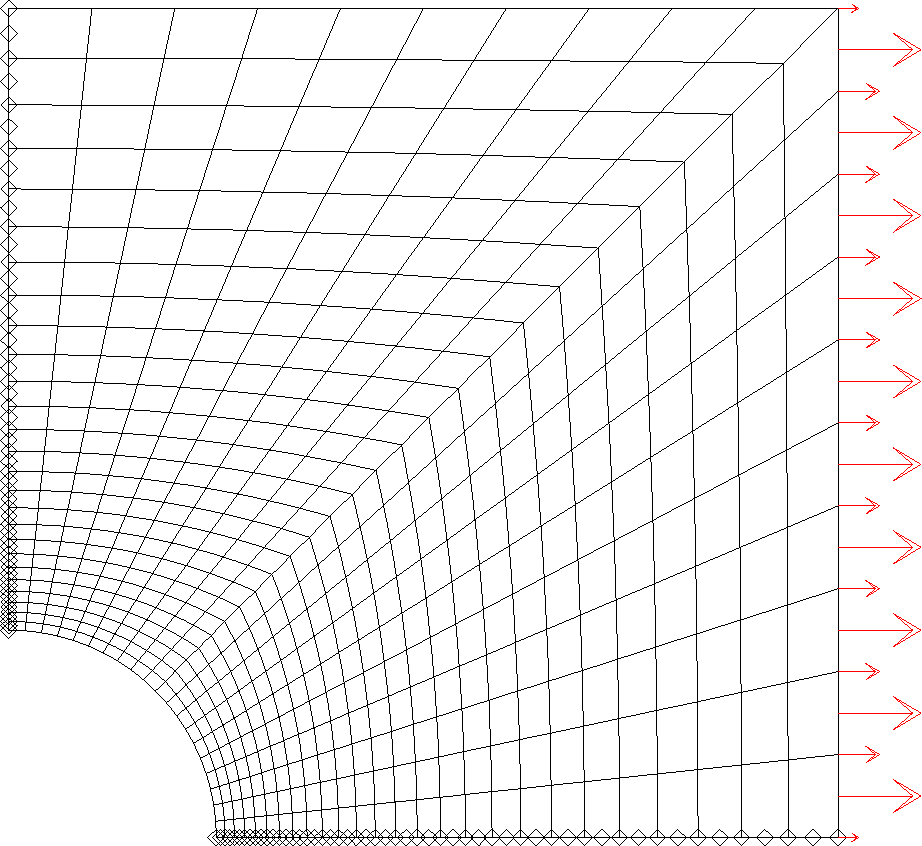
\includegraphics[height=0.25\textheight]{images/plaque.1} \:
      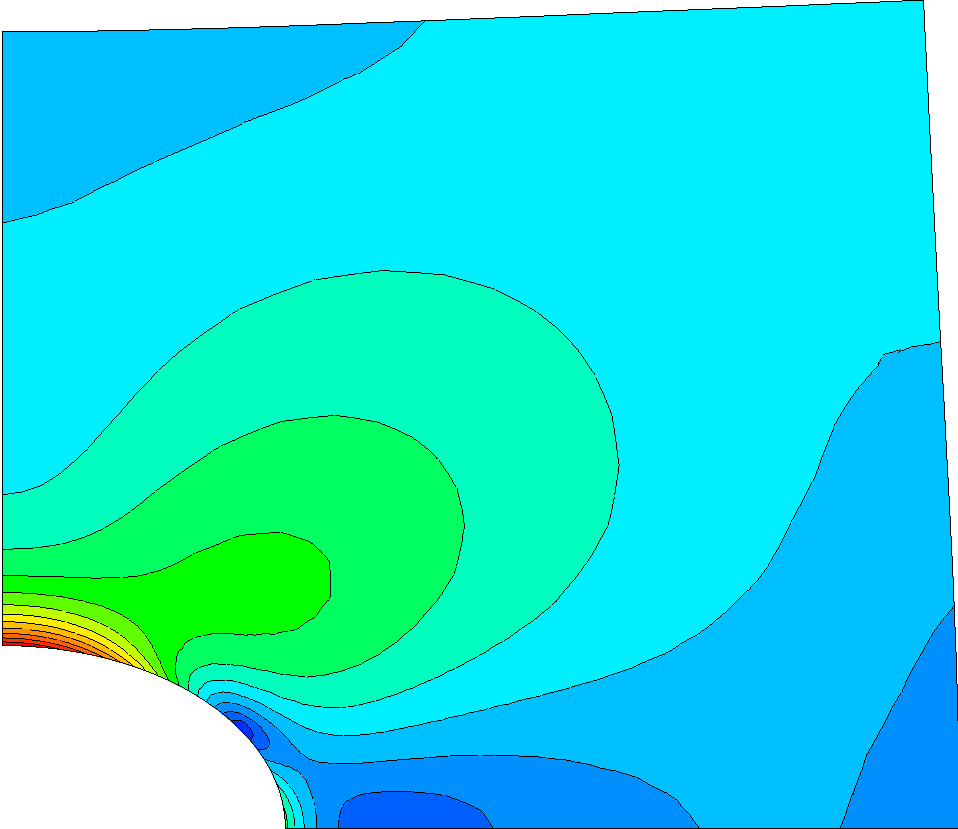
\includegraphics[height=0.25\textheight]{images/plaque.2} \:
      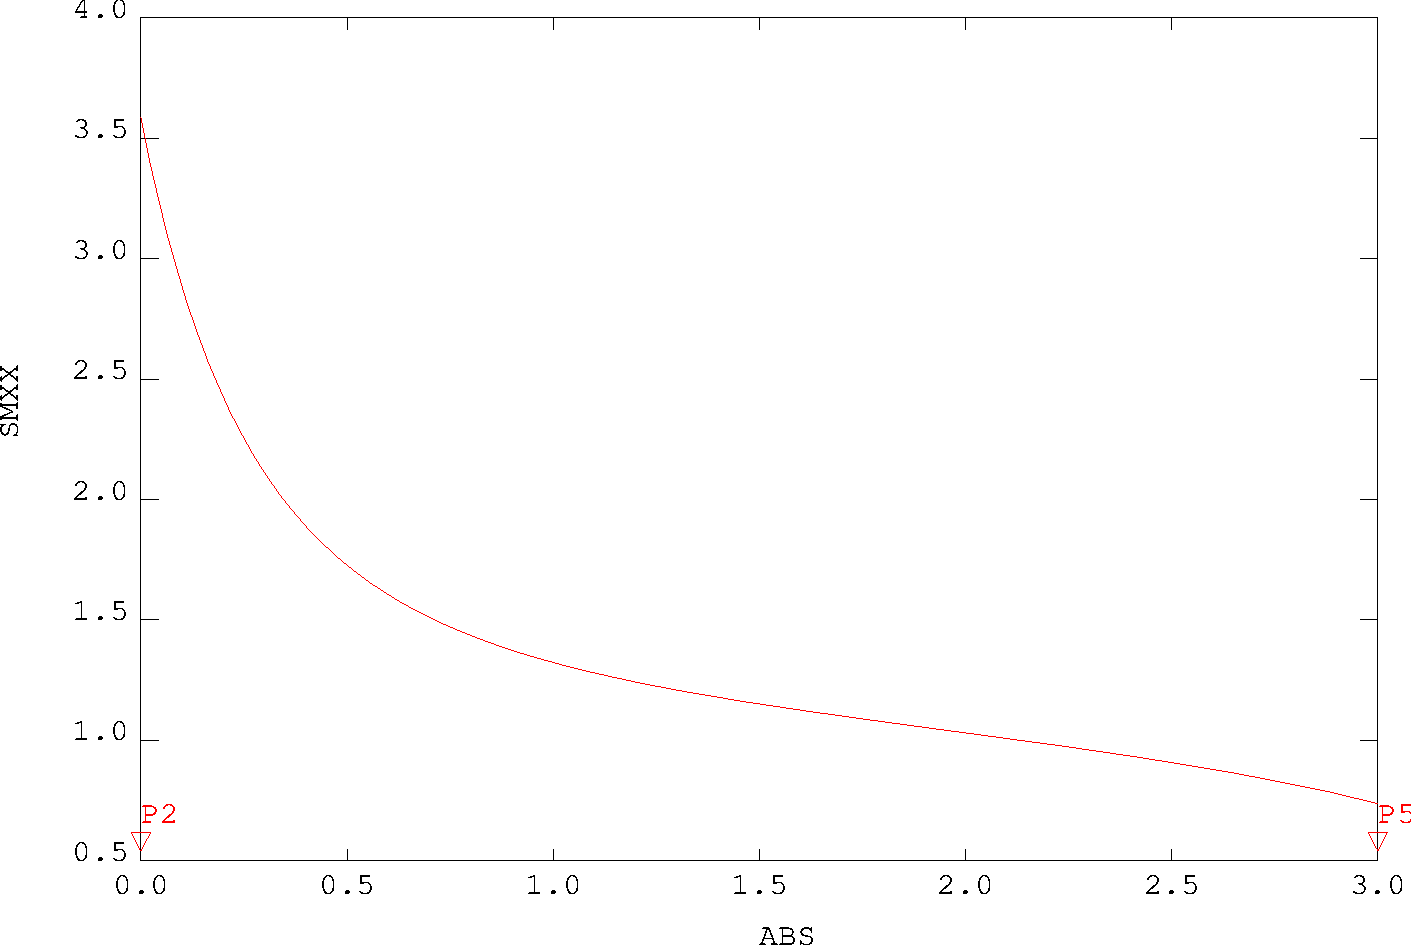
\includegraphics[height=0.25\textheight]{images/plaque.3}
    \end{center}\pause
    \item \fe{Basé sur un langage de commande : \g{Gibiane} (orienté objet)}
             {Based on a programming language: \g{Gibiane} (objet-oriented)}\\
  \end{itemize}
\end{frame}

\begin{frame}{\fe{Nombreux domaines d'application}{Wide range of applications}}
  \small{
  \begin{itemize}
    \item<1->\fe{\g{Mécanique des structures}}{\g{Structural mechanics}}\\
    \footnotesize{
    \fe{\red{Quasi-statique} (non linéarités matériau, géométrie, conditions limites)}
       {\red{Quasi-static} (non linear behavior, geometry, boundary conditions)}\\
    \onslide<1>{
      \begin{textblock*}{5cm}(2cm,0.3cm)
        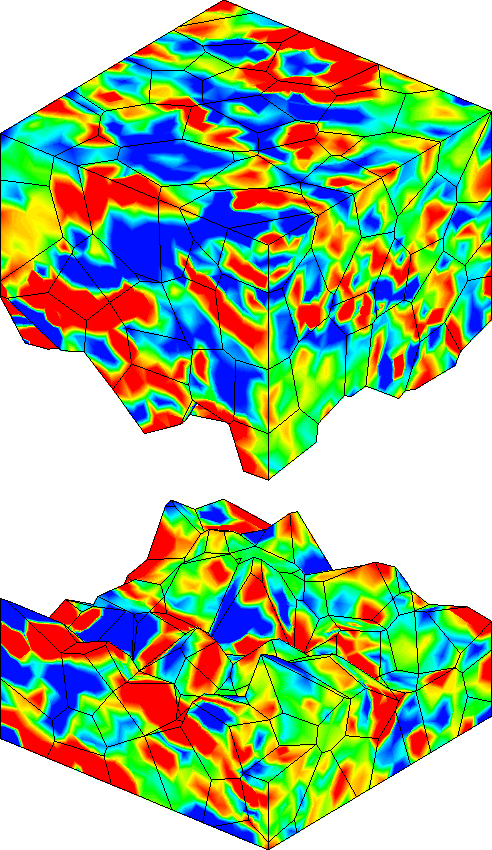
\includegraphics[height=0.4\textheight]{images/polycristal}
      \end{textblock*}
      \begin{textblock*}{5cm}(5cm,1.2cm)
        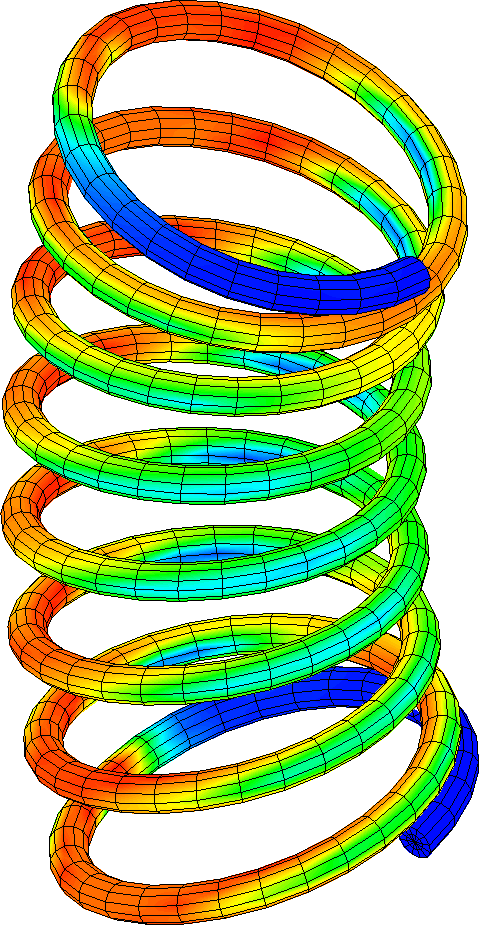
\includegraphics[height=0.4\textheight]{images/ressort}
      \end{textblock*}
      \begin{textblock*}{5cm}(8cm,2.1cm)
        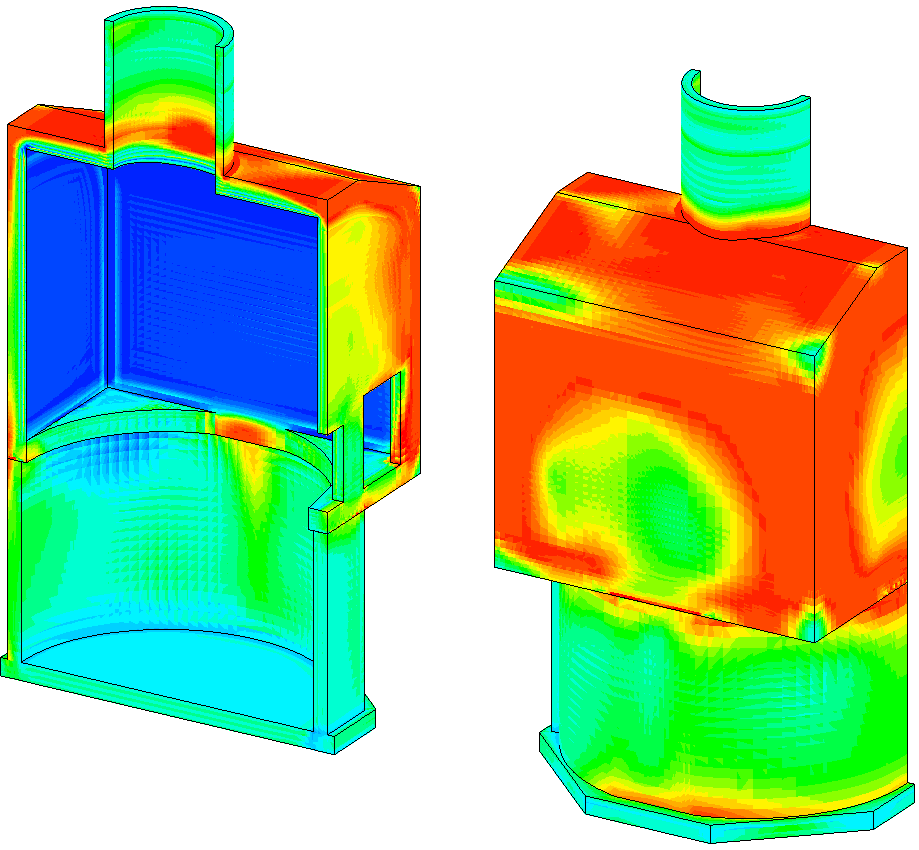
\includegraphics[height=0.4\textheight]{images/galatee}
      \end{textblock*}
      \begin{textblock*}{5cm}(9.4cm,5.6cm)
        \tiny{\emph{(S. Durand)}}
      \end{textblock*}}
    \onslide<2->\fe{\orange{Contact/frottement}, \green{Flambage}}
                    {\orange{Contact/friction}, \green{Buckling}}\\
    \onslide<2>{
      \begin{textblock*}{5cm}(1cm,0.3cm)
        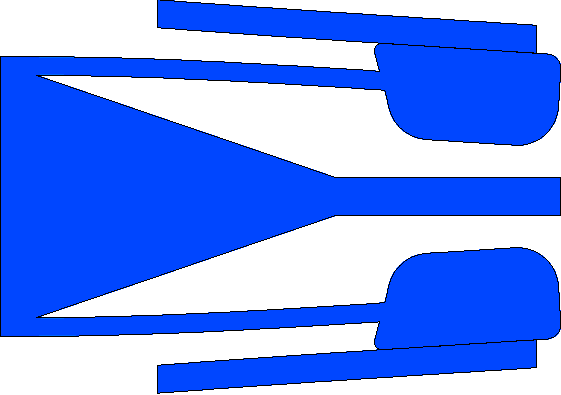
\includegraphics[height=0.25\textheight]{images/sac_a_dos.15}
      \end{textblock*}
      \begin{textblock*}{5cm}(4.8cm,0.3cm)
        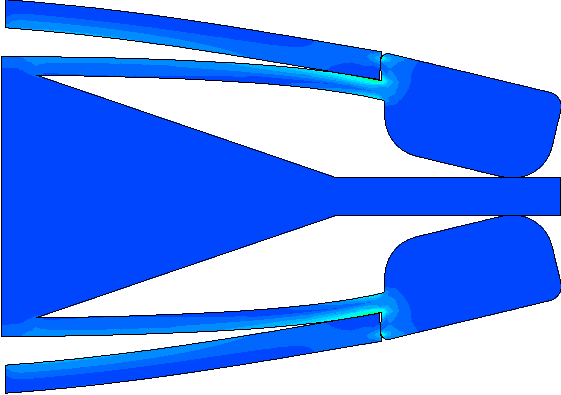
\includegraphics[height=0.25\textheight]{images/sac_a_dos.32}
      \end{textblock*}
    \begin{textblock*}{5cm}(8.5cm,0.3cm)
        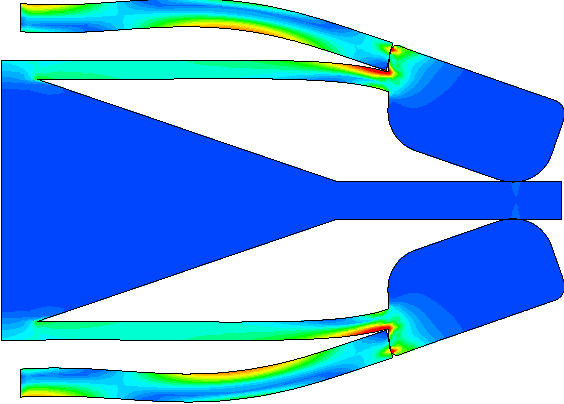
\includegraphics[height=0.25\textheight]{images/sac_a_dos.41}
      \end{textblock*}}
    \onslide<3->\fe{\blue{Dynamique} (temporelle, modale, interaction fluide structure)}
                    {\blue{Dynamic} (temporal, modal, fluid structure interaction)}\\
    \onslide<3>{
      \begin{textblock*}{5cm}(1cm,0.3cm)
        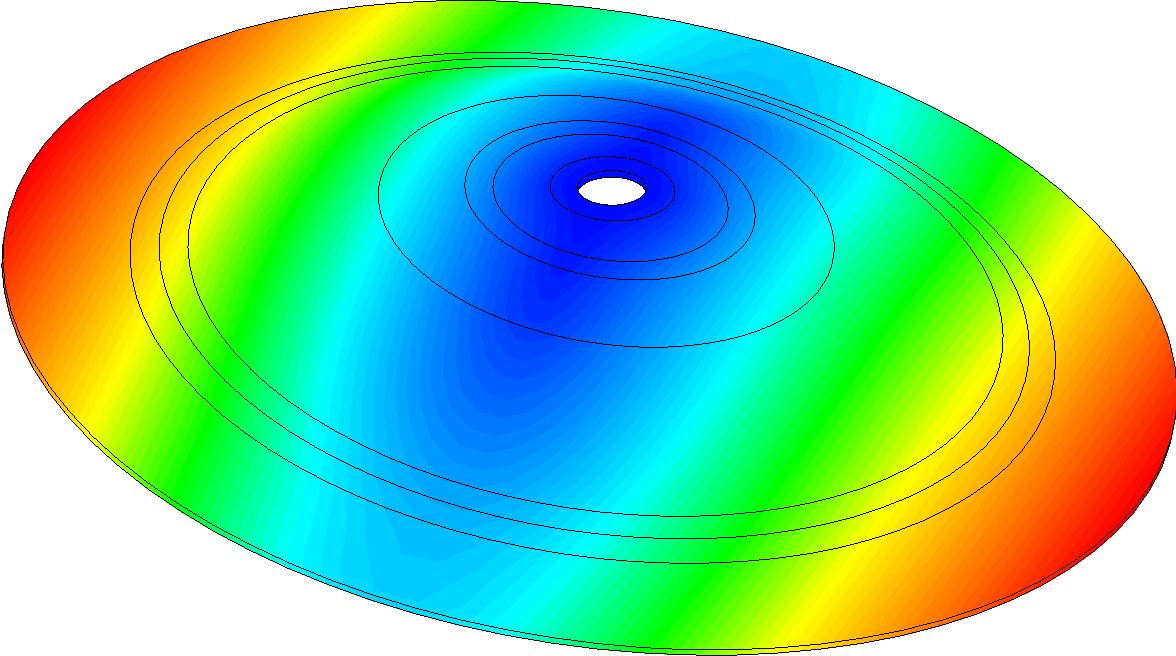
\includegraphics[height=0.2\textheight]{images/cymbale_mode_1}
      \end{textblock*}
      \begin{textblock*}{5cm}(4.8cm,0.3cm)
        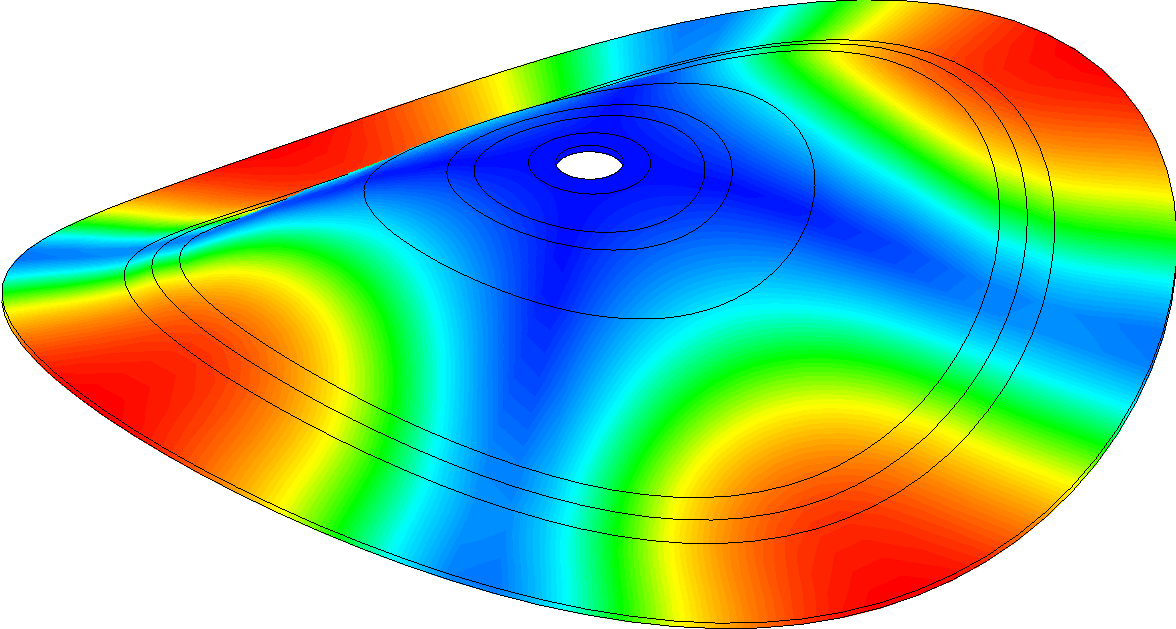
\includegraphics[height=0.2\textheight]{images/cymbale_mode_2}
      \end{textblock*}
      \begin{textblock*}{5cm}(8.5cm,0.3cm)
        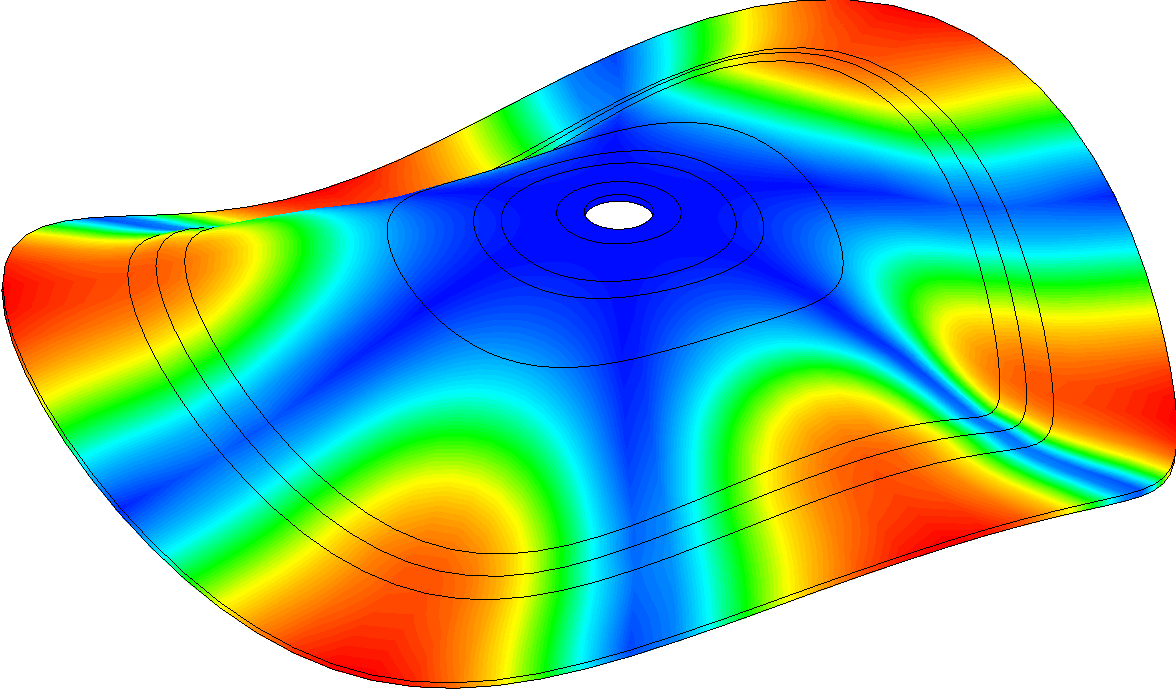
\includegraphics[height=0.2\textheight]{images/cymbale_mode_4}
      \end{textblock*}}
    \onslide<4->\fe{\violet{Rupture} (XFEM, propagation dynamique, zones cohésives)}
                   {\violet{Fracture} (XFEM, dynamic propagation, cohesive zones models)}\\
    \onslide<4>{
      \begin{textblock*}{12cm}(1.5cm,0.3cm)
        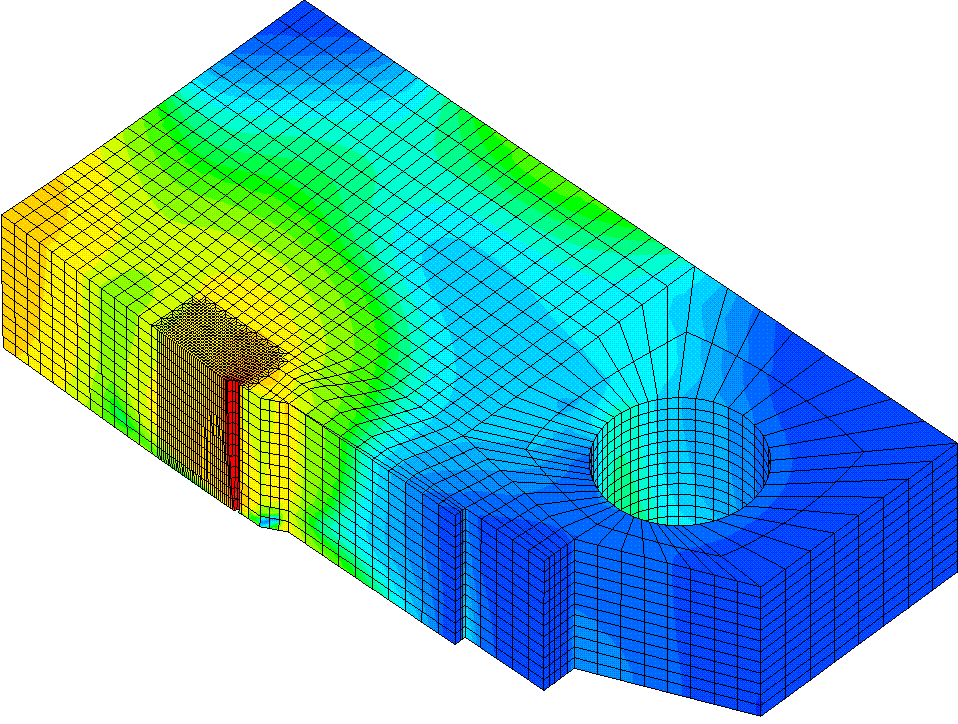
\includegraphics[height=0.25\textheight]{images/rousselier_03}
        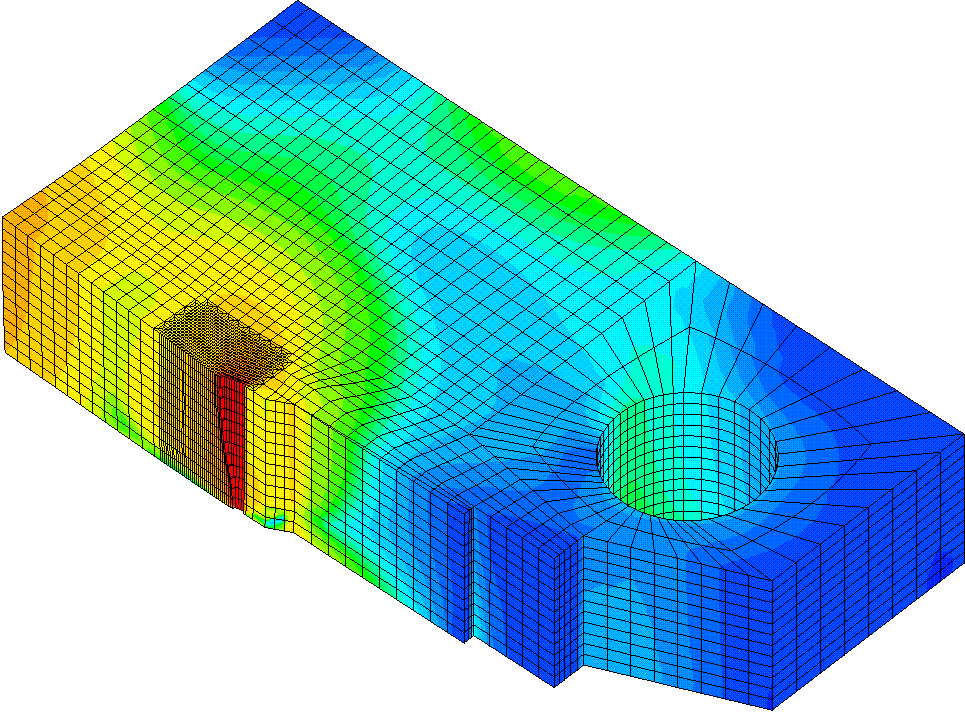
\includegraphics[height=0.25\textheight]{images/rousselier_04}
        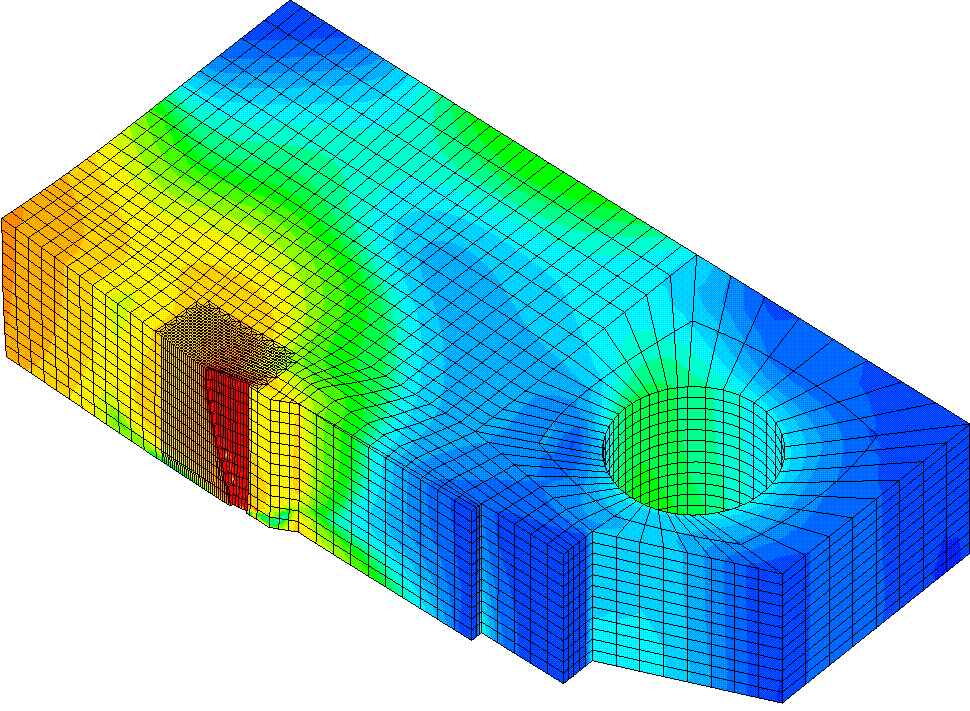
\includegraphics[height=0.25\textheight]{images/rousselier_05}\\
        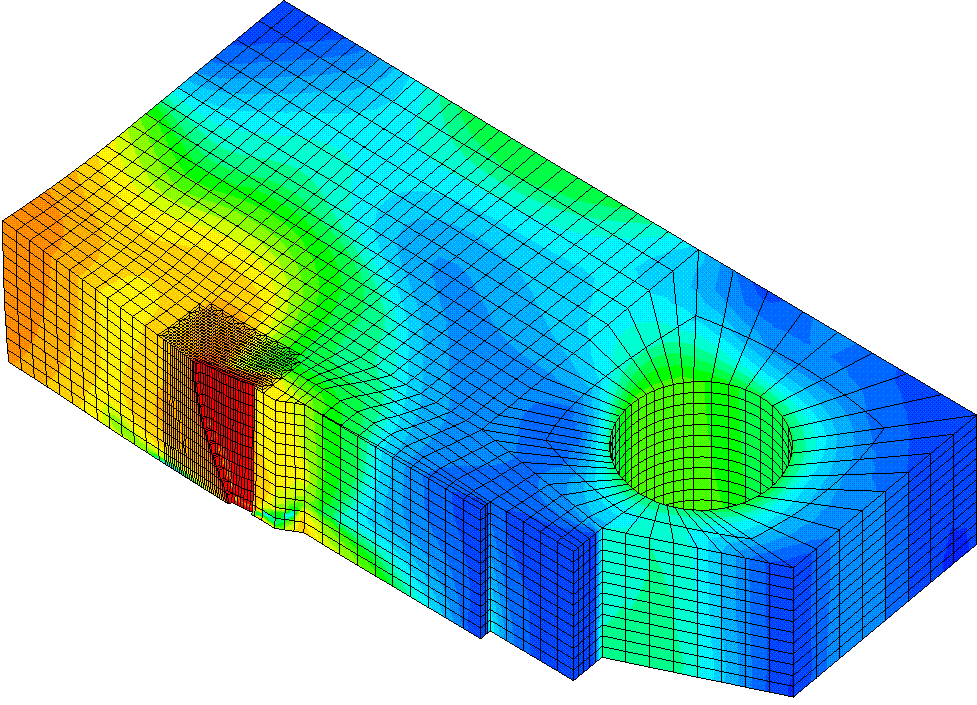
\includegraphics[height=0.25\textheight]{images/rousselier_06}
        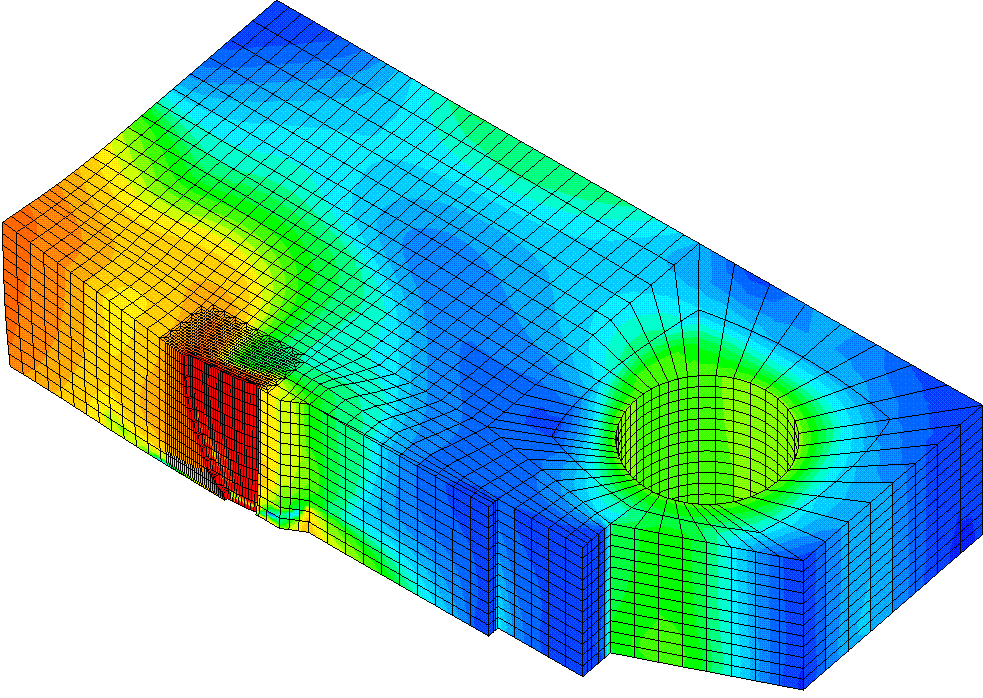
\includegraphics[height=0.25\textheight]{images/rousselier_07}
        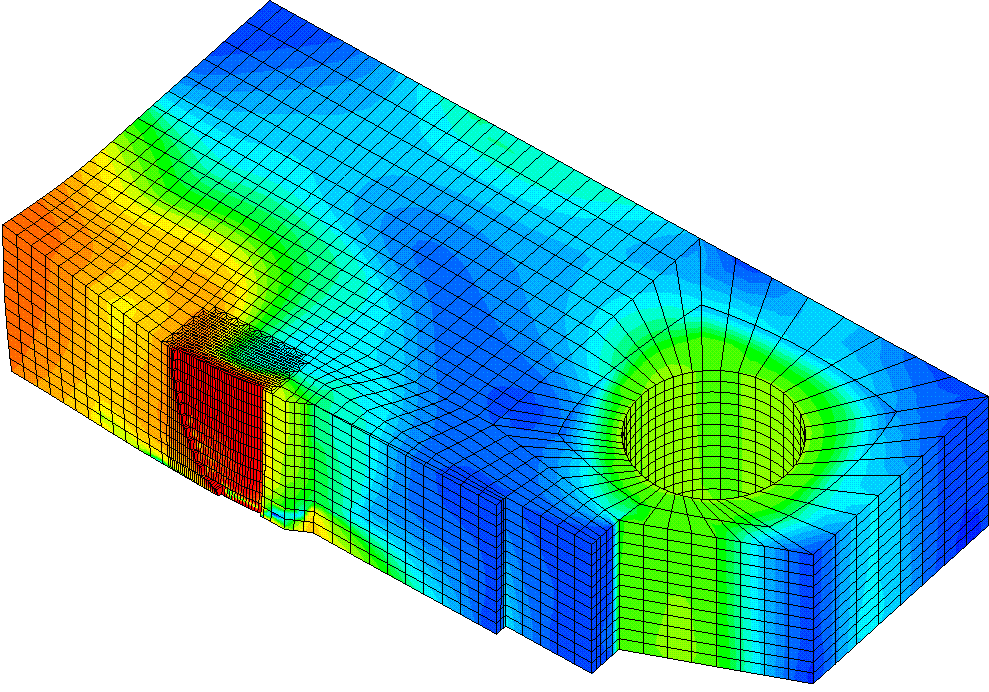
\includegraphics[height=0.25\textheight]{images/rousselier_08}
      \end{textblock*}
      \begin{textblock*}{5cm}(8cm,4.7cm)
        \tiny{\emph{(S. Kebiri)}}
      \end{textblock*}}
    \onslide<5>{
      \begin{textblock*}{12cm}(3.5cm,1.3cm)
        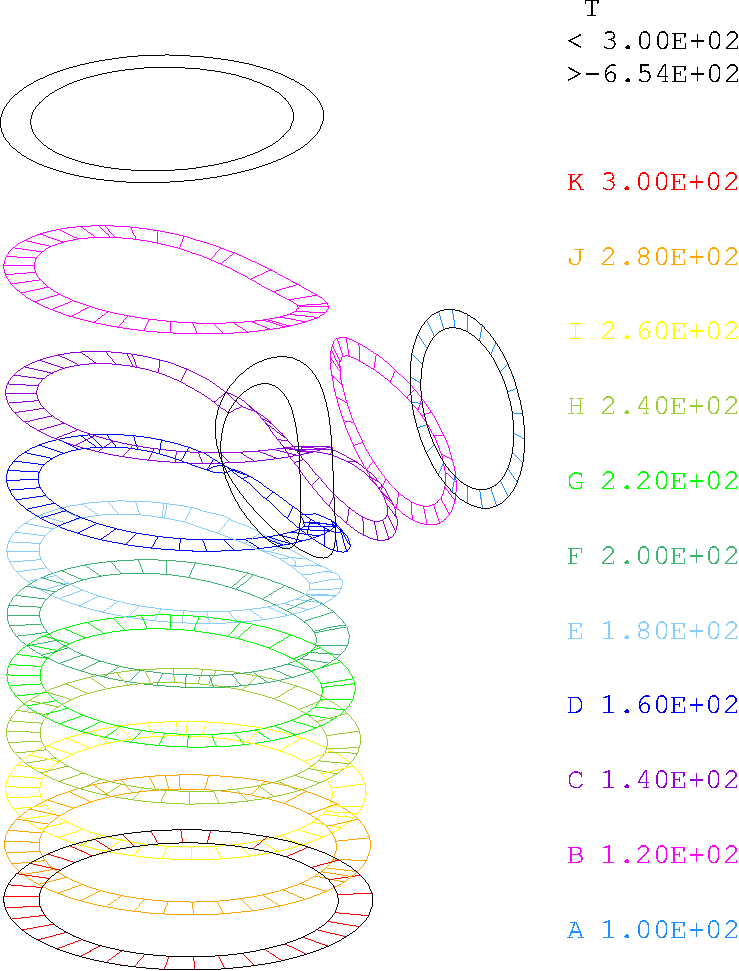
\includegraphics[height=0.4\textheight]{images/te_temperature}\hspace{1cm}
        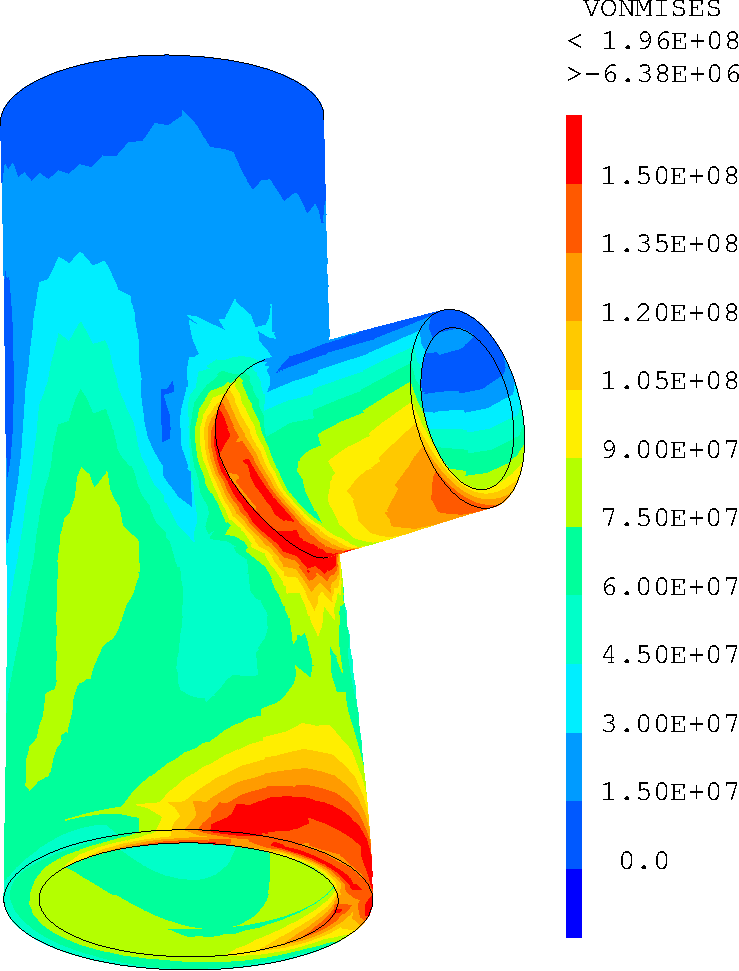
\includegraphics[height=0.4\textheight]{images/te_sigma}
      \end{textblock*}}
    \onslide<6>{
      \begin{textblock*}{12cm}(6.5cm,1.2cm)
        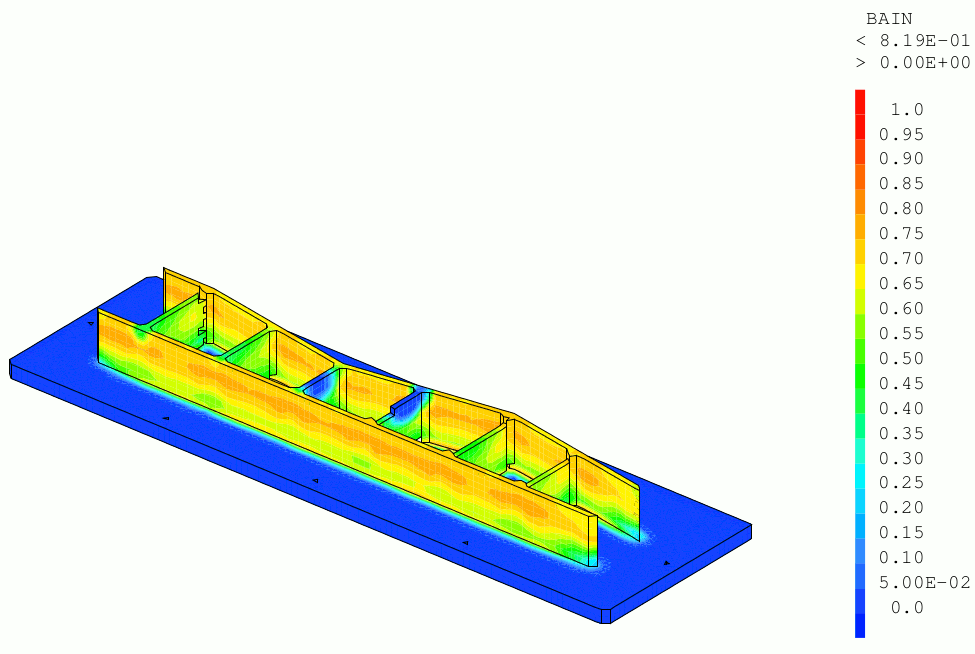
\includegraphics[height=0.4\textheight]{images/metallurgie}
      \end{textblock*}
      \begin{textblock*}{5cm}(8cm,4.7cm)
        \tiny{\emph{(C. Berthinier)}}
      \end{textblock*}}}
    \item<5->\fe{\g{Thermique}}{\g{Thermal analysis}}\\
    \footnotesize{
      \fe{Conduction, convection, rayonnement, changement de phase}
       {Conduction, convection, radiation, phase transition}}
    \item<6->\fe{\g{Mécanique des fluides}}{\g{Fluid mechanics}}
    \item<6->\fe{\g{Diffusion} multi espèces (loi de Fick)}{Multi species \g{diffusion} (Fick's law)}
    \item<6->\fe{Magnétostatique}{Magneto-statics}
    \item<6->\fe{Métallurgie}{Metallurgy}
    \item<6->\fe{Couplage thermo-hygro-mécanique}{Thermo-hygro-mechanics coupling}
  \end{itemize}}
\end{frame}

\begin{frame}{\fe{Présentation de PASAPAS}{The PASAPAS procedure}}
  \begin{itemize}
    \item \fe{Objectif}{Objective}\\
    \footnotesize
    \fe{Résolution de problèmes \emph{non linéaires évolutifs} de manière incrémentale\\
        en \red{thermique} et en \blue{mécanique}\\
        le temps peut être physique (ex~: thermique transitoire)\\
        ou non (ex~: plasticité avec chargement progressif)\\
        $\rightarrow$ on parle donc volontiers de \emph{variable d'évolution}\\}
       {Incremental solving of \emph{non linear progressive}\\
        \red{thermal} and \blue{mechanical} problems\\
        Time can be physical (e.g. thermal transients)\\
        or not (e.g. plasticity with progressive loading)\\
        $\rightarrow$ time or pseudo-time is called the \emph{evolution parameter}\\}
    ~
    \normalsize
    \item \fe{Types de non linéarités traitées}{Non linear phenomena considered}\\
    \fe{\red{Comportement} \footnotesize (plasticité, endommagement, matériaux variables, etc.) \normalsize\\
        \orange{Géométrie} \footnotesize (grands déplacements) \normalsize\\
        \green{Déformations} \footnotesize (grandes rotations) \normalsize\\
        \violet{Conditions limites} \footnotesize (rayonnement, frottement, pression suiveuse, etc.) \normalsize}
       {\red{Behavior} (plasticity, damage, variable material properties, etc.)\\
        \orange{Geometry} (large displacements)\\
        \green{Strains} (large rotations)\\
        \violet{Boundary conditions} (radiation, friction, following pressure, etc.)}
  \end{itemize}
\end{frame}

\begin{frame}{\fe{Utilisation de PASAPAS}{PASAPAS use}}
  \begin{itemize}
    \item \fe{\g{Créer une table} contenant toutes les données du problème}
             {\g{Create a table} containing all the data:}\\
    \lstinputlisting[language=gibiane, firstline=1, lastline=9]{dgibi/exemples.dgibi}
    \item \fe{\g{Appeler la procédure}}{\g{Procedure call:}}\\
    \lstinputlisting[language=gibiane, firstline=11, lastline=11]{dgibi/exemples.dgibi}
    \item \fe{\g{Post traitement} des résultats}{Results \g{post-processing}}
  \end{itemize}
\end{frame}

\begin{frame}{\fe{Aperçu des paramètres d'entrée}{Overview of input parameters}}
  \begin{itemize}
    \item \fe{Généralités}{General}\\
    \tiny
    \begin{tabular}{lll}
    \kwg{'MODELE'}           & MMODEL   & \fe{Équations à résoudre, formulation EF (\kwr{MODE})}
                                             {Equations to solve, FE formulation (\kwr{MODE})}\\
    \kwg{'CARACTERISTIQUES'} & MCHAML   & \fe{Paramètres matériau et/ou géométriques (\kwr{MATE})}
                                             {Material and/or geometrical parameters (\kwr{MATE})}\\
    \kwg{'CHARGEMENT'}       & CHARGEME & \fe{Évolution des CL et chargements au cours du calcul (\kwr{CHAR})}
                                             {BC and loading variation during calculation (\kwr{CHAR})}\\
    \end{tabular}
    \normalsize
    \item \fe{Thermique}{Thermal analysis}\\
    \tiny
    \begin{tabular}{lll}
    \kwg{'BLOCAGES\_THERMIQUES'} & RIGIDITE & \fe{Matrice de blocage des CL de type Dirichlet (\kwr{BLOQ})}
                                                 {Stiffness matrix for Dirichlet BC (\kwr{BLOQ})}\\
    \kwg{'CELSIUS'}              & LOGIQUE  & \fe{= VRAI si les températures sont en degrés Celsius}
                                                 {=VRAI (true) if temperature unit is Celsius}\\
    \kwg{'TEMPERATURES' . 0}     & CHPOINT  & \fe{Conditions initiales}
                                                 {Initial conditions}\\
    \end{tabular}
    \normalsize
    \item \fe{Mécanique}{Mechanics}\\
    \tiny
    \begin{tabular}{lll}
    \kwg{'BLOCAGES\_MECANIQUES'}           & RIGIDITE & \fe{Matrice de blocage des CL de type Dirichlet (\kwr{BLOQ})}
                                                           {Stiffness matrix for Dirichlet BC (\kwr{BLOQ})}\\
    \kwg{'GRANDS\_DEPLACEMENTS'}           & LOGIQUE  & \fe{Équilibre vérifié sur les configurations déformées}
                                                           {Equilibrium checked on the deformed mesh}\\
    \kwg{'DEPLACEMENTS' . 0}               & CHPOINT  & \fe{Conditions initiales}
                                                           {Initial conditions}\\
    \kwg{'CONTRAINTES' . 0}                & MCHAML   & Idem\\
    \kwg{'VARIABLES\_INTERNES' . 0}        & MCHAML   & Idem\\
    \kwg{'DEFORMATIONS\_INELASTIQUES' . 0} & MCHAML   & Idem\\
    \end{tabular}
    \normalsize
    \item \fe{Mécanique (dynamique)}{Mechanics (dynamics)}\\
    \tiny
    \begin{tabular}{lll}
    \kwg{'DYNAMIQUE'}          & LOGIQUE  & \fe{= VRAI si calcul dynamique}
                                               {= VRAI (true) for dynamics calculations}\\
    \kwg{'AMORTISSEMENT'}      & RIGIDITE & \fe{Matrice d’amortissement}
                                               {Damping matrix}\\
    \kwg{'VITESSES' . 0}       & MCHAML   & \fe{Conditions initiales}
                                               {Initial conditions}\\
    \kwg{'ACCELERATIONS' . 0 } & CHPOINT  & Idem\\
    \end{tabular}
    \normalsize
    \item \fe{Instants de calcul et sauvegarde}{Calculation and saving times}\\
    \tiny
    \begin{tabular}{lll}
    \kwg{'TEMPS\_CALCULES'} & LISTREEL & \fe{Liste des instants de calcul (\kwr{PROG})}
                                            {List of times for which results are computed (\kwr{PROG})}\\
    \kwg{'TEMPS\_SAUVES'}   & LISTREEL & \fe{Liste des instants pour lesquels les résultats sont conservés (\kwr{PROG})}
                                            {List of times for which results are saved (\kwr{PROG})}\\
    \end{tabular}
    \normalsize
  \end{itemize}
\end{frame}

\begin{frame}{\fe{Aperçu des paramètres de sortie}{Overview of ouput parameters}}
  \begin{itemize}
    \item \fe{Résultats}{Results}\\
    \tiny
    \begin{tabular}{lll}
    \kwg{'TEMPS'}                      & TABLE & \fe{Instants de calcul, identiques aux \kwg{'TEMPS\_SAUVES'}}
                                                    {Time values, identical to \kwg{'TEMPS\_SAUVES'}}\\
    & & \\
    \kwg{'TEMPERATURES'}               & TABLE & \fe{Champs solutions pour chaque \kwg{'TEMPS\_SAUVES'}}
                                                    {Fields (solution) calculated for each stored time \kwg{'TEMPS\_SAUVES'}}\\
    \kwg{'PROPORTION\_PHASE'}          & TABLE & Idem\\
    & & \\
    \kwg{'DEPLACEMENTS'}               & TABLE & Idem\\
    \kwg{'REACTIONS'}                  & TABLE & Idem\\
    \kwg{'CONTRAINTES'}                & TABLE & Idem\\
    \kwg{'DEFORMATIONS\_INELASTIQUES'} & TABLE & Idem\\
    \kwg{'VARIABLES\_INTERNES'}        & TABLE & Idem\\
    \kwg{'VITESSES'}                   & TABLE & Idem\\
    \kwg{'ACCELERATIONS'}              & TABLE & Idem\\
    \end{tabular}
    \normalsize
  \end{itemize}
\end{frame}

\begin{frame}{\fe{Exemples de post traitement}{Post processing examples}}
  \begin{itemize}
    \item \fe{Extraction des champs solution :}{Solution fields extraction:}\\
      \fe{avec l'indice dans la table}{from the table index}\\
      \lstinputlisting[language=gibiane, firstline=13, lastline=13]{dgibi/exemples.dgibi}
      \fe{ou bien avec l'instant de calcul}{or from the time value}\\
      \lstinputlisting[language=gibiane, firstline=14, lastline=14]{dgibi/exemples.dgibi}
    \item \fe{Tracé en mode graphique interactif :}{Graphical mode, interactive plot:}\\
    \lstinputlisting[language=gibiane, firstline=15, lastline=15]{dgibi/exemples.dgibi}
    \item \fe{Évolution temporelle d'un champ calculé :}{Evolution of calculated field with time:}\\
    \lstinputlisting[language=gibiane, firstline=16, lastline=16]{dgibi/exemples.dgibi}
  \end{itemize}
\end{frame}

%%%%%%%%%%%%%%%%%%%%%%%%%%%%%%%%%%%%%%%%%%%%%%%%%%%%%%%%%%%%%%%%%%%%%
\fe{\section{La procédure PASAPAS}}{\section{The PASAPAS procedure}}
\label{pasapas}
%%%%%%%%%%%%%%%%%%%%%%%%%%%%%%%%%%%%%%%%%%%%%%%%%%%%%%%%%%%%%%%%%%%%%

\begin{frame}{\fe{Algorithme de PASAPAS}{PASAPAS algorithm}}
  \begin{itemize}
    \item \fe{Initialisations}{Initializations}
    \item \fe{\green{Boucle sur les pas de temps}}{\green{Loop on time steps}}
    \begin{itemize}
      \item \fe{\red{Boucle de convergence thermo mécanique}}{\red{Loop for themo mechanical convergence}}
      \begin{itemize}
        \item \fe{\red{Solveur thermique}}{\red{Thermal solver}}
        \item \fe{\red{Solveur thermique}}{\red{Thermal solver}}
      \end{itemize}
      \item \fe{\red{Convergence thermo mécanique ?}}{\red{Thermo mechanical convergence?}}
    \end{itemize}
    \item \fe{\green{Enregistrement des résultats}}{\green{Save results}}
    \item \fe{Fin}{End}
  \end{itemize}
  \begin{center}
    \fe{+ Appels optionnels à des procédures utilisateur}{+ Optional user procedures calls}\\
    \kwv{PERSO1~~~PERSO2~~~REEV\_MEC~~~REEV\_THE}\\
    \kwv{CHARMECA~~~CHARTHER~~~PARATHER}\\
    \fe{ces procédures sont vides et à définir par l'utilisateur !}{procedures to be defined by the user!}
  \end{center}
\end{frame}

\begin{frame}{\fe{Algorithme de PASAPAS}{PASAPAS algorithm}}
  \tiny
  \begin{tikzpicture}[node distance=0.6cm,
    every node/.style={fill=white}, align=center]
  % Cellules (style, position, contenu)
  \fe{\node (start)  [bstep] {Initialisations,\\ \kwv{PERSO1}, \kwv{REEV\_MEC}, \kwv{REEV\_THE}};}
     {\node (start)  [bstep] {Initializations,\\ \kwv{PERSO1}, \kwv{REEV\_MEC}, \kwv{REEV\_THE}};}
  \fe{\node (start0) [note, right of=start, xshift=5.5cm] {Lecture des options, initialisations (matériaux, inconnues, chargements,\\
                                                           variables temporaires), instants de calcul, \dots\\
                                                           remplissage de \kw{tab1.}\kwg{'WTABLE'}};}
     {\node (start0) [note, right of=start, xshift=5cm] {Reading options, initializations (materials, unknowns, loading,\\
                                                          temporary variables), time steps, \dots\\
                                                          filling \kw{tab1.}\kwg{'WTABLE'}};}
  \fe{\node (init)  [gstep, below of=start, yshift=-0.1cm] {Initialisation du pas de temps};}
     {\node (init)  [gstep, below of=start, yshift=-0.1cm] {Time step initialization};}
  \fe{\node (resot) [rstep, below of=init]  {Résolution Thermique};}
     {\node (resot) [rstep, below of=init]  {Thermal solving};}
  \fe{\node (resot0) [note, right of=resot, xshift=5.5cm] {Appel à la procédure de calcul thermique \kwr{TRANSNON}\\
                                                           En grands déplacements, résolution sur dernière configuration déformée\\
                                                           Écriture des résultats dans \kw{tab1.}\kwg{'ESTIMATION'}};}
     {\node (resot0) [note, right of=resot, xshift=5.2cm] {Call of the procedure for thermal solver \kwr{TRANSNON}\\
                                                           In large displacements, solving on the last deformed configuration\\
                                                           Saving results in \kw{tab1.}\kwg{'ESTIMATION'}};}
  \node (rthe)  [rstep, below of=resot] {\kwv{REEV\_THE}};
  \fe{\node (rthe0) [note, right of=rthe, xshift=4.25cm] {Appel à la procédure \kwv{REEV\_THE} (si demandé)};}
     {\node (rthe0) [note, right of=rthe, xshift=4cm] {Call to the \kwv{REEV\_THE} procédure (if asked)};}
  \fe{\node (resom) [rstep, below of=rthe]  {Résolution Mécanique};}
     {\node (resom) [rstep, below of=rthe]  {Mechanical solving};}
  \fe{\node (resom0) [note, right of=resom, xshift=4.4cm] {Appel à la procédure de calcul mécanique \kwr{UNPAS}\\
                                                           Écriture des résultats dans \kw{tab1.}\kwg{'ESTIMATION'}};}
     {\node (resom0) [note, right of=resom, xshift=4.4cm] {Call of the procedure for mechanical solver \kwr{UNPAS}\\
                                                           Saving results in \kw{tab1.}\kwg{'ESTIMATION'}};}
  \node (rmec)  [rstep, below of=resom] {\kwv{REEV\_MEC}};
  \fe{\node (rmec0) [note, right of=rmec, xshift=4.25cm] {Appel à la procédure \kwv{REEV\_MEC} (si demandé)};}
     {\node (rmec0) [note, right of=rmec, xshift=4cm] {Call to the \kwv{REEV\_MEC} procedure (if asked)};}
  \node (contm) [rtest, below of=rmec, yshift=-0.3cm]  {Convergence ?};
  \fe{\node (contm0) [note, right of=contm, xshift=4.8cm] {Test de stationnarité, à activer avec :\\
                                                           \kw{tab1.}\kwg{'CONVERGENCE\_MEC\_THE'}\kw{ = VRAI ;}\\ \\
                                                           $\frac{\max \|T_i-T_{i-1}\|}{\max \|T_i\|} \le$ \kw{tab1.}\kwg{'CRITERE\_COHERENCE'} $(10^{-2})$};}
     {\node (contm0) [note, right of=contm, xshift=4.8cm] {Stationarity test, to be activated with:\\
                                                           \kw{tab1.}\kwg{'CONVERGENCE\_MEC\_THE'}\kw{ = VRAI ;}\\ \\
                                                           $\frac{\max \|T_i-T_{i-1}\|}{\max \|T_i\|} \le$ \kw{tab1.}\kwg{'CRITERE\_COHERENCE'} $(10^{-2})$};}
  \fe{\node (inip)  [gstep, below of=contm, yshift=-0.4cm] {Initialisation du pas de temps suivant};}
     {\node (inip)  [gstep, below of=contm, yshift=-0.4cm] {Initialize next time step};}
  \fe{\node (inip0) [note, right of=inip, xshift=5.5cm] {Enregistrement du nouvel état au début de pas dans : \kw{tab1.}\kwg{'WTABLE'}};}
     {\node (inip0) [note, right of=inip, xshift=5.4cm] {Saving the new state as the initial time step state in: \kw{tab1.}\kwg{'WTABLE'}};}
  \node (pers)  [gstep, below of=inip]  {\kwv{PERSO1}};
  \fe{\node (pers0) [note, right of=pers, xshift=4.25cm] {Appel à la procédure \kwv{PERSO1} (si demandé)};}
     {\node (pers0) [note, right of=pers, xshift=4cm] {Call to the \kwv{PERSO1} procedure (if asked)};}
  \fe{\node (sauv)  [gstep, below of=pers] {Sauvegarde des résultats};}
     {\node (sauv)  [gstep, below of=pers] {Saving results};}
  \fe{\node (sauv0) [note, right of=sauv, xshift=5.4cm] {\kwr{PAS\_RESU} : remplissage de \kwg{'CONTINUATION'} d'après \kwg{'ESTIMATION'}\\
                                                         \kwr{PAS\_SAUV} : écriture dans \kw{tab1} s'il s'agit d'un \kwg{'TEMPS\_SAUVE'}};}
     {\node (sauv0) [note, right of=sauv, xshift=5.2cm] {\kwr{PAS\_RESU}: filling \kwg{'CONTINUATION'} according to \kwg{'ESTIMATION'}\\
                                                         \kwr{PAS\_SAUV}: saving in \kw{tab1} if the time belong to \kwg{'TEMPS\_SAUVE'}};}
  \fe{\node (cont)  [gtest, below of=sauv, , yshift=-0.3cm]  {Fin des pas\\ de temps ?};}
     {\node (cont)  [gtest, below of=sauv, , yshift=-0.3cm]  {End of\\ time steps?};}
  \fe{\node (end)   [bstep, right of=cont, , xshift=2cm]  {Fin};}
     {\node (end)   [bstep, right of=cont, , xshift=2cm]  {End};}
% Connections entre les cellules
  \draw[->]             (start) -- (init);
  \draw[->, draw=Green] (init) -- (resot);
  \draw[->, draw=red]   (resot) -- (rthe);
  \draw[->, draw=red]   (rthe) -- (resom);
  \draw[->, draw=red]   (resom) -- (rmec);
  \draw[->, draw=red]   (rmec) -- (contm);
  \fe{\draw[->, draw=Green] (contm) -- node[xshift=0.4cm, yshift=0.1cm,]{oui} (inip);}
     {\draw[->, draw=Green] (contm) -- node[xshift=0.4cm, yshift=0.1cm,]{yes} (inip);}
  \fe{\draw[->, draw=red]   (contm.west) -- node[yshift=0.2cm]{non} ++(-0.55,0) -- ++(0,2.7) -- (resot.west);}
     {\draw[->, draw=red]   (contm.west) -- node[yshift=0.2cm]{no} ++(-0.55,0) -- ++(0,2.7) -- (resot.west);}
  \draw[->, draw=Green] (inip) -- (pers);
  \draw[->, draw=Green] (pers) -- (sauv);
  \draw[->, draw=Green] (sauv) -- (cont);
  \fe{\draw[->]             (cont) -- node[yshift=0.2cm,]{oui} (end);}
     {\draw[->]             (cont) -- node[yshift=0.2cm,]{yes} (end);}
  \fe{\draw[->, draw=Green] (cont.west) -- node[yshift=0.2cm]{non} ++(-0.6,0) -- ++(0,6.4) -- (init.west);}
     {\draw[->, draw=Green] (cont.west) -- node[yshift=0.2cm]{no} ++(-0.6,0) -- ++(0,6.4) -- (init.west);}
  \draw[dotted]         (start) -- (start0);
  \draw[dotted]         (resot) -- (resot0);
  \draw[dotted]         (rthe)  -- (rthe0);
  \draw[dotted]         (resom) -- (resom0);
  \draw[dotted]         (rmec)  -- (rmec0);
  \draw[dotted]         (contm) -- (contm0);
  \draw[dotted]         (inip)  -- (inip0);
  \draw[dotted]         (pers)  -- (pers0);
  \draw[dotted]         (sauv)  -- (sauv0);
  \end{tikzpicture}
\end{frame}

\begin{frame}{\fe{Accès aux données de PASAPAS}{Acces to PASAPAS data}}
  \begin{itemize}
    \item \kw{tab1.}\kwg{'ESTIMATION'}\\
    \footnotesize
    \fe{contient les résultats calculés par \kwr{TRANSNON} et \kwr{UNPAS}\\
        mais non convergées dans la \red{boucle de stationnarité thermo mécanique}}
       {contains all results calculated by \kwr{TRANSNON} and \kwr{UNPAS}\\
        but not converged for the \red{thermo mechanical stationarity loop}}
    \lstinputlisting[language=gibiane, firstline=18, lastline=22]{dgibi/exemples.dgibi}
    \normalsize
    \item \kw{tab1.}\kwg{'CONTINUATION'}\\
    \footnotesize
    \fe{contient les résultats calculés et convergés (pour la \red{boucle thermo mécanique})\\
        cet indice est mis à jour à la fin du pas de temps !\\
        utile pour une reprise de \kwr{PASAPAS}}
       {contains converged results for the \red{thermo mechanical loop}\\
        updated at the end of the time step!\\
        useful for \kwr{PASAPAS} restart}
    \lstinputlisting[language=gibiane, firstline=23, lastline=27]{dgibi/exemples.dgibi}
    \normalsize
  \end{itemize}
\end{frame}

\begin{frame}{\fe{Accès aux données de PASAPAS}{Acces to PASAPAS data}}
  \begin{itemize}
    \item \kw{tab1.}\kwg{'WTABLE'}\\
    \footnotesize
    \fe{Variables utiles à \kwr{PASAPAS} (options choisies, modèles, caractéristiques instanciées,\\
        chargements instanciés, résultats intermédiaires, \dots)}
       {All useful variables for \kwr{PASAPAS} (chosen options, models, INSTANCIEES properties,\\
        UPDATED loads, intermediate results, \dots)}\\~\\
    \fe{Quelques indices :}{Some indexes}
    \scriptsize
    \begin{tabular}{ll}
      \kwg{'WTABLE'} \kw{.} \kwg{'CHARGEMENT'}           & \fe{Chargement}{Loading}\\
      \kwg{'WTABLE'} \kw{.} \kwg{'THER\_COURANT'}        & \fe{Température à la dernière itération}{Value of temperature at last iteration}\\
                                                         & \fe{(au cours d'un pas)}{(during a time step)}\\
      \kwg{'WTABLE'} \kw{.} \kwg{'BLOCAGES\_MECANIQUES'} & \fe{Matrice de blocage mécanique}{Mechanical constraint matrix}\\
      \kwg{'WTABLE'} \kw{.} \kwg{'BLOCAGES\_THERMIQUES'} & \fe{Matrice de blocage thermique}{Thermal constraint matrix}\\
      \kwg{'WTABLE'} \kw{.} \kwg{'FOR'}                  & \fe{Configuration au début du pas}{Configuration at the time step beginning}\\
      \kwg{'WTABLE'} \kw{.} \kwg{'FOR0'}                 & \fe{Configuration initiale}{Initial configuration}\\
      \kwg{'WTABLE'} \kw{.} \kwg{'MODELE'}               & \fe{Modèles}{Modeles}\\
      \kwg{'WTABLE'} \kw{.} \kwg{'CARACTERISTIQUES'}     & \fe{Champ de caractéristiques matériau}{Material properties field}\\
      etc\dots&\\
    \end{tabular}
    \\~\\ \fe{Plus d'infos, voir les commentaires procédure \kwr{PAS\_DEFA}}
             {More information in the comments of the procedure \kwr{PAS\_DEFA}}
    \normalsize
  \end{itemize}
\end{frame}

%%%%%%%%%%%%%%%%%%%%%%%%%%%%%%%%%%%%%%%%%%%%%%%%%%%%%%%%%%%%%%%%
\fe{\section{Procédures utilisateur}}{\section{User procedures}}
\label{util_proc}
%%%%%%%%%%%%%%%%%%%%%%%%%%%%%%%%%%%%%%%%%%%%%%%%%%%%%%%%%%%%%%%%

\begin{frame}{\fe{Procédures utilisateur}{User procedures}}{\fe{Mode d'emploi}{Instructions for use}}
  \begin{itemize}
    \item[] \fe{Il existe 7 appels à des procédures utilisateurs\\ à différentes étapes de l'algorithme de \kwo{PASAPAS}}
               {There are 7 calls to user procedures\\ at different steps of \kwo{PASAPAS} algorithm}
    \begin{center}
      \kwv{PERSO1~~PERSO2~~REEV\_MEC~~REEV\_THE}\\
      \kwv{CHARMECA~~CHARTHER~~PARATHER}
    \end{center}
  \end{itemize}
  \begin{enumerate}
    \item \fe{\g{\blue{Choisir la procédure}}\\
              selon son emplacement dans \kwo{PASAPAS} et l'action désirée}
             {\g{\blue{Choose the procedure}}\\
              according to its location in \kwo{PASAPAS} and the action required}\\
    \scriptsize
    \fe{\ding{43}\emph{par exemple : puisque \kwv{PERSO1} est appelée après le calcul d'un pas de temps,\\
        ~~~elle peut servir à modifier le suivant (conditions aux limites, matériau \dots)}}
       {\ding{43}\emph{for instance: since \kwv{PERSO1} is called after computing a time step,\\
        ~~~it can be used to update the next one (boundary conditions, material \dots)}}
    \normalsize
    \item \fe{\g{\blue{Observer la syntaxe de la procédure}}\\
              dans le code de \kwv{PASAPAS} \dots~ou bien voir le tableau suivant}
             {\g{\blue{Analyze the procedure syntax}}\\
              in the \kwv{PASAPAS} code \dots~or see table on next slide}
  \end{enumerate}
\end{frame}

\begin{frame}{\fe{Procédures utilisateur}{User procedures}}{\fe{Mode d'emploi}{Instructions for use}}
  \begin{enumerate}\addtocounter{enumi}{2}
    \item \fe{\g{\blue{Définir la procédure}}
              \lstinputlisting[language=gibiane, firstline=29, lastline=31]{dgibi/exemples.dgibi}}
             {\g{\blue{Define the procedure}}
              \lstinputlisting[language=gibiane, firstline=32, lastline=34]{dgibi/exemples.dgibi}}
    \item \fe{\g{\blue{Brancher la procédure dans}} \kwo{PASAPAS}}
             {\g{\blue{Plug the procedure in}} \kwo{PASAPAS}}
          \lstinputlisting[language=gibiane, firstline=36, lastline=42]{dgibi/exemples.dgibi}
  \end{enumerate}
\end{frame}

\begin{frame}{\fe{Procédures utilisateur}{User procedures}}{\fe{Liste des procédures}{List of procedures}}
%  \begin{spacing}{1}
  \tiny
  \fe{\begin{tabular}{lllp{3cm}}
        \g{Procédure}             & \g{Indice dans la table PASAPAS}           & \g{Syntaxe}                                 & \g{Rôle possible} \\
        \hline\\
        \kwv{PERSO1}              & \kwg{'PROCEDURE\_PERSO1'~~}\kw{ = VRAI ;}  & \kwv{PERSO1 }\kw{tab1 ;}                    & Mise à jour du problème après calcul du pas mécanique\\
                                  &                                            &                                             & \\
        \kwv{REEV\_MEC}           & \kwg{'PROCEDURE\_REEV\_MEC'}\kw{ = VRAI ;} & \kwv{REEV\_MEC }\kw{tab1 n1 ;}              & Idem, mais dans la \red{boucle thermo mécanique}\\
                                  &                                            &                                             & \\
        \kwv{CHARMECA}            & \kwg{'PROCEDURE\_CHARMECA'}\kw{ = VRAI ;}  & \kw{tab2 = }\kwv{CHARMECA}\kw{ tab1 tps1 ;} & Ajout chargements mécaniques pendant \kwo{UNPAS}\\
                                  &                                            &                                             & \\
        \kwv{PERSO2}              & \kwg{'PROCEDURE\_PERSO2'~~}\kw{ = VRAI ;}  & \kwv{PERSO2 }\kw{tab1 ;}                    & Mise à jour du problème après calcul du pas thermique\\
                                  &                                            &                                             & \\
        \kwv{REEV\_THE}           & \kwg{'PROCEDURE\_REEV\_THE'}\kw{ = VRAI ;} & \kwv{REEV\_THE }\kw{tab1 n1 ;}              & Idem, mais dans la \red{boucle thermo mécanique}\\
                                  &                                            &                                             & \\
        \kwv{CHARTHER}            & \kwg{'PROCEDURE\_CHARTHER'}\kw{ = VRAI ;}  & \kw{tab2 = }\kwv{CHARTHER}\kw{ tab1 tps1 ;} & Ajout chargements thermiques pendant \kwo{TRANSNON}\\
                                  &                                            &                                             & \\
        \kwv{PARATHER}            & \kwg{'PROCEDURE\_PARATHER'}\kw{ = VRAI ;}  & \kwv{PARATHER}\kw{ tab1 tps1 ;}             & Mise à jour variables externes des caractéristiques thermiques\\
      \end{tabular}}
     {\begin{tabular}{lllp{3.2cm}}
        \g{Procedure}             & \g{Index in PASAPAS table}                 & \g{Syntax}                                  & \g{Possible function} \\
        \hline\\
        \kwv{PERSO1}              & \kwg{'PROCEDURE\_PERSO1'~~}\kw{ = VRAI ;}  & \kwv{PERSO1 }\kw{tab1 ;}                    & Updates the problem after the mechanical calculation step\\
                                  &                                            &                                             & \\
        \kwv{REEV\_MEC}           & \kwg{'PROCEDURE\_REEV\_MEC'}\kw{ = VRAI ;} & \kwv{REEV\_MEC }\kw{tab1 n1 ;}              & Ditto, but in the \red{thermo mechanical loop}\\
                                  &                                            &                                             & \\
        \kwv{CHARMECA}            & \kwg{'PROCEDURE\_CHARMECA'}\kw{ = VRAI ;}  & \kw{tab2 = }\kwv{CHARMECA}\kw{ tab1 tps1 ;} & Mechanical loads addition during \kwo{UNPAS} iterations\\
                                  &                                            &                                             & \\
        \kwv{PERSO2}              & \kwg{'PROCEDURE\_PERSO2'~~}\kw{ = VRAI ;}  & \kwv{PERSO2 }\kw{tab1 ;}                    & Updates the problem after the thermal calculation step\\
                                  &                                            &                                             & \\
        \kwv{REEV\_THE}           & \kwg{'PROCEDURE\_REEV\_THE'}\kw{ = VRAI ;} & \kwv{REEV\_THE }\kw{tab1 n1 ;}              & Ditto, but in the \red{thermo mechanical loop}\\
                                  &                                            &                                             & \\
        \kwv{CHARTHER}            & \kwg{'PROCEDURE\_CHARTHER'}\kw{ = VRAI ;}  & \kw{tab2 = }\kwv{CHARTHER}\kw{ tab1 tps1 ;} & Thermal loads addition during \kwo{TRANSNON} iterations\\
                                  &                                            &                                             & \\
        \kwv{PARATHER}            & \kwg{'PROCEDURE\_PARATHER'}\kw{ = VRAI ;}  & \kwv{PARATHER}\kw{ tab1 tps1 ;}             & Updating of the external variables of thermal parameters\\
      \end{tabular}}
  \fe{Avec :}{With:}
  \begin{tabular}{llll}
    \kw{tab1} & \fe{: la table de \kwo{PASAPAS}}{: the \kwo{PASAPAS} table}                                    & \kw{tps1} & \fe{: l'instant de calcul courant}{: the current calulated time}\\
    \kw{n1}   & \fe{: le numéro d'appel de la procédure (0 ou 1)}{: the call number of the procedure (0 or 1)} & \kw{tab2} & \fe{: la table de sortie (pour \kwv{CHARMECA} et \kwv{CHARTHER})}{: the output table (for \kwv{CHARMECA} et \kwv{CHARTHER})}
  \end{tabular}
  \normalsize
%  \end{spacing}
\end{frame}

\begin{frame}{\fe{Procédures utilisateur}{User procedures}}{\fe{Quelques remarques}{A few remarks}}
  \small
  \begin{itemize}
    \item \fe{Les instructions dans ces procédures sont libres !}{Instructions inside these procedures are free!}
    \item \fe{\kwo{CHARMECA} et \kwo{CHARTHER} doivent sortir une table, avec 2 indices possibles :}
             {\kwo{CHARMECA} and \kwo{CHARTHER} output is a table with 2 possible indexes:}
      \begin{tabular}{lp{7cm}}
        \kwg{'ADDI\_MATRICE'} & \fe{qui contient les matrices de RIGIDITE que l'on veut ajouter au 1er membre}
                                   {contains the stiffness matrices (RIGIDITE type object) to be added to the 1st member}\\
        \kwg{'ADDI\_SECOND'}  & \fe{qui contient les CHPOINT que l'on veut ajouter au 2nd membre (forces nodales, \dots)}
                                   {contains the CHPOINT to be added to the 2nd member (nodal forces, \dots)}
      \end{tabular}
    \item \fe{En grands déplacements (option \kwg{'GRANDS\_DEPLACEMENTS'})\\ \kwo{CHARMECA} est appelée sur la configuration déformée}
             {For large displacements (\kwg{'GRANDS\_DEPLACEMENTS'} option)\\ \kwo{CHARMECA} is called on the deformed shape}
  \end{itemize}
\end{frame}

\begin{frame}{\fe{Procédures utilisateur}{User procedures}}
             {\fe{Exemple : éprouvette entaillée en traction}
                 {Example: notched specimen under traction}}
  \footnotesize
  \begin{itemize}
    \begin{textblock*}{6cm}(8.5cm,0cm)
      \begin{tikzpicture}
        \node[anchor=south west,inner sep=0] (image) at (0,0)
        {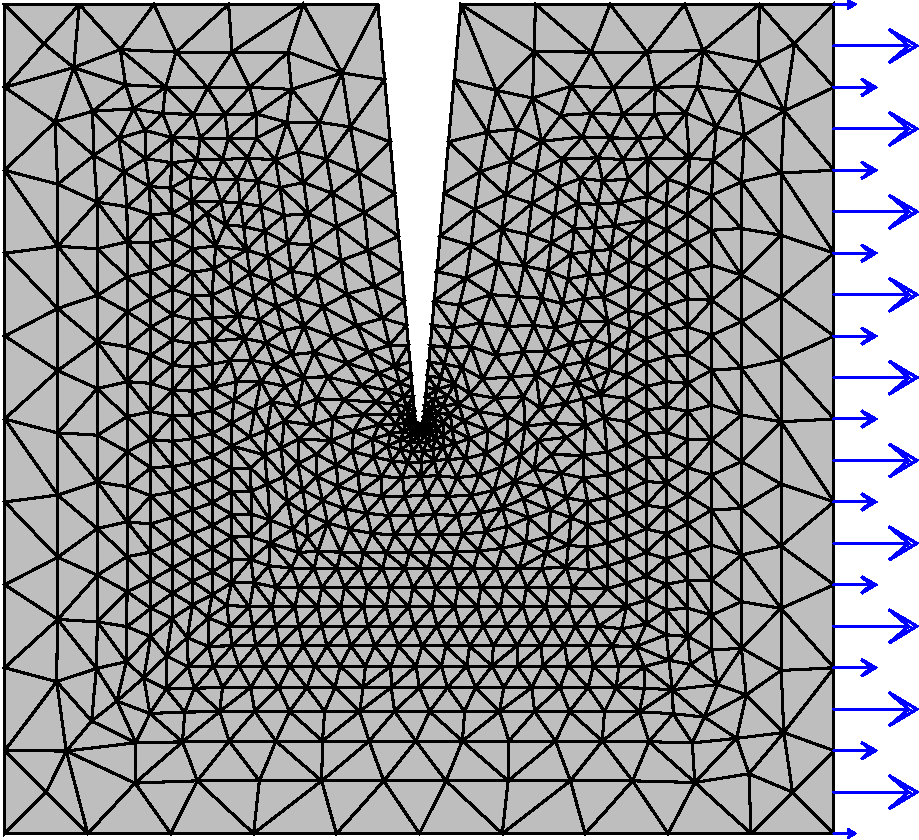
\includegraphics[width=3cm]{images/exemple/exemple_0.1}};
        \begin{scope}[x={(image.south east)},y={(image.north west)},color=black]
          \draw (0.37,1.04) node {\tiny \kw{p7}};
          \draw (0.55,1.04) node {\tiny \kw{p4}};
        \end{scope}
      \end{tikzpicture}
    \end{textblock*}
    \lstinputlisting[basicstyle=\ttfamily\tiny, language=gibiane, firstline=7, lastline=30]{dgibi/exemple_perso1.dgibi}
    \item[]
  \end{itemize}
\end{frame}

\begin{frame}{\fe{Procédures utilisateur}{User procedures}}
             {\fe{Exemple : éprouvette entaillée en traction}
                 {Example: notched specimen under traction}}
  \footnotesize
  \begin{itemize}
    \begin{textblock*}{6cm}(8.5cm,0.33cm)
      \begin{tikzpicture}
        \node[anchor=south west,inner sep=0] (image) at (0,0)
        {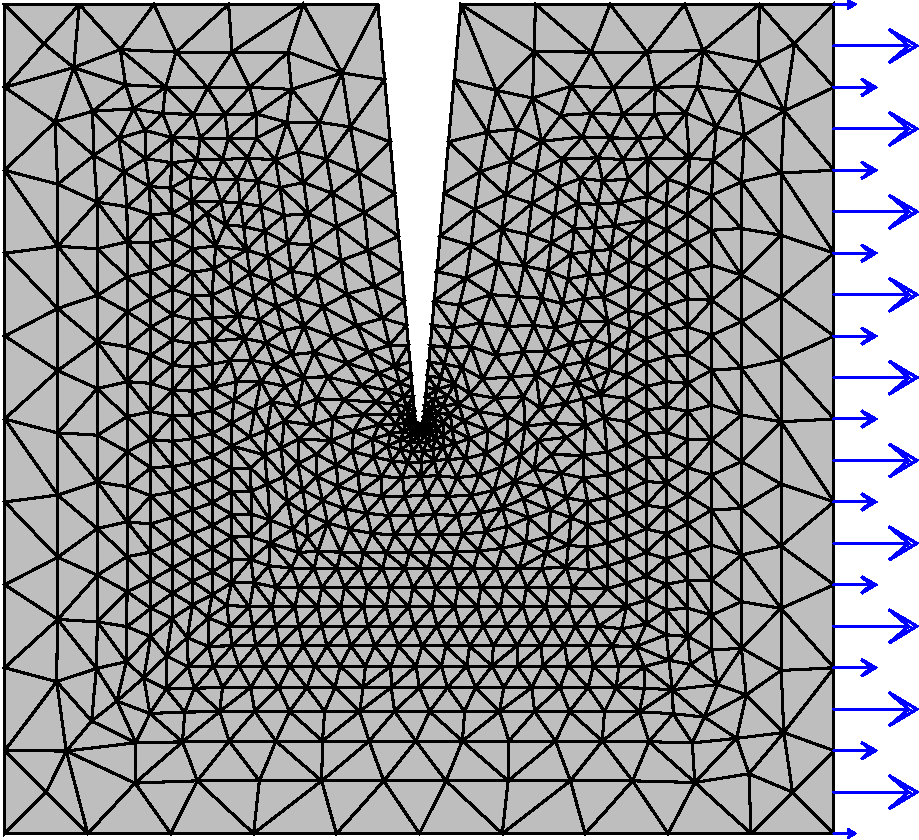
\includegraphics[width=3cm]{images/exemple/exemple_0.1}};
        \begin{scope}[x={(image.south east)},y={(image.north west)},color=black]
          \draw (0.37,1.04) node {\tiny \kw{p7}};
          \draw (0.55,1.04) node {\tiny \kw{p4}};
        \end{scope}
      \end{tikzpicture}
    \end{textblock*}
    \begin{textblock*}{6cm}(8.5cm,3.5cm)
      \animategraphics[controls,loop,poster=last,width=3.6cm]{10}{images/exemple/exemple_1.}{01}{21}
    \end{textblock*}
    \lstinputlisting[basicstyle=\ttfamily\tiny, language=gibiane, firstline=32, lastline=61]{dgibi/exemple_perso1.dgibi}
    \item[]
  \end{itemize}
\end{frame}

\begin{frame}{\fe{Procédures utilisateur}{User procedures}}
             {\fe{Exemple : éprouvette entaillée en traction \red{+ flexion pilotée par l'ouverture}}
                 {Example: notched specimen under traction \red{+ bending controled by opening}}}
  \footnotesize
  \begin{itemize}
    \begin{textblock*}{6cm}(8.5cm,0.33cm)
      \begin{tikzpicture}
        \node[anchor=south west,inner sep=0] (image) at (0,0)
        {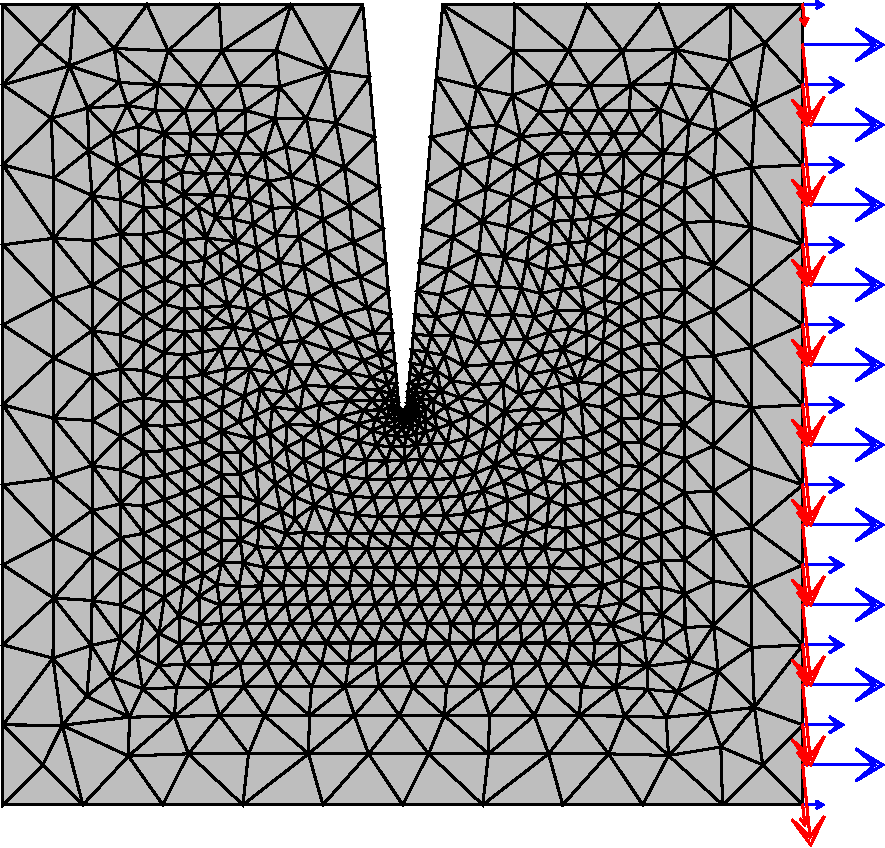
\includegraphics[width=3cm]{images/exemple/exemple_0.2}};
        \begin{scope}[x={(image.south east)},y={(image.north west)},color=black]
          \draw (0.37,1.04) node {\tiny \kw{p7}};
          \draw (0.55,1.04) node {\tiny \kw{p4}};
          \draw[<->, red] (0.41,1.) -- (0.5,1.);
          \draw (0.5,0.9) node[anchor=west, fill=white] {\tiny $\red{\Delta u}$};
        \end{scope}
      \end{tikzpicture}
    \end{textblock*}
    \begin{textblock*}{6cm}(8.5cm,3.5cm)
      \animategraphics[controls,loop,poster=last,width=3.6cm]{10}{images/exemple/exemple_2.}{01}{21}
    \end{textblock*}
    \lstinputlisting[basicstyle=\ttfamily\tiny, language=gibiane, firstline=68, lastline=97]{dgibi/exemple_perso1.dgibi}
    \item[]
  \end{itemize}
\end{frame}

%%%%%%%%%%%%%%%%%%%%%%%%%%%%%%%%%%%%%%%%%%%%%%%%%%%%%%%%%%%%%
\fe{\section{Solveur mécanique}}{\section{Mechanical solver}}
\label{mecanique}
%%%%%%%%%%%%%%%%%%%%%%%%%%%%%%%%%%%%%%%%%%%%%%%%%%%%%%%%%%%%%

\fe{\subsection{Équations}}{\subsection{Equations}}
\label{mecanique_equations}

\begin{frame}{\fe{Solveur mécanique}{Mechanical solver}}
             {\fe{Rappel des équations}{Reminder on equations}}
  \begin{itemize}
    \item<1->[] \fe{Équations locales du problème statique}
                   {Local equations of the static equilibrium}\\
    \scriptsize
    \fe{\begin{tabular}{lll}
          équilibre            & $\tx{div}(\tod{\sigma})+f_{\tx{imp}}=0$ & sur $\partial V$ \\
          efforts imposés      & $\tod{\sigma}.n=t_{\tx{imp}}$           & sur $\partial V_t$ \\
          déplacements imposés & $u=u_{\tx{imp}}$                        & sur $\partial V_u$ \\
        \end{tabular}}
       {\begin{tabular}{lll}
        equilibrium           & $\tx{div}(\tod{\sigma})+f_{\tx{imp}}=0$ & on $\partial V$ \\
        imposed forces        & $\tod{\sigma}.n=t_{\tx{imp}}$           & on $\partial V^t$ \\
        imposed displacements & $u=u_{\tx{imp}}$                        & on $\partial V^u$ \\
      \end{tabular}}
    \normalsize
    \onslide<2->{
    \begin{block}{\fe{Formulation faible + discrétisation EF}{Weak form + FE discretization}}
      \footnotesize
      \begin{equation*}
        \{F\}_{\tx{ext}}-\int_V[B]^T\{\sigma\}dV=\{0\}
      \end{equation*}
      \scriptsize
      \begin{equation*}
        \underbrace{\int_{\partial V_t}[N]^T\{t\}_{\tx{imp}}dS + \int_V[N]^T\{f\}_{\tx{imp}}dV}_{\{F\}_{\tx{imp}}} +
        \underbrace{\int_{\partial V_u}[N]^T\{\tod{\sigma}.n\}dS}_{\{F\}_{\tx{reac}}} -
        \underbrace{\int_V[B]^T\{\sigma\}dV}_{\{F\}_{\tx{int}}=[B]\{\sigma\}}=\{0\}
      \end{equation*}
    \end{block}}
    \item<3->[] \fe{Vecteurs de forces nodales équivalentes :}
                   {Equivalent nodal forces vector:}
    \scriptsize
    \begin{tabular}{lll}
      $\{F\}_{\tx{imp}}$  & \fe{forces volumiques $f_{\tx{imp}}$ et surfaciques $t_{\tx{imp}}$ imposées}
                               {imposed volume $f_{\tx{imp}}$ and surface $t_{\tx{imp}}$ forces}          & \kwr{PRES FSUR CNEQ}\\
      $\{F\}_{\tx{reac}}$ & \fe{réactions aux déplacements imposés $u_{\tx{imp}}$}
                               {reactions to imposed displacements $u_{\tx{imp}}$}                        & \kwr{REAC}\\
      $[B]\{\sigma\}$     & \fe{forces volumique intérieures}{internal volume forces}                     & \kwr{BSIG}
    \end{tabular}
  \end{itemize}
\end{frame}

\begin{frame}{\fe{Solveur mécanique}{Mechanical solver}}
             {\fe{Résidu}{Imbalance}}
  \begin{itemize}
    \item \fe{Résidu = mesure du déséquilibre}
             {Imbalance = measure of deviation of equilibrium}
    \begin{equation*}
      \{R\}=\{F\}_{\tx{imp}}+\{F\}_{\tx{reac}}-[B]\{\sigma\}
    \end{equation*}
    \item \fe{Équilibre atteint lorsque}{The balance is obtained when}
    \begin{equation*}
      \|R\| < \varepsilon F_{\tx{ref}}
    \end{equation*}
    \scriptsize
    \begin{tabular}{cl}
      $\|R\|$            & \fe{norme du résidu (par exemple la norme infinie)}
                              {norm of the imbalance vector (for instance infinity norm)}\\
      $\varepsilon$      & \fe{précision du calcul (fournie par utilisateur)}
                              {computational precision (given by user)}\\
      $\{F\}_{\tx{ref}}$ & \fe{effort de référence du problème considéré}
                              {reference force for the studied problem}
    \end{tabular}
  \end{itemize}
\end{frame}

\begin{frame}{\fe{Solveur mécanique}{Mechanical solver}}
             {\fe{Comportement non linéaire}{Non linear behavior}}
  \footnotesize
  \begin{itemize}
    \item<1-> \fe{Décomposition avec matrice de rigidité élastique linéaire}
                 {Decomposition with the linear elastic stiffness matrix}\\
    \begin{tabular}{lrrl}
      $\tod{\sigma}=\mathbb{E}:\tod{\varepsilon}_{\tx{lin}}+\tod{\sigma}_{\tx{nlin}}$ & \fe{avec}{with} & $\tod{\varepsilon}_{\tx{lin}}=$ & $\frac{1}{2}(\nabla u+\nabla^T u)$\\
       & & $\{\varepsilon\}_{\tx{lin}} =$ & $[B]\{U\}$
    \end{tabular}
    \item<2-> \fe{L'équilibre s'écrit alors}{Equilibrium can be re written}
    \begin{equation*}
      [B]\{\sigma\}=\{F\}_{\tx{imp}}+\{F\}_{\tx{reac}}
    \end{equation*}
    \begin{equation*}
      [B][E]\{\varepsilon\}_{\tx{lin}}=\{F\}_{\tx{imp}}+\{F\}_{\tx{reac}}-[B]\{\sigma\}_{\tx{nlin}}
    \end{equation*}
    \begin{equation*}
      \underbrace{\int_V[B]^T[E][B]dV}_{[K]}\{U\} =\{F\}_{\tx{imp}}+\{F\}_{\tx{reac}}-[B]\{\sigma\}_{\tx{nlin}}
    \end{equation*}
    \onslide<3->{
    \begin{equation*}
      [K]\{U\}=\{F\}_{\tx{imp}}+\{F\}_{\tx{reac}}-[B]\{\sigma\}_{\tx{nlin}}
    \end{equation*}\\~\\
    \scriptsize
    \begin{tabular}{llrl}
      $\{U\}$                      & \fe{déplacements nodaux}{nodal displacements}                                      & $u(x)=$                       & $[N(x)]\{U\}$\\
      $\{\varepsilon\}_{\tx{lin}}$ & \fe{déformations linéaires (petites déformations)}{linear strains (small strains)} & $\{\varepsilon\}_{\tx{lin}}=$ & $[B]\{U\}$\\
      $\{\sigma\}_{\tx{nlin}}$     & \fe{contraintes non linéaires}{non linear stresses}                                & & \\
      $[E]$                        & \fe{matrice de Hooke}{Hooke matrix}                                                & \kwr{ELAS} & \\
      $[K]$                        & \fe{matrice de rigidité élastique}{elastic stiffness matrix}                       & \kwr{RIGI} &
    \end{tabular}}
  \end{itemize}
\end{frame}

\begin{frame}{\fe{Solveur mécanique}{Mechanical solver}}
             {\fe{Prise en compte des déplacements imposés}{Introduction of the imposed displacements}}
  \begin{itemize}
    \item<1-> \fe{Matrice de blocage}{Boundary condition matrix}
    \scriptsize
    \begin{tabular}{rl}
      $u=$        & $u_{\tx{imp}}$ \quad \fe{sur}{on} $\partial V^u$\\
      $[A]\{U\}=$ & $\{u\}_{\tx{imp}}$
    \end{tabular}
    \normalsize
    \item<2-> \fe{Multiplicateurs de Lagrange}{Lagrange Multipliers}\\
    \scriptsize
    \fe{depuis un problème linéaire et sans contrainte :}{Ffom a linear and unconstraint problem:}
    $[K]\{U\}=\{F\}_{\tx{imp}}-[B]\{\sigma\}_{\tx{nlin}}$\\
    \fe{on ajoute les inconnues $\{\lambda\}$ :}{we add the unknowns $\{\lambda\}$:}
    \begin{equation*}
      [K]\{U\}+\underbrace{\red{[A]^T\{\lambda\}}}_{-\{F\}_{\tx{reac}}}=\{F\}_{\tx{imp}}-[B]\{\sigma\}_{\tx{nlin}} \quad \tx{\fe{avec}{with}} [A]\{U\}=\{u\}_{\tx{imp}}
    \end{equation*}
    \onslide<3->{
      \begin{block}{\fe{L'équilibre s'écrit alors :}{The equilibrium is now written:}}
        \begin{equation*}
          \underbrace{
            \begin{bmatrix}
              \green{K} & A^T\\
              A         & 0
            \end{bmatrix}}_{[\hat{K}]}
          \begin{Bmatrix}
            U\\
            \lambda
          \end{Bmatrix}
          =
          \begin{Bmatrix}
            \green{F_{\tx{imp}}}-\green{[B]\sigma_{\tx{nlin}}}\\
            u_{\tx{imp}}
          \end{Bmatrix}
        \end{equation*}
      \end{block}
    \scriptsize
    \fe{\begin{tabular}{lll}
          $[A]$              & matrice blocages/relations  & \kwr{BLOQ RELA}\\
          $\{u\}_{\tx{imp}}$ & déplacements nodaux imposés & \kwr{DEPI}\\
          $\{\lambda\}$      & multiplicateurs de Lagrange &
        \end{tabular}}
       {\begin{tabular}{lll}
        $[A]$         & constraints/relations matrix & \kwr{BLOQ RELA}\\
        $\{d\}$       & imposed nodal displacements  & \kwr{DEPI}\\
        $\{\lambda\}$ & Lagrange multipliers         &
      \end{tabular}}}\\
    \scriptsize
    \onslide<4->{
      $\green{[K],~\{F\}_{\tx{imp}},~[B]\{\sigma\}_{\tx{nlin}}}$
      \fe{dépendents de $\{U\}$ \tiny (comportement non lin., grands dépl., forces suiveuses \dots)}
         {depends on $\{U\}$ \tiny (non lin. behavior, large displacements, following forces \dots)}}
  \end{itemize}
\end{frame}


\begin{frame}{\fe{Solveur mécanique}{Mechanical solver}}
             {\fe{Décomposition incrémentale 1/2}{Incremental décomposition 1/2}}
  \begin{itemize}
    \item<1-> \fe{Calcul d'un pas de temps entre $t_0$ et $t_1$}
                 {Computation on a time step between $t_0$ and $t_1$}
    \scriptsize
    \begin{tabular}{lll}
      $\green{t_0~\{U\}_0~\{\lambda\}_0~\{\sigma\}_0}$ & \fe{\green{état connu}}{\green{known state}}                 & \fe{\green{début du pas de temps}}{\green{beginning of time step}}\\
      $  \red{t_1~\{U\}_1~\{\lambda\}_1~\{\sigma\}_1}$ & \fe{\red{état \tou{recherché}}}{\red{\tou{unknown} state}} & \fe{\red{fin du pas de temps}}{\red{end of time step}}\\
    \end{tabular}
    \item<2-> \fe{Décomposition incrémentale des déplacements nodaux}
                 {Incremental decomposition of nodal displacements}\\
    \scriptsize
    \begin{equation*}
      \red{\{U\}_1^i}=\green{\{U\}_0}+\red{\Delta \{U\}_1^i} \qquad \fe{\tx{et}}{\tx{and}} \qquad \red{\Delta \{U\}_1^{i+1}}=\red{\Delta \{U\}_1^i}+\violet{\delta \{U\}_1^{i+1}}
    \end{equation*}
    \fe{et donc}{and so}
    \begin{equation*}
      \red{\{U\}_1^{i+1}}=\red{\{U\}_1^i}+\violet{\delta \{U\}_1^{i+1}}
    \end{equation*}
    \scriptsize
    \begin{tabular}{ll}
      $\red{\{U\}_1^i}$               & \fe{estimation du déplacement $\red{\{U\}_1}$ à l’itération $i$}
                                           {estimation of displacement $\red{\{U\}_1}$ at iteration $i$}\\
      $\red{\Delta \{U\}_1^i}$        & \fe{estimation de l'incrément de déplacement à l’itération $i$}
                                           {estimation of displacement increment at iteration $i$}\\
      $\violet{\delta \{U\}_1^{i+1}}$ & \fe{correction de l’incrément de déplacement à l’itération $i$}
                                           {correction of displacement increment at iteration $i$}
    \end{tabular}
    \item<3-> \fe{Décomposition incrémentale des conditions sur les déplacements}
                 {Incremental decomposition of boundary conditions}
    \scriptsize
    \begin{equation*}
      [A]\red{\{U\}_1^{i+1}}=\{u\}_{\tx{imp},1}
    \end{equation*}
    \begin{equation*}
      [A]\violet{\delta\{U\}_1^{i+1}}=\{u\}_{\tx{imp},1}-[A]\red{\{U\}_1^i}
    \end{equation*}
  \end{itemize}
\end{frame}

\begin{frame}{\fe{Solveur mécanique}{Mechanical solver}}
             {\fe{Décomposition incrémentale 2/2}{Incremental décomposition 2/2}}
  \begin{itemize}
    \item<1-> \fe{Décomposition incrémentale de l’équilibre}
                 {Incremental decomposition of equilibrium}
    \scriptsize
    \begin{equation*}
      [K]\red{\{U\}_1^{i+1}}+[A]^T\red{\{\lambda\}_1^{i+1}} = \{F\}_{\tx{imp},1} - [B]\red{\{\sigma\}_{\tx{nlin},1}^i}
    \end{equation*}
    \begin{equation*}
      [K]\violet{\delta\{U\}_1^{i+1}} = \{F\}_{\tx{imp},1} - [A]^T\red{\{\lambda\}_1^{i+1}} - \underbrace{([K]\red{\{U\}_1^i} + [B]\red{\{\sigma\}_{\tx{nlin},1}^i})}_{[B]\red{\{\sigma\}_1^i}}
    \end{equation*}
    \begin{equation*}
      [K]\violet{\delta\{U\}_1^{i+1}} = \underbrace{\{F\}_{\tx{imp},1} - [A]^T\red{\{\lambda\}_1^{i+1}} - [B]\red{\{\sigma\}_1^i}}_{\red{\{R\}_1^i}}
    \end{equation*}
    \normalsize
    \onslide<2->{
      \begin{block}{\fe{L’équilibre s’écrit finalement}{Equilibrium is finally written}}
        \begin{equation*}
          \underbrace{
            \begin{bmatrix}
              K & A^T\\
              A & 0
            \end{bmatrix}}_{[\hat{K}]}
          \begin{Bmatrix}
            \violet{\delta U_1^{i+1}}\\
            \red{\lambda_1^{i+1}}
          \end{Bmatrix}
          =
          \begin{Bmatrix}
            F_{\tx{imp}}-[B]\red{\sigma_1^i}\\
            u_{\tx{imp},1}-[A]\red{U_1^i}
          \end{Bmatrix}
        \end{equation*}
      \end{block}}
  \end{itemize}
\end{frame}




\fe{\subsection{La procédure UNPAS}}{\subsection{The UNPAS procedure}}
\label{unpas}

\begin{frame}{\fe{Algoritme de minimisation du résidu}{Imbalance minimization algorithm}}
  \begin{itemize}
    \item<1-> \fe{Initialisations}{Initializations}
    \scriptsize
    \begin{tabular}{ll}
      &\\
      $\left[\red{\{U\}_1^{i=0}~\{\lambda\}_1^{i=0}~\{\sigma\}_1^{i=0}}\right] = \left[\green{\{U\}_0~\{\lambda\}_0~\{\sigma\}_0^{\white{0}}}\right]$ & \fe{initialisation de la solution}{solution initialization} \vspace{1mm}\\
      $\red{\{F\}_{\tx{reac},1}^{i=0}} = -[A]^T\red{\{\lambda\}_1^{i=0}}$                                           & \fe{initialisation des réactions \kwr{REAC}}{reactions initialization \kwr{REAC}} \vspace{1mm}\\
      $F_{\tx{ref}} = \|\{F\}_{\tx{imp},1}+\red{\{F\}_{\tx{reac},1}^{i=0}}\|$                                       & \fe{norme de convergence \kwr{MAXI}\kwg{ 'ABS'}}{convergence norm \kwr{MAXI}\kwg{ 'ABS'}} \vspace{1mm}\\
      $\{R\}_1^{i=0} = \{F\}_{\tx{imp},1}+\red{\{F\}_{\tx{reac},1}^{i=0}}-[B]\red{\{\sigma\}_1^{i=0}}$              & \fe{premier résidu \kwr{BSIG}}{first imbalance (residual) \kwr{BSIG}}\\
      &
    \end{tabular}
    \normalsize
    \item<2-> \fe{Tant que : $\|\{R\}_1^i\| \geq \varepsilon F_{\tx{ref}}$}{While: $\|\{R\}_1^i\| \geq \varepsilon F_{\tx{ref}}$}
    \begin{textblock*}{2.5cm}(9.5cm,-3.9cm)
      
\includegraphics[width=3cm]{images/obi_wan}
    \end{textblock*}
    \scriptsize
    \begin{tabular}{ll}
      &\\
      $\left[\violet{\delta\{U\}_1^{i+1}}~\red{\{\lambda\}_1^{i+1}}\right] = [\hat{K}]^{-1}\{R\}_1^i$ & \fe{résolution \kwr{RESO}}{resolution \kwr{RESO}} \vspace{1mm}\\
      $\red{\{U\}_1^{i+1}} = \red{\{U\}_1^i} + \violet{\delta\{U\}_1^{i+1}}$               & \fe{estim. déplacements}{estim. displacements} \vspace{1mm}\\
      $\red{\{\varepsilon\}_1^{i+1}} = \mathcal{D}(\red{\{U\}_1^{i+1}})$                   & \fe{estim. déformations \kwr{EPSI}}{estim. strains \kwr{EPSI}} \vspace{1mm}\\
      $\red{\{\sigma\}_1^{i+1}} = \mathcal{C}(\Delta\{\varepsilon\}_1^{i+1})$              & \fe{estim. contraintes \kwr{COMP}}{estim. stresses \kwr{COMP}} \vspace{1mm}\\
      $\red{\{F\}_{\tx{reac},1}^{i+1}} = -[A]^T\red{\{\lambda\}_1^{i+1}}$                  & \fe{estim. réactions \kwr{REAC}}{estim. reactions \kwr{REAC}} \vspace{1mm}\\
      $\{R\}_1^{i+1} = \{F\}_{\tx{imp},1}+\red{\{F\}_{\tx{reac},1}^{i+1}}-[B]\red{\{\sigma\}_1^{i+1}}$ & \fe{nouveau résidu \kwr{BSIG}}{new imbalance \kwr{BSIG}}
    \end{tabular}
    \normalsize
    \item<2->[] \fe{Fin}{End}
  \end{itemize}
\end{frame}

\begin{frame}{\fe{Algorithme de UNPAS}{UNPAS algorithm}}
  \tiny
  \begin{tikzpicture}[node distance=0.55cm,
    every node/.style={fill=white}, align=center]
  % Cellules (style, position, contenu)
  \fe{\node (ini)   [bstep] {Initialisations, \kwv{CHARMECA}};}
     {\node (ini)   [bstep] {Initializations, \kwv{CHARMECA}};}
  \fe{\node (ini0)  [note, right of=ini, xshift=1.5cm, anchor=west] {Instanciations matériaux, calcul matrice de rigidité $[K]$, forces imposées $\{F\}_{\tx{imp}}$};}
     {\node (ini0)  [note, right of=ini, xshift=1.5cm, anchor=west] {Material updating, stiffness matrix $[K]$ calculation, imposed forces $\{F\}_{\tx{imp}}$};}

  \fe{\node (1r)    [bstep, below of=ini] {1er résidu};}
     {\node (1r)    [bstep, below of=ini] {1st imbalance};}
  \fe{\node (1r0)   [note, right of=1r, xshift=1.5cm, anchor=west] {Déséquilibre entre les forces internes et externes\\
                                                                  $\{R\}_1^{i=0}=\{F\}_{\tx{imp},1}+\green{\{F\}_{\tx{reac},0}}-[B]\green{\{\sigma\}_0}$ \kwr{BSIG}};}
     {\node (1r0)   [note, right of=1r, xshift=1.5cm, anchor=west] {Imbalance between the internal and external forces\\
                                                                  $\{R\}_1^{i=0}=\{F\}_{\tx{imp},1}+\green{\{F\}_{\tx{reac},0}}-[B]\green{\{\sigma\}_0}$ \kwr{BSIG}};}

  \fe{\node (1res)  [rstep, below of=1r, yshift=-0.1cm] {1er \kwr{RESO}\\ norme de convergence};}
     {\node (1res)  [rstep, below of=1r, yshift=-0.1cm] {1st \kwr{RESO}\\ convergence norm};}
  \fe{\node (1res0) [note, right of=1res, xshift=1.5cm, anchor=west] {Incrément déplacement $\red{\Delta\{U\}_1^{i=0}}=\violet{\delta\{U\}_1^{i=0}}=[K]^{-1}\{R\}_1^{i=0}$ \kwr{RESO}\\
                                                                    Norme de convergence $F_{\tx{ref}}$ selon $\{R\}_1^{i=0}$ et $\red{\Delta\{U\}_1^{i=0}}$};}
     {\node (1res0) [note, right of=1res, xshift=1.5cm, anchor=west] {Displacement increment $\red{\Delta\{U\}_1^{i=0}}=\violet{\delta\{U\}_1^{i=0}}=[K]^{-1}\{R\}_1^{i=0}$ \kwr{RESO}\\
                                                                    Convergence norm $F_{\tx{ref}}$ according to $\{R\}_1^{i=0}$ and $\red{\Delta\{U\}_1^{i=0}}$};}

  \fe{\node (acc)  [rstep, below of=1res, yshift=-0.13cm] {Accélération convergence};}
     {\node (acc)  [rstep, below of=1res, yshift=-0.13cm] {Convergence acceleration};}
  \fe{\node (acc0) [note, right of=acc, xshift=1.5cm, anchor=west] {Correction du résidu à partir des 3 résidus précédents \kwr{ACT3}};}
     {\node (acc0) [note, right of=acc, xshift=1.5cm, anchor=west] {Imbalance correction from the 3 previous imbalances \kwr{ACT3}};}

      \node (reso)  [rstep, below of=acc] {\kwr{RESO}};
  \fe{\node (reso0) [note, right of=reso, xshift=1.5cm, anchor=west] {Correction d'incrément $\violet{\delta\{U\}_1^{i+1}} | \red{\{\lambda\}_1^{i+1}}=[K]^{-1}\{R\}_1^i$};}
     {\node (reso0) [note, right of=reso, xshift=1.5cm, anchor=west] {Correction of increment $\violet{\delta\{U\}_1^{i+1}}=[K]^{-1}\{R\}_1^i$};}

  \fe{\node (comp) [rstep, below of=reso, yshift=-0.1cm]  {Intégration comportement\\ \kwv{CHARMECA}};}
     {\node (comp) [rstep, below of=reso, yshift=-0.1cm]  {Integration behavior law\\ \kwv{CHARMECA}};}
  \fe{\node (comp0) [note, right of=comp, xshift=1.5cm, anchor=west] {Incrément déformations $\Delta\{\varepsilon\}_1^{i+1}$, contraintes $\{\sigma\}_1^{i+1}$, variables internes $\{V\}_1^{i+1}$ \kwr{COMP}};}
     {\node (comp0) [note, right of=comp, xshift=1.5cm, anchor=west] {Strains increment $\Delta\{\varepsilon\}_1^{i+1}$, stresses $\{\sigma\}_1^{i+1}$, internal variables $\{V\}_1^{i+1}$ \kwr{COMP}};}

  \fe{\node (res)  [rstep, below of=comp, yshift=-0.13cm]  {Nouveau résidu};}
     {\node (res)  [rstep, below of=comp, yshift=-0.13cm]  {New imbalance};}
  \fe{\node (res0) [note, right of=res, xshift=1.5cm, anchor=west] {Réactions $\red{\{F\}_{\tx{reac},1}^{i+1}} = -[A]^T\red{\{\lambda\}_1^{i+1}}$ \kwr{REAC}\\
                                                                  Résidu $\{R\}_1^{i+1} = \{F\}_{\tx{imp},1}+\red{\{F\}_{\tx{reac},1}^{i+1}}-[B]\red{\{\sigma\}_1^{i+1}}$ \kwr{BSIG}};}
     {\node (res0) [note, right of=res, xshift=1.5cm, anchor=west] {Reactions $\red{\{F\}_{\tx{reac},1}^{i+1}} = -[A]^T\red{\{\lambda\}_1^{i+1}}$ \kwr{REAC}\\
                                                                  Imbalance $\{R\}_1^{i+1} = \{F\}_{\tx{imp},1}+\red{\{F\}_{\tx{reac},1}^{i+1}}-[B]\red{\{\sigma\}_1^{i+1}}$ \kwr{BSIG}};}

  \fe{\node (eq)  [rtest, below of=res, yshift=-0.2cm]  {Équilibre ?};}
     {\node (eq)  [rtest, below of=res, yshift=-0.2cm]  {Equilibrium?};}
  \fe{\node (eq0) [note, right of=eq, xshift=1.5cm, anchor=west] {Mesure normée du résidu $\leq$ critère ? \kwg{'PRECISION' 'FTOL' 'MTOL'}\\
                                                                Variation de l'incrément de déformations entre 2 itérations < critère ?};}
     {\node (eq0) [note, right of=eq, xshift=1.5cm, anchor=west] {Magnitude of the imbalance $\leq$ criterion? \kwg{'PRECISION' 'FTOL' 'MTOL'}\\
                                                                Variation of the strains increment between 2 iterations < criterion?};}

  \fe{\node (nc)  [rtest, below of=eq, yshift=-0.5cm]  {Non convergence ?};}
     {\node (nc)  [rtest, below of=eq, yshift=-0.5cm]  {Non congergence?};}
  \fe{\node (nc0) [note, right of=nc, xshift=1.5cm, anchor=west] {Détection de la non convergence :\\
                                                                - nombre maximal d’itérations atteint\\
                                                                - augmentation significative du résidu sur plusieurs itérations\\
                                                                Passage en convergence forcée};}
     {\node (nc0) [note, right of=nc, xshift=1.5cm, anchor=west] {Non convergence detection:\\
                                                                - maximum number of iterations reached\\
                                                                - significant increase of the imbalance over several iterations\\
                                                                Forced convergence process};}
  \fe{\node (sauv) [bstep, below of=nc, yshift=-0.4cm] {Enregistrement résultats};}
     {\node (sauv) [bstep, below of=nc, yshift=-0.4cm] {Save esults};}

  \fe{\node (conv) [btest, below of=sauv, yshift=-0.2cm] {Convergence ?};}
     {\node (conv) [btest, below of=sauv, yshift=-0.2cm] {Convergence?};}

  \fe{\node (fin)   [bstep, right of=conv, xshift=2cm] {Fin};}
     {\node (fin)   [bstep, right of=conv, xshift=2cm] {End};}

% Connections entre les cellules
  \draw[->]               (ini) -- (1r);
  \draw[->]               (1r) -- (1res);
  \draw[->]               (1res) -- (acc);
  \draw[->, draw=red]     (acc) -- (reso);
  \draw[->, draw=red]     (reso) -- (comp);
  \draw[->, draw=red]     (comp) -- (res);
  \draw[->, draw=red]     (res) -- (eq);
  \fe{\draw[->, draw=red] (eq) -- node[xshift=0.4cm]{non} (nc);}
     {\draw[->, draw=red] (eq) -- node[xshift=0.4cm]{no} (nc);}
  \fe{\draw[->]           (eq.east) -- node[yshift=0.2cm]{oui} ++(0.4,0) -- ++(0,-2) -- (sauv.east);}
     {\draw[->]           (eq.east) -- node[yshift=0.2cm]{yes} ++(0.4,0) -- ++(0,-2) -- (sauv.east);}
  \fe{\draw[->, draw=red] (nc.west) -- node[xshift=0.1cm, yshift=0.2cm]{non} ++(-0.4,0) -- ++(0,3.68) -- (acc.west);}
     {\draw[->, draw=red] (nc.west) -- node[yshift=0.2cm]{no}  ++(-0.4,0) -- ++(0,3.68) -- (acc.west);}
  \fe{\draw[->]           (nc) -- node[xshift=0.4cm, yshift=0.05cm]{oui} (sauv);}
     {\draw[->]           (nc) -- node[xshift=0.4cm]{yes} (sauv);}
  \draw[->]               (sauv) -- (conv);
  \fe{\draw[->] (conv.west) -- node[yshift=0.2cm]{non} ++(-0.8,0) -- ++(0,7.25) -- (ini.west);}
     {\draw[->] (conv.west) -- node[yshift=0.2cm]{no}  ++(-0.8,0) -- ++(0,7.25) -- (ini.west);}
  \fe{\draw[->] (conv.east) -- node[yshift=0.2cm]{oui} (fin.west);}
     {\draw[->] (conv.east) -- node[yshift=0.2cm]{yes} (fin.west);}
  \draw[dotted]           (ini) -- (ini0);
  \draw[dotted]           (1r)  -- (1r0);
  \draw[dotted]           (1res) -- (1res0);
  \draw[dotted]           (acc)  -- (acc0);
  \draw[dotted]           (reso) -- (reso0);
  \draw[dotted]           (comp)  -- (comp0);
  \draw[dotted]           (res) -- (res0);
  \draw[dotted]           (eq) -- (eq0);
  \draw[dotted]           (nc)  -- (nc0);
  \end{tikzpicture}
\end{frame}

\fe{\subsection{Exercices}}{\subsection{Exercises}}
\label{mecanique_exo}

{\setbeamerfont{framesubtitle}{size=\tiny}
\begin{frame}{\fe{Exercice 1 : poutre avec force suiveuse}{Exercise 1: beam with following force}}
             {\url{https://www-cast3m.cea.fr/index.php?page=exemples&exemple=formation_pasapas_1_initial}}
  \small
  \begin{itemize}
    \item \fe{Poutre en flexion}{Beam bending}\\
    \scriptsize
    \fe{base encastrée, force \g{perpendiculaire} à la poutre, grands déplacements}
       {clamped base, force \g{perpendicular} to the beam, large displacements}\\
    \begin{tikzpicture}
      \draw [-,thick] (0,0) -- (0,3);
      \draw [->, red] (0,3) -- (0.5,3) node (force) [right, red] {$F$};
      \draw [-]       (-0.2,0) -- (0.25,0);
      \draw [-]       (-0.2,-0.1) -- (-0.1,0);
      \draw [-]       (-0.1,-0.1) -- (0,0);
      \draw [-]       (0,-0.1) -- (0.1,0);
      \draw [-]       (0.1,-0.1) -- (0.2,0);
    \end{tikzpicture}
    \animategraphics[controls,loop,poster=last,height=3cm]{20}{images/exo/exo_1_deformee.}{01}{21}
    \begin{textblock*}{10cm}(8cm,-3.5cm)
      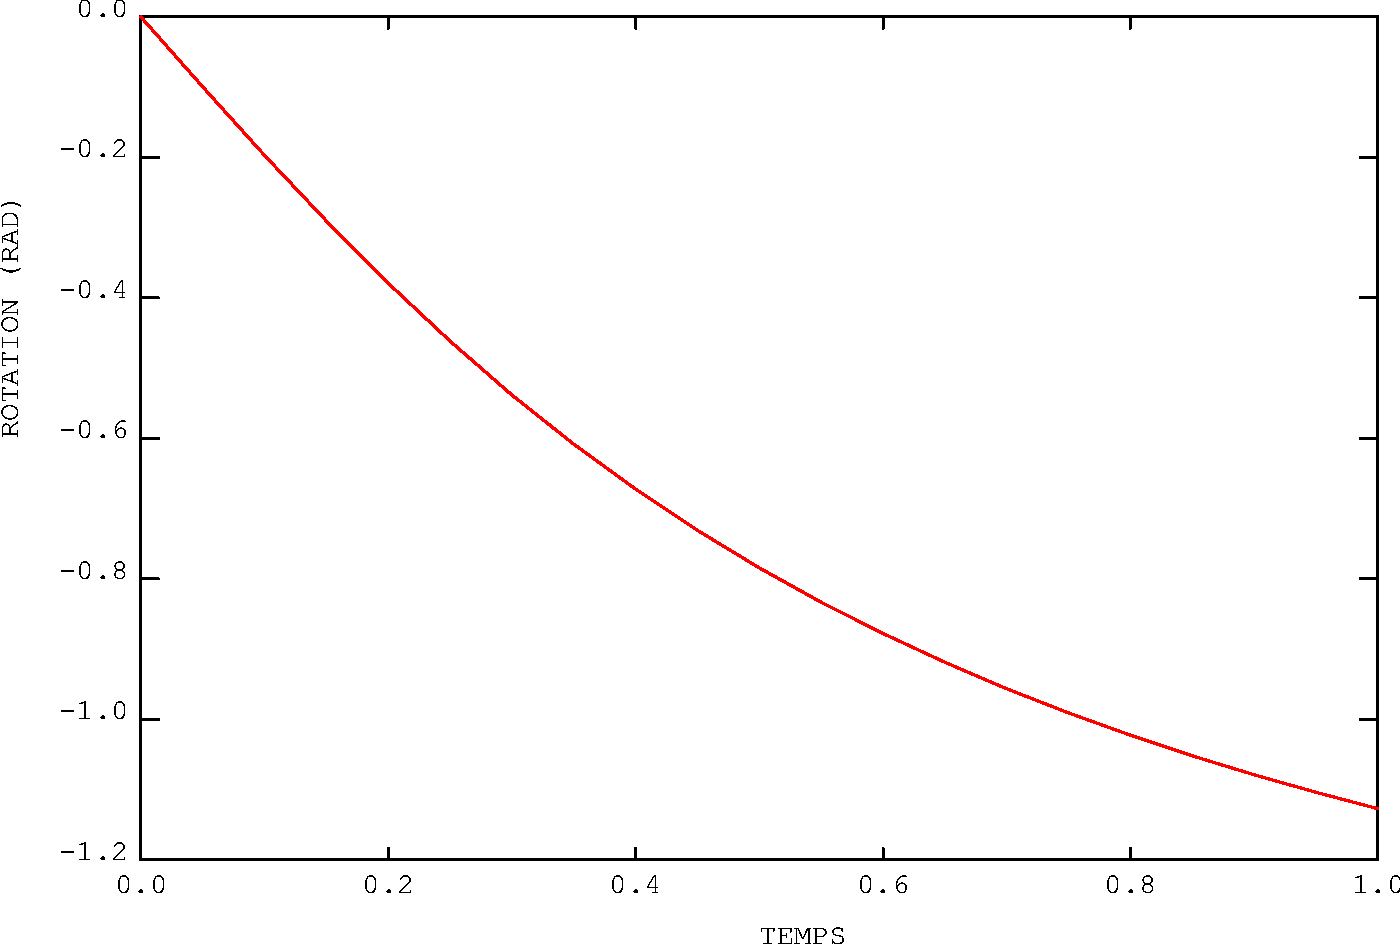
\includegraphics[height=3.5cm]{images/exo/exo_1_evol}
    \end{textblock*}
    \normalsize
    \item<2-> \fe{\red{Problème : l'effort est calculé sur la configuration initiale et n'est pas mis à jour}}
                 {\red{Problem: the force is calculated on the initial shape and not updated}}
    \item<2-> \fe{\green{Objectif : \g{mettre à jour la direction de l'effort} au cours du calcul}}
                 {\green{Purpose: \g{update the force direction} during the calculation}}
    \begin{center}
      \fe{\avous{~À vous de jouer !}}{\avous{~It's up to you!}}
    \end{center}
  \end{itemize}
\end{frame}
}

{\setbeamerfont{framesubtitle}{size=\tiny}
\begin{frame}{\fe{Exercice 1 : poutre avec force suiveuse}{Exercise 1: beam with following force}}
             {\url{https://www-cast3m.cea.fr/index.php?page=exemples&exemple=formation_pasapas_1_initial}}
  \begin{itemize}
    \item \fe{Quelques objets utiles}{Some useful objects}\\
    \small
    \kw{p2 } \fe{point au sommet de la poutre, où est appliqué la force}{point at the top of the beam, where the force is prescribed}\\
    \kw{ev1} \fe{évolution de l'amplitude de la force à appliquer vs. temps}{force magnitude to be applied as a function of time}
    \normalsize
    \item \fe{Quelques opérateurs utiles}{Some useful operators}\\
    \small
    \kwr{EXTR} \fe{pour extraire des valeurs d'un champ}{to extract values from a field}\\
    \kwr{COS SIN} \fe{pour faire un peu de trigonométrie}{for a bit of trigonometry}\\
    \kwr{IPOL} \fe{pour interpoler l'amplitude de la force à l'instant de calcul}
                  {to interpolate the force magnitude at the current time step}\\
    \kwr{FORC} \fe{pour appliquer une force ponctuelle}{to apply a point force}
    \normalsize
    \item \fe{Quelques indices utiles de la table}{Some useful table indices}\\
    \small
    \kwg{'ESTIMATION'.'DEPLACEMENTS'} \fe{dernier champ de déplacement convergé}{last converged displacement field}
    \kwg{'WTABLE'.'CHARGEMENT'} \fe{chargement courant}{current load}
    \normalsize
  \end{itemize}
\end{frame}
}

\begin{frame}{\fe{Exercice 1 : poutre avec force suiveuse}{Exercise 1: beam with following force}}
             {\fe{Solution avec PERSO1}{Solution with PERSO1}}
  \footnotesize
  \begin{itemize}
    \item \fe{Utiliser la procédure \kwv{PERSO1} \red{(1 appel / pas de temps)} pour mettre à jour la force\\
              sur la configuration déformée au \tou{début du pas (explicite)}}
             {Use procedure \kwv{PERSO1} \red{(1 call / time step)} to update the force on deformed shape\\
              at \tou{beginning of time step (explicit)}}
    \item \fe{Créer un objet CHARGEMEnt et écraser \kwg{'WTABLE' . 'CHARGEMENT'}}
             {Create an load (CHARGEMEnt object) and overwrite \kwg{'WTABLE' . 'CHARGEMENT'}}
  \end{itemize}
  \vspace{4.5cm}
  \scriptsize
  \begin{textblock*}{10cm}(0.3cm,-4.2cm)
    \fe{\emph{Programme principal}}{\emph{Main program}}
    \lstinputlisting[basicstyle=\ttfamily\tiny, language=gibiane, firstline=87, lastline=90]{dgibi/formation_pasapas_1_solution.dgibi}
  \end{textblock*}
  \begin{textblock*}{10cm}(6.3cm,-4.2cm)
    \fe{\emph{\violet{Procédure PERSO1}}}{\emph{\violet{PERSO1 procedure}}}
    \lstinputlisting[basicstyle=\ttfamily\tiny, language=gibiane, firstline=47, lastline=60]{dgibi/formation_pasapas_1_solution.dgibi}
  \end{textblock*}
\end{frame}

\begin{frame}{\fe{Exercice 1 : poutre avec force suiveuse}{Exercise 1: beam with following force}}
             {\fe{Solution avec PERSO1}{Solution with PERSO1}}
  \small
  \begin{itemize}
    \item \fe{Résultats}{Results}\\
    \scriptsize
    \fe{base encastrée, force \tou{perpendiculaire} à la poutre, déplacement "important"}
       {clamped base, force \tou{perpendicular} to the beam, "large" displacement}\\
    \begin{tikzpicture}
      \draw [-,thick] (0,0) -- (0,3);
      \draw [->, red] (0,3) -- (0.5,3) node (force) [right, red] {$F$};
      \draw [-]       (-0.2,0) -- (0.25,0);
      \draw [-]       (-0.2,-0.1) -- (-0.1,0);
      \draw [-]       (-0.1,-0.1) -- (0,0);
      \draw [-]       (0,-0.1) -- (0.1,0);
      \draw [-]       (0.1,-0.1) -- (0.2,0);
    \end{tikzpicture}
    \hspace{0.9cm}
    \animategraphics[controls,loop,poster=last,height=3cm]{10}{images/exo/exo_1_solu_deformee.}{01}{21}
    \begin{textblock*}{10cm}(8cm,-3.5cm)
      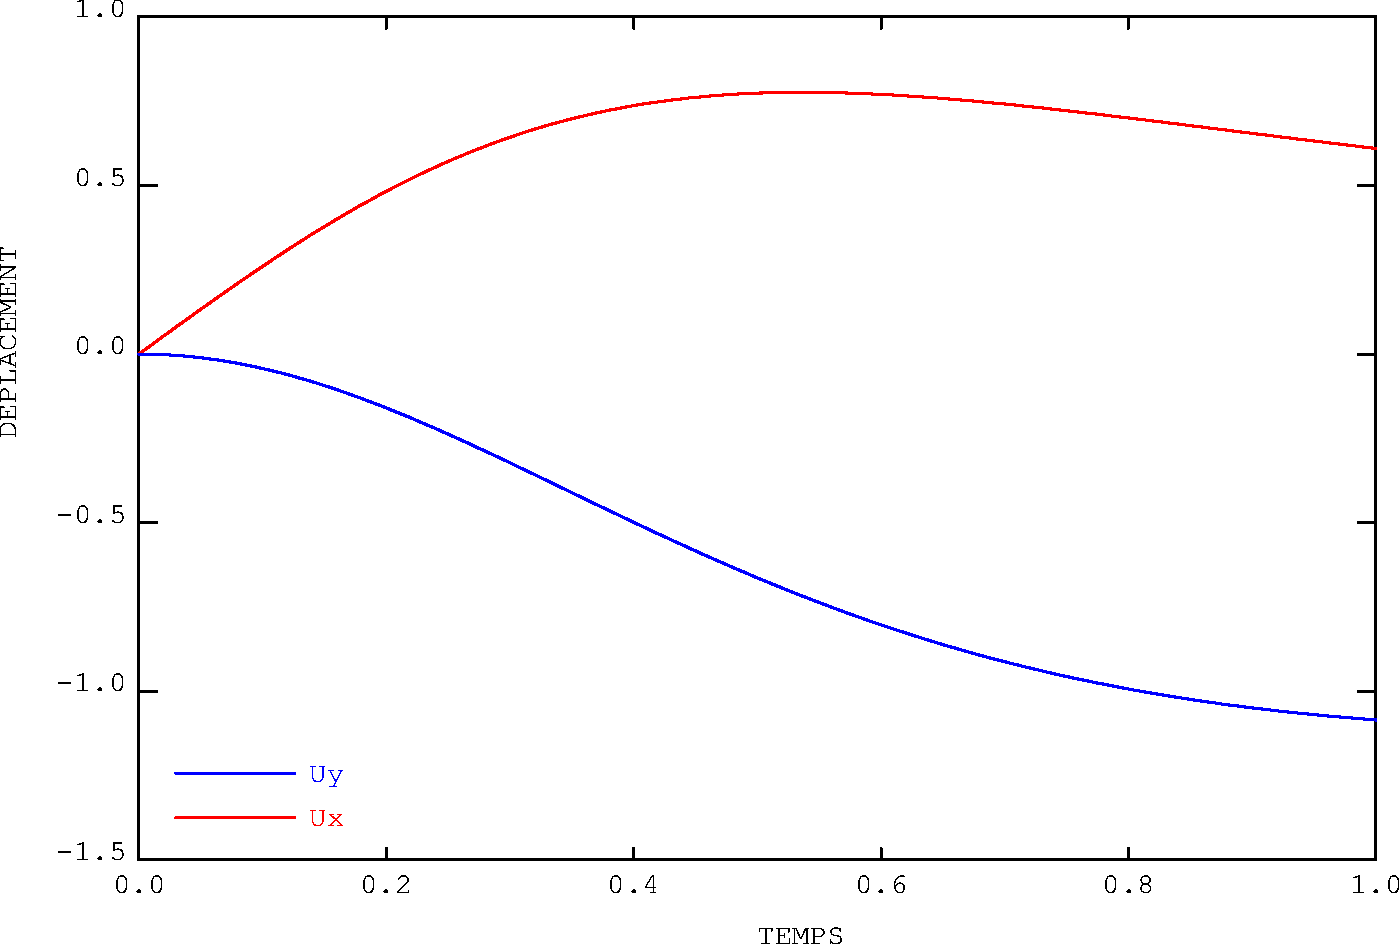
\includegraphics[height=3cm]{images/exo/exo_1_solu_evol}
    \end{textblock*}
    \normalsize
  \end{itemize}
\end{frame}

\begin{frame}{\fe{Exercice 1 : poutre avec force suiveuse}{Exercise 1: beam with following force}}
             {\fe{Solution (bis) avec CHARMECA}{Solution (bis) with CHARMECA}}
  \footnotesize
  \begin{itemize}
    \item \fe{Idem mais avec la procédure \kwv{CHARMECA}, pour mettre à jour la force\\
              sur la configuration déformée au \tou{début du pas (explicite)}}
             {Idem but with the \kwv{CHARMECA} procedure, to update the force on deformed shape\\
              at \tou{beginning of time step (explicit)}}
    \item \fe{Plus besoin de CHARGEMEnt initial}{No need for initial load (CHARGEMEnt object)}
    \item \fe{\red{Plus long (1 appel / itération / pas de temps)} et \green{résultats identiques}}
             {\red{Longer (1 call / each iteration / time step)} and \green{results are identical}}
  \end{itemize}
  \vspace{4.5cm}
  \scriptsize
  \begin{textblock*}{10cm}(0.3cm,-4.3cm)
    \fe{\emph{Programme principal}}{\emph{Main program}}
    \lstinputlisting[basicstyle=\ttfamily\tiny, language=gibiane, firstline=136, lastline=140]{dgibi/formation_pasapas_1_solution.dgibi}
  \end{textblock*}
  \begin{textblock*}{10cm}(6.3cm,-4.3cm)
    \fe{\emph{\violet{Procédure CHARMECA}}}{\emph{\violet{CHARMECA procedure}}}
    \lstinputlisting[basicstyle=\ttfamily\tiny, language=gibiane, firstline=63, lastline=77]{dgibi/formation_pasapas_1_solution.dgibi}
  \end{textblock*}
\end{frame}

\begin{frame}{\fe{Exercice 1 : poutre avec force suiveuse}{Exercise 1: beam with following force}}
             {\fe{Solution (ter) avec CHARMECA}{Solution (ter) with CHARMECA}}
  \footnotesize
  \begin{itemize}
    \item \fe{Idem mais avec la procédure \kwv{CHARMECA}, pour mettre à jour la force\\
              sur la configuration déformée à la \tou{fin du pas (implicite)}}
             {Idem but with the \kwv{CHARMECA} procedure, to update the force on deformed shape\\
              at the \tou{end of time step (implicit)}}
    \item \fe{Attention : peut être instable !}{Watch out: can become unstable!}
  \end{itemize}
  \vspace{4.5cm}
  \scriptsize
  \begin{textblock*}{10cm}(0.3cm,-4.4cm)
    \fe{\emph{Programme principal}}{\emph{Main program}}
    \lstinputlisting[basicstyle=\ttfamily\tiny, language=gibiane, firstline=136, lastline=140]{dgibi/formation_pasapas_1_solution.dgibi}
  \end{textblock*}
  \begin{textblock*}{10cm}(6.3cm,-4.4cm)
    \fe{\emph{\violet{Procédure CHARMECA}}}{\emph{\violet{CHARMECA procedure}}}
    \lstinputlisting[basicstyle=\ttfamily\tiny, language=gibiane, firstline=142, lastline=159]{dgibi/formation_pasapas_1_solution.dgibi}
  \end{textblock*}
\end{frame}

{\setbeamerfont{framesubtitle}{size=\tiny}
\begin{frame}{\fe{Exercice 2 : fissuration par suppression d'éléments}
                 {Exercise 2: fracture by elements removal}}
             {\url{https://www-cast3m.cea.fr/index.php?page=exemples&exemple=formation_pasapas_2_initial}}
  \small
  \begin{itemize}
    \item \fe{Plaque en traction \textcolor{green}{(déplacements imposés)}}
             {Plate under tension \textcolor{green}{(imposed displacements)}}\\
    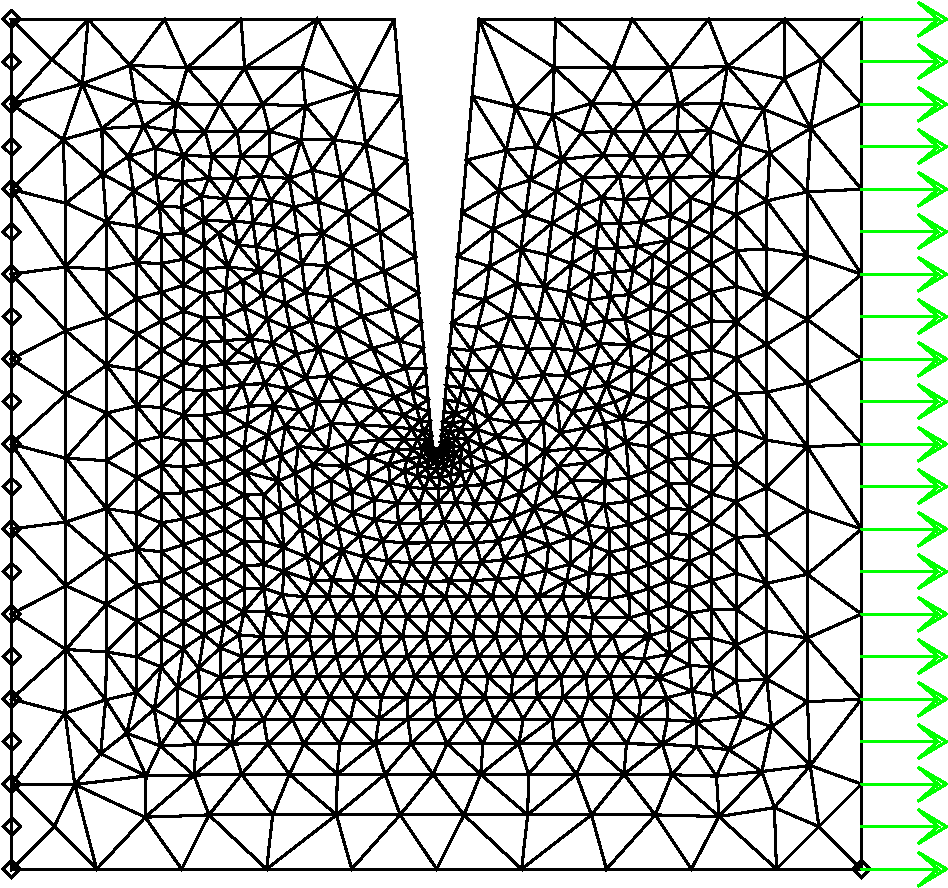
\includegraphics[height=3cm]{images/exo/exo_2_chargement} \hspace{0.2cm}
    \animategraphics[controls,loop,poster=last,height=3.5cm]{7}{images/exo/exo_2_sigma.}{01}{11} \hspace{0.2cm}
    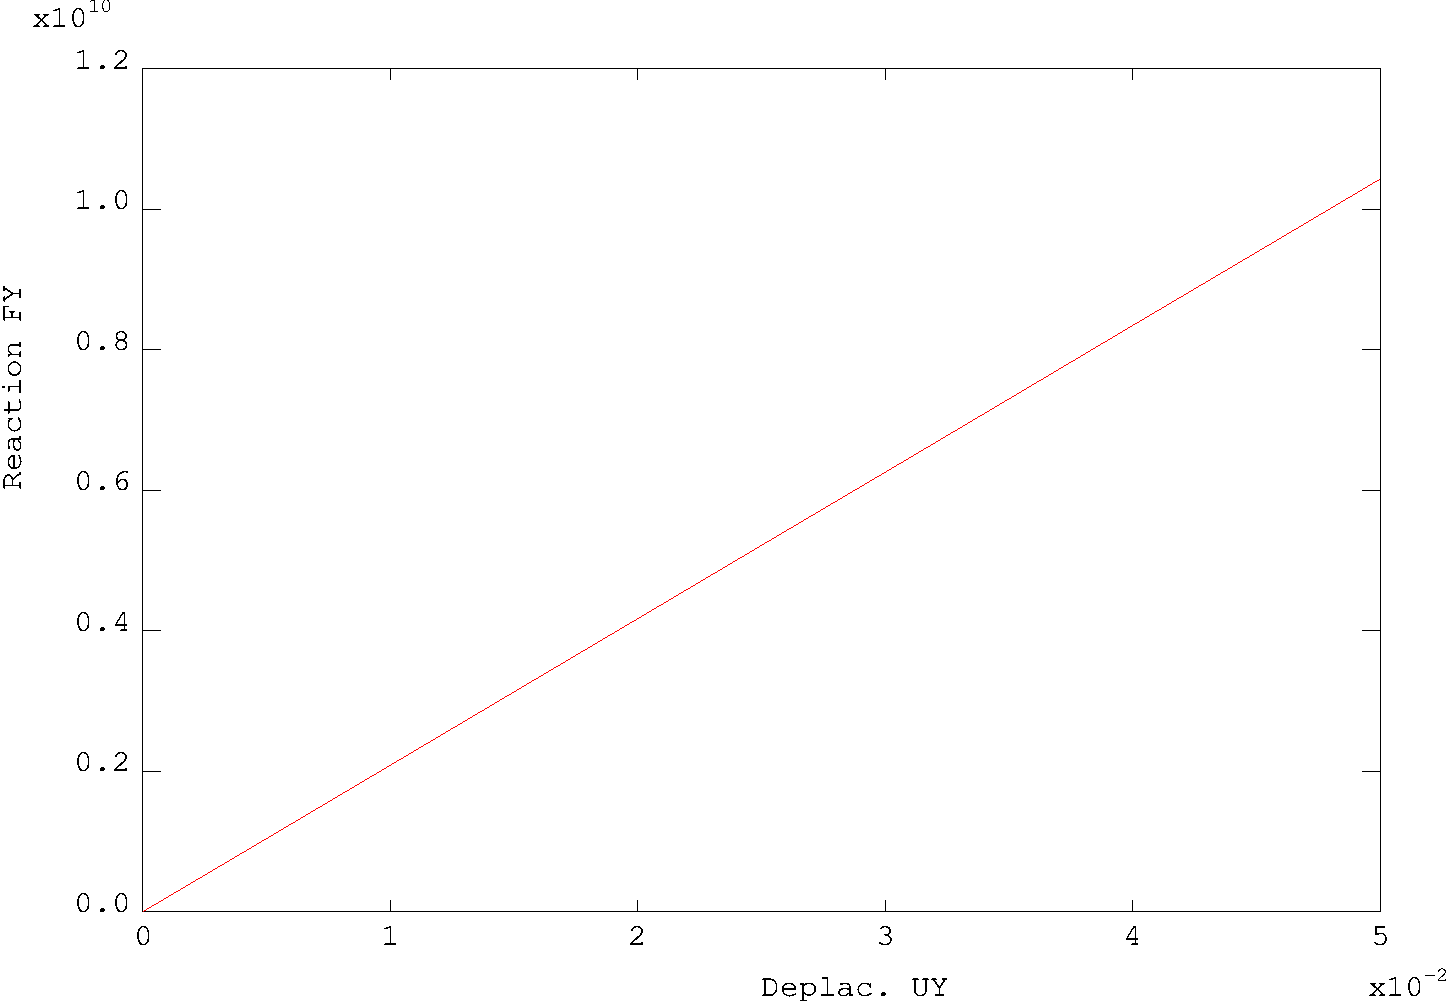
\includegraphics[height=3cm]{images/exo/exo_2_evol}
    \item<2-> \fe{\green{Objectif : \g{supprimer les éléments} au cours du calcul}\\
                  On utilisera un critère de rupture simple sur la 1ère contrainte principale :
                  \begin{center}
                    rupture si $\sigma_I \geq$ 22~GPa\\ \avous{~À vous de jouer !}
                  \end{center}}
                 {\green{Purpose: \g{remove the elements} during calculations}\\
                  We will use a simple fracture criterion based on the 1st principal stress:
                  \begin{center}
                    fracture if $\sigma_I \geq$ 22~GPa\\ \avous{~It's up to you!}
                  \end{center}}
  \end{itemize}
\end{frame}
}

{\setbeamerfont{framesubtitle}{size=\tiny}
\begin{frame}{\fe{Exercice 2 : fissuration par suppression d'éléments}
                 {Exercise 2: fracture by elements removal}}
             {\url{https://www-cast3m.cea.fr/index.php?page=exemples&exemple=formation_pasapas_2_initial}}
  \begin{itemize}
    \item \fe{Quelques opérateurs utiles}{Some useful operators}\\
    \small
    \kwr{PRIN} \fe{calcul des contraintes principales}{compute principal stresses}\\
    \kwr{ELEM} \fe{séléction des éléments où un champ vérifie une condition}{select the elements of a field that meets a criteria}\\
    \kwr{REDU} \fe{réduction d'un modèle sur un sous maillage}{reduction of a model on a sub part of a mesh}\\
    \kwr{CHAN} \fe{changement des points support d'un champ}{change the support points of a field}
    \normalsize
    \item \fe{Quelques indices utiles de la table}{Some useful table indices}\\
    \small
    \kwg{ESTIMATION}\kw{.}\kwg{CONTRAINTES} \fe{dernier champ de contraintes convergé}{last converged stress field}
    \kwg{WTABLE}\kw{.}\kwg{MODELE} \fe{modèle courant}{current model}\\
    \kwg{WTABLE}\kw{.}\kwg{CARACTERISTIQUES} \fe{paramètres matériau}{material properties}
    \normalsize
  \end{itemize}
\end{frame}
}

\begin{frame}{\fe{Exercice 2 : fissuration par suppression d'éléments}
                 {Exercise 2: fracture by elements removal}}
             {\fe{Solution avec PERSO1}{Solution with PERSO1}}
  \footnotesize
  \begin{itemize}
    \small
    \item \fe{Utiliser la procédure \kwv{PERSO1}}{Use procedure \kwv{PERSO1}}
    \item \fe{Extraire le modèle et les contraintes dans \kwg{ESTIMATION}}{Extract the model and stress field in \kwg{ESTIMATION}}
    \item \fe{Calculer la contrainte principale $\sigma_I$}{Compute the 1st principal stress $\sigma_I$}
    \item \fe{Extraire les éléments "intacts"}{Extract the "intact" elements}
    \item \fe{Réduire le modèle sur ce maillage et écraser \kwg{WTABLE}\kw{.}\kwg{MODELE}}
             {Reduce the model on this mesh and overwrite \kwg{WTABLE}\kw{.}\kwg{MODELE}}
    \item \fe{Réduire les pas de temps}{Reduce time steps}
  \end{itemize}
  \vspace{4.5cm}
  \scriptsize
  \begin{textblock*}{10cm}(0.3cm,-3.2cm)
    \fe{\emph{Programme principal}}{\emph{Main program}}
    \lstinputlisting[basicstyle=\ttfamily\tiny, language=gibiane, firstline=92, lastline=95]{dgibi/formation_pasapas_2_solution.dgibi}
  \end{textblock*}
  \begin{textblock*}{10cm}(6.2cm,-4cm)
    \fe{\emph{\violet{Procédure PERSO1}}}{\emph{\violet{PERSO1 procedure}}}
    \lstinputlisting[basicstyle=\ttfamily\tiny, language=gibiane, firstline=75, lastline=84]{dgibi/formation_pasapas_2_solution.dgibi}
  \end{textblock*}
\end{frame}

\begin{frame}{\fe{Exercice 2 : fissuration par suppression d'éléments}
                 {Exercise 2: fracture by elements removal}}
             {\fe{Solution avec PERSO1}{Solution with PERSO1}}
  \footnotesize
  \begin{itemize}
    \item \fe{Résultats}{Results}\\
    \hspace{1cm}
    \animategraphics[controls,loop,poster=last,height=4.5cm]{7}{images/exo/exo_2_solu_sigma.}{01}{47} \hspace{1.5cm}
    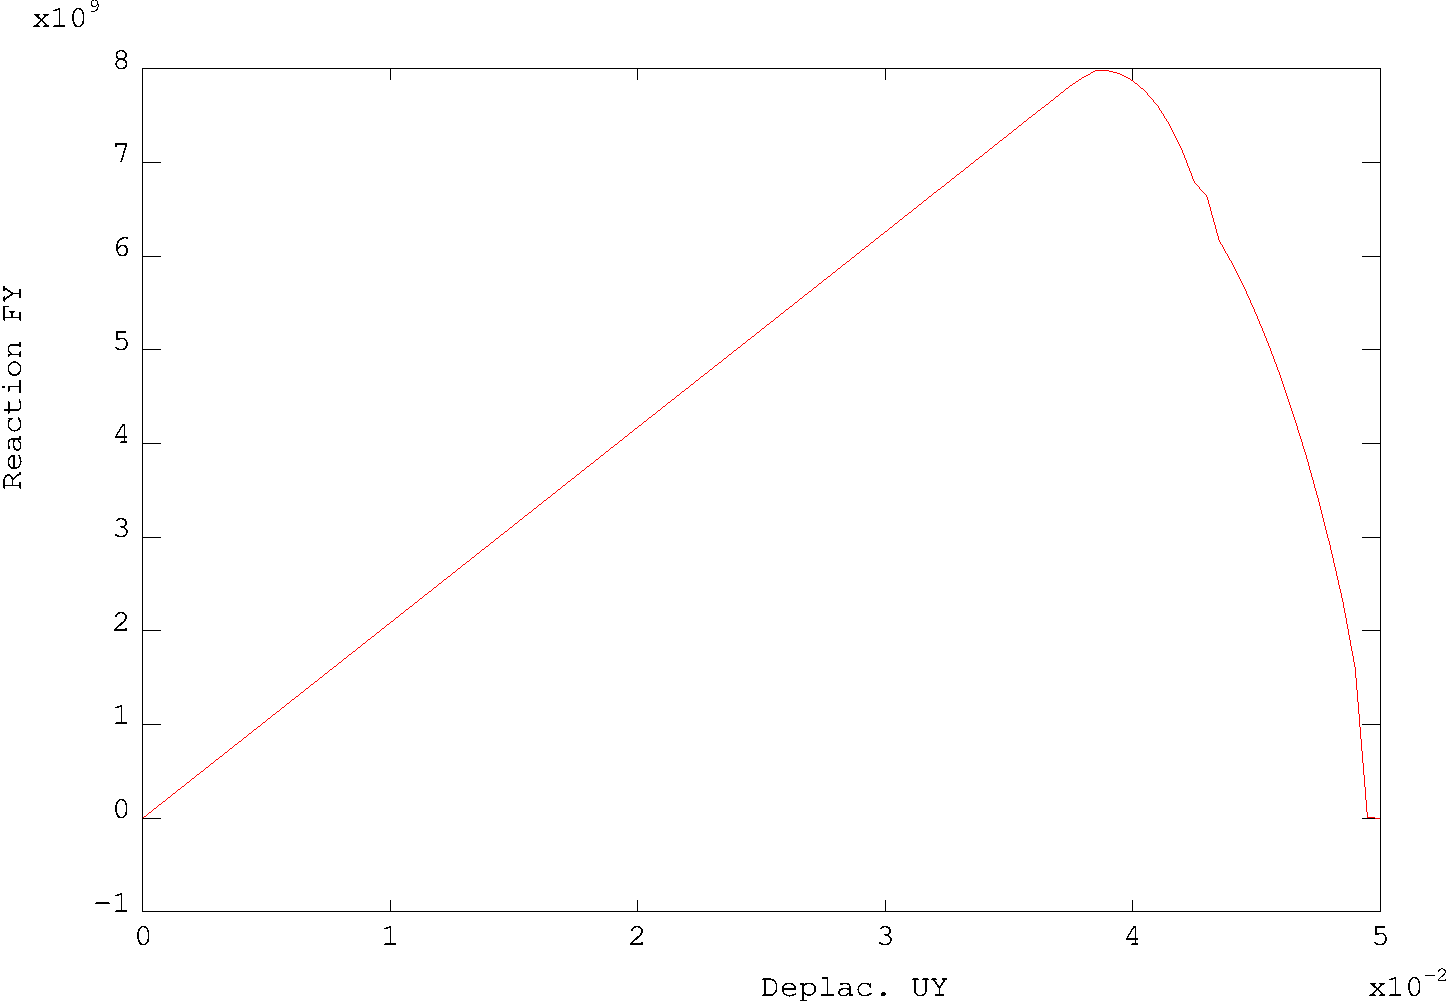
\includegraphics[height=3.5cm]{images/exo/exo_2_solu_evol}
    \item \fe{Modèle peu robuste\\ résultats très sensibles à la discrétisation espace/temps}
             {Undependable model\\ results quite sensitive to time/space discretization}
  \end{itemize}
\end{frame}

\begin{frame}{\fe{Exercice 2 : fissuration par suppression d'éléments}
                 {Exercise 2: fracture by elements removal}}
             {\fe{Solution (bis) avec PERSO1}{Solution (bis) with PERSO1}}
  \footnotesize
  \begin{itemize}
    \item \fe{Idem mais sur les \g{\red{blocages}}}{Idem but on the \g{\red{boundary conditions}}}
    \item \fe{Écraser \kwg{WTABLE}\kw{.}\kwg{BLOCAGES\_MECANIQUES}}{Overwrite \kwg{WTABLE}\kw{.}\kwg{BLOCAGES\_MECANIQUES}}
    \item \fe{Activer l'option \kwg{GRANDS\_DEPLACEMENTS}}{Use option \kwg{GRANDS\_DEPLACEMENTS}}
  \end{itemize}
  \vspace{4.5cm}
  \scriptsize
  \begin{textblock*}{10cm}(0.3cm,-3.2cm)
    \fe{\emph{Programme principal}}{\emph{Main program}}
    \lstinputlisting[basicstyle=\ttfamily\tiny, language=gibiane, firstline=100, lastline=104]{dgibi/formation_pasapas_2_solution_bis.dgibi}
  \end{textblock*}
  \begin{textblock*}{10cm}(5.8cm,-4.3cm)
    \fe{\emph{\violet{Procédure PERSO1}}}{\emph{\violet{PERSO1 procedure}}}
    \lstinputlisting[basicstyle=\ttfamily\tiny, language=gibiane, firstline=75, lastline=92]{dgibi/formation_pasapas_2_solution_bis.dgibi}
  \end{textblock*}
\end{frame}

\begin{frame}{\fe{Exercice 2 : fissuration par suppression d'éléments}
                 {Exercise 2: fracture by elements removal}}
             {\fe{Solution (bis) avec PERSO1}{Solution (bis) with PERSO1}}
  \footnotesize
  \begin{itemize}
    \item \fe{Résultats}{Results}\\
    \hspace{1cm}
    \animategraphics[controls,loop,poster=last,height=4.5cm]{7}{images/exo/exo_2_solu_bis_sigma.}{01}{47} \hspace{1.5cm}
    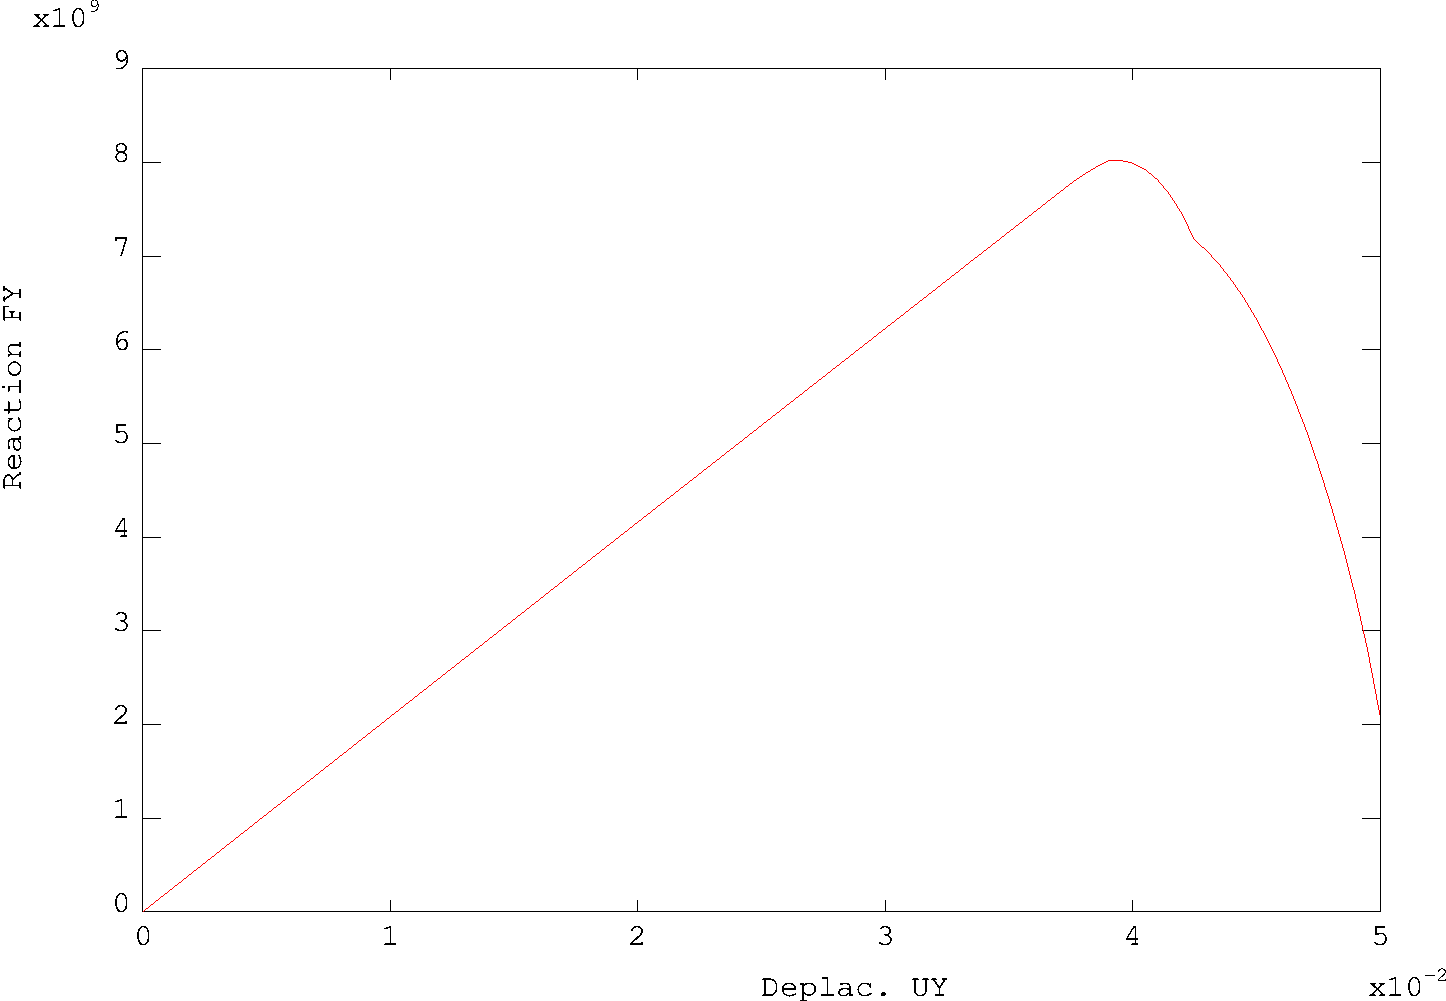
\includegraphics[height=3.5cm]{images/exo/exo_2_solu_bis_evol}
    \item \fe{Modèle peu robuste\\ résultats très sensibles à la discrétisation espace/temps}
             {Undependable model\\ results quite sensitive to time/space discretization}
  \end{itemize}
\end{frame}

%%%%%%%%%%%%%%%%%%%%%%%%%%%%%%%%%%%%%%%%%%%%%%%%%%%%%%%%%%
\fe{\section{Solveur thermique}}{\section{Thermal solver}}
\label{thermique}
%%%%%%%%%%%%%%%%%%%%%%%%%%%%%%%%%%%%%%%%%%%%%%%%%%%%%%%%%%

\fe{\subsection{Théorie}}{\subsection{Theory}}
\label{thermique_theorie}

\begin{frame}{\fe{Solveur thermique}{Thermal solver}}
             {\fe{Rappel des équations}{Reminder on equations}}
  \begin{itemize}
    \item<1->[] \fe{Équations locales du problème transitoire}
                   {Local equations of the transient problem}\\
    \scriptsize
    \fe{\begin{tabular}{lll}
          équation de la chaleur & $\rho c_p \frac{\partial T}{\partial t}+\tx{div}\underbrace{(-\lambda \tx{grad}T)}_{\phi}-q=0$ & sur $V$ \\
          flux imposé            & $\phi.n = \phi_{\tx{imp}} + \underbrace{h(T_f-T)}_{convection}
                                                             + \underbrace{\varepsilon\sigma(T^4_{\infty}-T^4)}_{rayonnement}$    & sur $\partial V_{\phi}$ \\
          température imposée    & $T = T_{\tx{imp}}$                                                                             & sur $\partial V_{T}$ \\
        \end{tabular}}
       {\begin{tabular}{lll}
        heat equation            & $\rho c_p \frac{\partial T}{\partial t}+\tx{div}\underbrace{(-\lambda \tx{grad}T)}_{\phi}-q=0$ & on $V$ \\
        imposed heat flow        & $\phi.n = \phi_{\tx{imp}} + \underbrace{h(T_f-T)}_{convection}
                                                             + \underbrace{\varepsilon\sigma(T^4_{\infty}-T^4)}_{radiation}$      & on $\partial V_{\phi}$ \\
        imposed temperature      & $T = T_{\tx{imp}}$                                                                             & on $\partial V_{T}$ \\
    \end{tabular}}
    \normalsize
    \onslide<2->{
    \begin{block}{\fe{Formulation faible et discrétisée :}
                     {Weak and discrete formulation:}}
      \begin{equation*}
        [C]\{\dot{T}\}+[K]\{T\}=\{P\}
      \end{equation*}
    \end{block}~\\
    \scriptsize
    \fe{avec les matrices :}{with the matrices:}
    \begin{tabular}{lll}~\\
      $[C]=\int_V\rho c_p [N]^T[N]dV$                                     & \fe{matrice de capacité}{capacity matrix}         & \kwr{CAPA}\\
      $[K]=\int_V[B]^T[\lambda][B]dV+\int_{\partial V_{\phi}}h[N]^T[N]dS$ & \fe{matrice de conductivité}{conductivity matrix} & \kwr{COND}
     \end{tabular}~\\~\\
    \fe{et le vecteur chargement nodal équivalent (\kwr{SOUR FLUX CONV} \kwo{PAS\_RAYO}) :}
       {and the equivalent nodal load vector (\kwr{SOUR FLUX CONV} \kwo{PAS\_RAYO}):}\\
      $\{P\}=\int_V[N]^T\{q\}_{\tx{imp}}dV+\int_{\partial V_{\phi}}[N]^T(\{\phi\}_{\tx{imp}}+h\{T\}_f+\varepsilon\sigma(\{T\}_\infty^4-\{T\}^4))dS$}
  \end{itemize}
  \normalsize
\end{frame}

\begin{frame}{\fe{Solveur thermique}{Thermal solver}}
  \begin{itemize}
    \item[]
    \begin{block}{\fe{Discrétisation temporelle avec un $\theta$-schéma}{Time discretization with a $\theta$-scheme}}
      \begin{equation*}
        [C]_{\star}\frac{\red{\{T\}_1}-\green{\{T\}_0}}{\Delta t}+[K]_{\star}\{T\}_{\star}=\{P\}_{\star}
      \end{equation*}
    \end{block}~\\
    \footnotesize
    \item[] \fe{Avec :}{With:}\\
    \begin{tabular}{ll}
      $\red{\{T\}_1}$                       & \fe{températures nodales à la fin du pas de temps $\red{t_1}$ (inconnues)}
                                                 {nodal temperatures at end of time step $\red{t_1}$ (unknown)}\\
      $\green{\{T\}_0}$                     & \fe{températures nodales au début du pas de temps $\green{t_0}$ (connues)}
                                                 {nodal temperatures at beginning of time step $\green{t_0}$ (knwown)}\\
      $\Delta t = \red{t_1} - \green{t_0}$  & \fe{le pas de temps}{the time step}
    \end{tabular}~\\~\\
    \item[] \fe{$[C]_{\star}$ $[K]_{\star}$ et $\{P\}_{\star}$ sont évalués :}{$[C]_{\star}$ $[K]_{\star}$ and $\{P\}_{\star}$ are estimated:}\\
    \begin{tabular}{ll}
      \fe{au temps}{at time}                & $t_{\star}     = \theta \red{t_1} + (1-\theta) \green{t_0}$\\
      \fe{à la température}{at temperature} & $\{T\}_{\star} = \theta \red{\{T\}_1} + (1-\theta) \green{\{T\}_0}$
    \end{tabular}~\\~\\
    \item[] \fe{$\theta$ est le \g{coefficient de relaxation} de ce schéma, entre 0 et 1}
               {$\theta$ is the \g{relaxation coefficient} of this scheme, between 0 and 1}\\
    \begin{tabular}{ll}
      $\theta$               & \fe{réglable via l'indice \kwg{RELAXATION\_THETA}}{adjustable via index \kwg{RELAXATION\_THETA}}\\
      $\theta = 0$           & \fe{schéma explicite}{explicit scheme}\\
      $\theta = \frac{1}{2}$ & \fe{schéma implicite de Crank-Nicolson}{implicit Crank-Nicolson scheme}\\
      $\theta = 1$           & \fe{schéma implicite complet (par défaut)}{full implicit scheme (default)}
    \end{tabular}
  \end{itemize}
\end{frame}

\begin{frame}{\fe{Algorithme de TRANSNON}{TRANSNON algorithm}}
  \tiny
  \begin{tikzpicture}[node distance=0.6cm,
    every node/.style={fill=white}, align=center]
  % Cellules (style, position, contenu)
  \fe{\node (ini)   [bstep] {Initialisations\\ \kwv{CHARTHER}};}
     {\node (ini)   [bstep] {Initializations\\ \kwv{CHARTHER}};}
  \fe{\node (ini0)  [note, right of=ini, xshift=1.5cm, anchor=west] {Lecture des options, unités (°C ou K), état initial \kwo{PAS\_MODL},\\
                                                                     calcul des facteurs de forme (rayonnement)  \kwo{PAS\_RAYO} \dots};}
     {\node (ini0)  [note, right of=ini, xshift=1.5cm, anchor=west] {Option reading, units (°C or K), initial state \kwo{PAS\_MODL},\\
                                                                     view factors (for radiation) \kwo{PAS\_RAYO} \dots};}

  \fe{\node (ins)   [gstep, below of=ini, yshift=-0.5cm] {État à $\green{\{T\}_0}$,$t_{\star}$\\
                                                         \kwv{PARATHER}\\
                                                         M.à.j. matériau, $[K]_{\star}$ et $[C]_{\star}$\\
                                                         \kwo{PAS\_RAYO}, \kwv{CHARTHER}, $\{P\}_{\star}$};}
     {\node (ins)   [gstep, below of=ini, yshift=-0.5cm] {State at $\green{\{T\}_0}$,$t_{\star}$\\
                                                          \kwv{PARATHER}\\
                                                          Material updating, $[K]_{\star}$ et $[C]_{\star}$\\
                                                          \kwo{PAS\_RAYO}, \kwv{CHARTHER}, $\{P\}_{\star}$};}
  \fe{\node (ins0)  [note, right of=ins, xshift=1.5cm, anchor=west] {Mise à jour variables externes \kwv{PARATHER} et carac. matériaux,\\
                                                                     Calcul de $[K]_{\star}$ \kwr{COND CONV}, $[C]_{\star}$ \kwr{CAPA} à $\green{\{T\}_0}$ et $t_{\star}$\\
                                                                     Calcul de $\{P\}_{\star}$ \kwr{TIRE} à $\green{\{T\}_0}$ et $t_{\star}$\\
                                                                     Ajout des termes de rayonnement \kwo{PAS\_RAYO}\\
                                                                     On définit alors l'\g{opérateur} $[L]_{\star}=\frac{1}{\Delta t}[C]_{\star}+\theta[K]_{\star}$};}
     {\node (ins0)  [note, right of=ins, xshift=1.5cm, anchor=west] {Updating external variables \kwv{PARATHER} and material parameters,\\
                                                                     Calculation of $[K]_{\star}$ \kwr{COND CONV}, $[C]_{\star}$ \kwr{CAPA} at $\green{\{T\}_0}$ and $t_{\star}$\\
                                                                     Calculation of $\{P\}_{\star}$ \kwr{TIRE} at $\green{\{T\}_0}$ and $t_{\star}$\\
                                                                     Adding the radiative terms \kwo{PAS\_RAYO}\\
                                                                     We define the \g{operator} $[L]_{\star}=\frac{1}{\Delta t}[C]_{\star}+\theta[K]_{\star}$};}

  \fe{\node (acc)  [rstep, below of=ins, yshift=-0.5cm] {Accélération convergence};}
     {\node (acc)  [rstep, below of=ins, yshift=-0.5cm] {Convergence acceleration};}

      \node (res)  [rstep, below of=acc, yshift=-0.4cm] {\kwr{RESO}};
  \fe{\node (res0) [note, right of=res, xshift=1.5cm, anchor=west] {Calcul incrément de température : $\Delta \{T\}^{i+1} = [L]_{\star}^{-1}\{P\}_{\star}$\\
                                                                    on déduit $\red{\{T\}_1^{i+1}}=\green{\{T\}_0}+\Delta \{T\}^{i+1}$\\
                                                                    et aussi $\{T\}_{\star}^{i+1} = \theta \red{\{T\}_1^{i+1}} + (1-\theta) \green{\{T\}_0}$};}
     {\node (res0) [note, right of=res, xshift=1.5cm, anchor=west] {Temperature increment calculation: $\Delta \{T\}^{i+1} = [L]_{\star}^{-1}\{P\}_{\star}$\\
                                                                    so we get $\red{\{T\}_1^{i+1}}=\green{\{T\}_0}+\Delta \{T\}^{i+1}$\\
                                                                    and also $\{T\}_{\star}^{i+1} = \theta \red{\{T\}_1^{i+1}} + (1-\theta) \green{\{T\}_0}$};}

  \fe{\node (con)  [rtest, below of=res, yshift=-0.6cm] {Convergence ?};}
     {\node (con)  [rtest, below of=res, yshift=-0.6cm] {Convergence?};}
  \fe{\node (con0) [note, right of=con, xshift=1.5cm, anchor=west] {Test sur la \g{variation d'incrément de température}\\ entre 2 itérations successives\\
                                                                    \kwr{MAX}~\kwg{ABS} $\frac{\Delta \{T\}^{i+1}-\Delta \{T\}^i}{\red{\{T\}_1^{i+1}}} <$ \kwg{PRECISION}};}
     {\node (con0) [note, right of=con, xshift=1.5cm, anchor=west] {Test on the \g{temperature increment variation}\\ between 2 successive iterations\\
                                                                    \kwr{MAX}~\kwg{ABS} $\frac{\Delta \{T\}^{i+1}-\Delta \{T\}^i}{\red{\{T\}_1^{i+1}}} <$ \kwg{PRECISION}};}

  \fe{\node (maj)  [rstep, left of=res, xshift=-1.7cm] {État à $\{T\}_{\star}^{i+1}$,$t_{\star}$\\
                                                        \kwv{PARATHER}\\
                                                        M.à.j. matériau\\
                                                        \kwo{PAS\_RAYO}, \kwv{CHARTHER}, $\{P\}_{\star}$};}
     {\node (maj)  [rstep, left of=res, xshift=-1.7cm] {State at $\{T\}_{\star}^{i+1}$,$t_{\star}$\\
                                                        \kwv{PARATHER}\\
                                                        Material updating \\
                                                        \kwo{PAS\_RAYO}, \kwv{CHARTHER}, $\{P\}_{\star}$};}
  
      \node (per)  [gstep, below of=con, yshift=-0.3cm] {\kwv{PERSO2}};

  \fe{\node (tim)  [gtest, below of=per, yshift=-0.4cm] {Fin des pas\\ de temps ?};}
     {\node (tim)  [gtest, below of=per, yshift=-0.4cm] {End of\\ time steps?};}

  \fe{\node (fin)   [bstep, right of=tim, xshift=2cm] {Fin};}
     {\node (fin)   [bstep, right of=tim, xshift=2cm] {End};}

  % Connections entre les cellules
  \draw[->]               (ini) -- (ins);
  \draw[->, draw=Green]   (ins) -- (acc);
  \draw[->, draw=red]     (acc) -- (res);
  \draw[->, draw=red]     (res) -- (con);
  \fe{\draw[->, draw=red]   (con.west) -| node[near start]{non} (maj);}
     {\draw[->, draw=red]   (con.west) -| node[near start]{no}  (maj);}
  \draw[->, draw=red]     (maj) |- (acc);
  \fe{\draw[->, draw=Green] (con) -- node[xshift=0.4cm]{oui} (per);}
     {\draw[->, draw=Green] (con) -- node[xshift=0.4cm]{yes} (per);}
  \draw[->, draw=Green]   (per) -- (tim);
  \fe{\draw[->, draw=Green] (tim.west) -- node[yshift=0.2cm]{non} ++(-2.4,0) -- ++(0,5.2) -- (ins.west);}
     {\draw[->, draw=Green] (tim.west) -- node[yshift=0.2cm]{no}  ++(-2.4,0) -- ++(0,5.2) -- (ins.west);}
  \fe{\draw[->] (tim.east) -- node[yshift=0.2cm]{oui} (fin.west);}
     {\draw[->] (tim.east) -- node[yshift=0.2cm]{yes} (fin.west);}
  \draw[dotted]           (ini) -- (ini0);
  \draw[dotted]           (ins) -- (ins0);
  \draw[dotted]           (res) -- (res0);
  \draw[dotted]           (con) -- (con0);
  \end{tikzpicture}
\end{frame}

\fe{\subsection{Exercices}}{\subsection{Exercises}}
\label{thermique_exo}

{\setbeamerfont{framesubtitle}{size=\tiny}
\begin{frame}{\fe{Exercice 3 : dépendance à la température}
                 {Exercise 3: temperature-dependence}}
             {\url{https://www-cast3m.cea.fr/index.php?page=exemples&exemple=formation_pasapas_3_initial}}
  \small
  \begin{itemize}
    \item \fe{Section carrée chauffée par une source et refroidie par convection}
             {Square section with heat source and cooled by convection}\\
    \tiny
    \begin{tikzpicture}
      \node[anchor=south west,inner sep=0] (image) at (0,0)
      {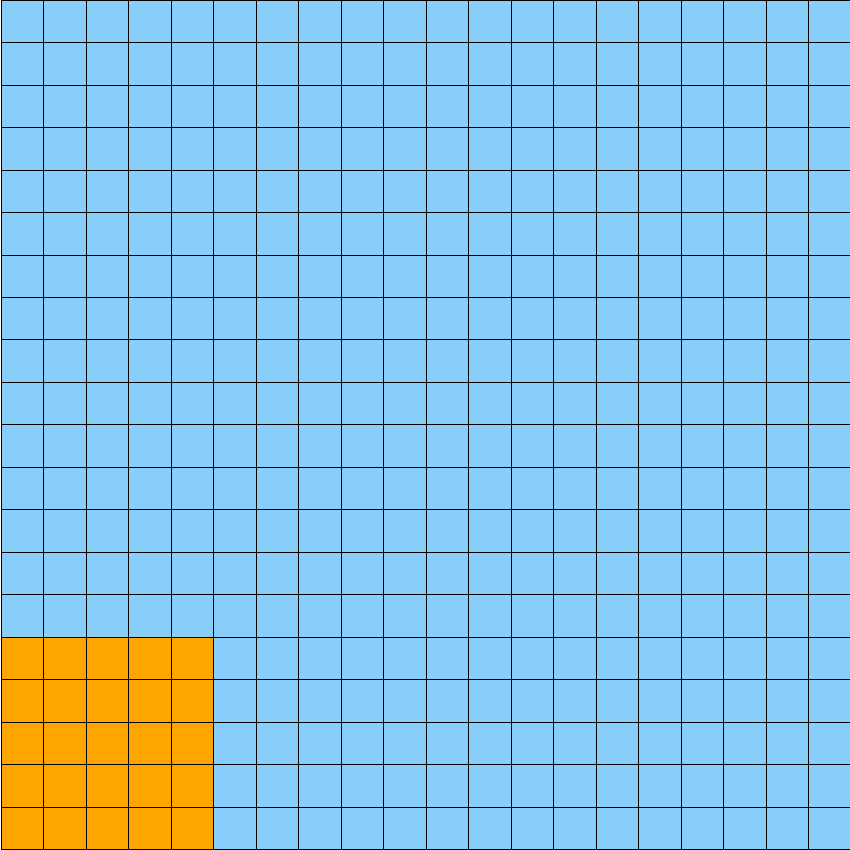
\includegraphics[height=2.5cm]{images/exo/exo_3_maillage}};
      \begin{scope}[x={(image.south east)},y={(image.north west)}]
        \draw (0.12,0.15) node {Source};
        \draw (0.5,0.5) node {$\lambda$~=~317~W/m/K};
        \draw (0.5,0.92) node {$h$~=~150~W/m$^2$/K};
        \draw[-{>[bend]}] (1.1,0.2) arc[radius=0.05, start angle=30, end angle=330];
        \draw[-{>[bend]}] (1.1,0.5) arc[radius=0.05, start angle=30, end angle=330];
        \draw[-{>[bend]}] (1.1,0.8) arc[radius=0.05, start angle=30, end angle=330];
        \draw[-{>[bend]}] (0.2,1.1) arc[radius=0.05, start angle=30, end angle=330];
        \draw[-{>[bend]}] (0.5,1.1) arc[radius=0.05, start angle=30, end angle=330];
        \draw[-{>[bend]}] (0.8,1.1) arc[radius=0.05, start angle=30, end angle=330];
      \end{scope}
    \end{tikzpicture}
    \hspace{0.1cm}
    \if \animation 1
      \animategraphics[controls,loop,poster=last,height=3cm]{7}{images/exo/exo_3_temperature.}{01}{51} \hspace{0.2cm}
    \else
      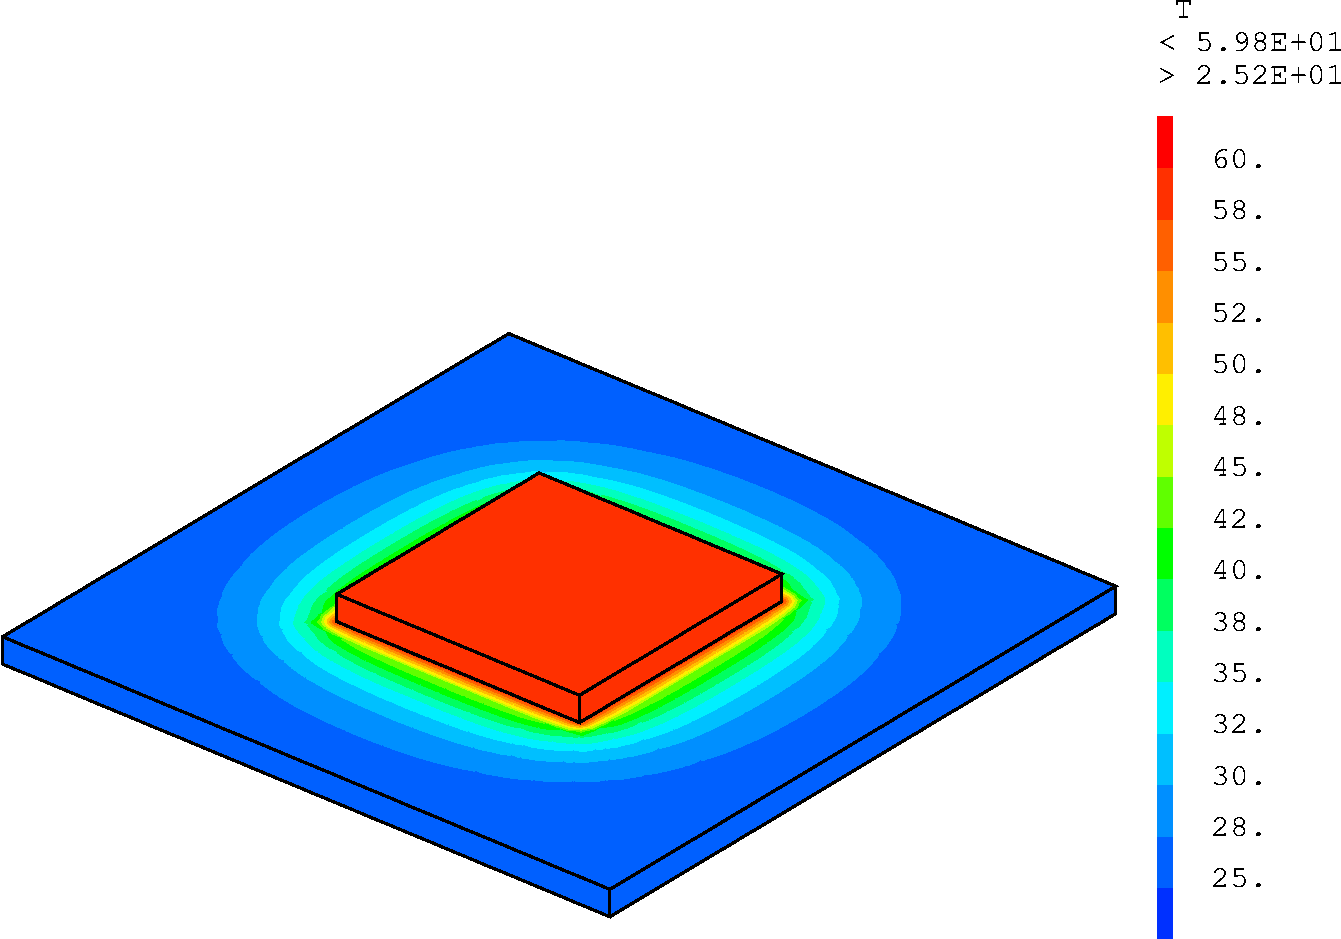
\includegraphics[height=3cm]{images/exo/exo_3_temperature.51} \hspace{0.2cm}
    \fi
    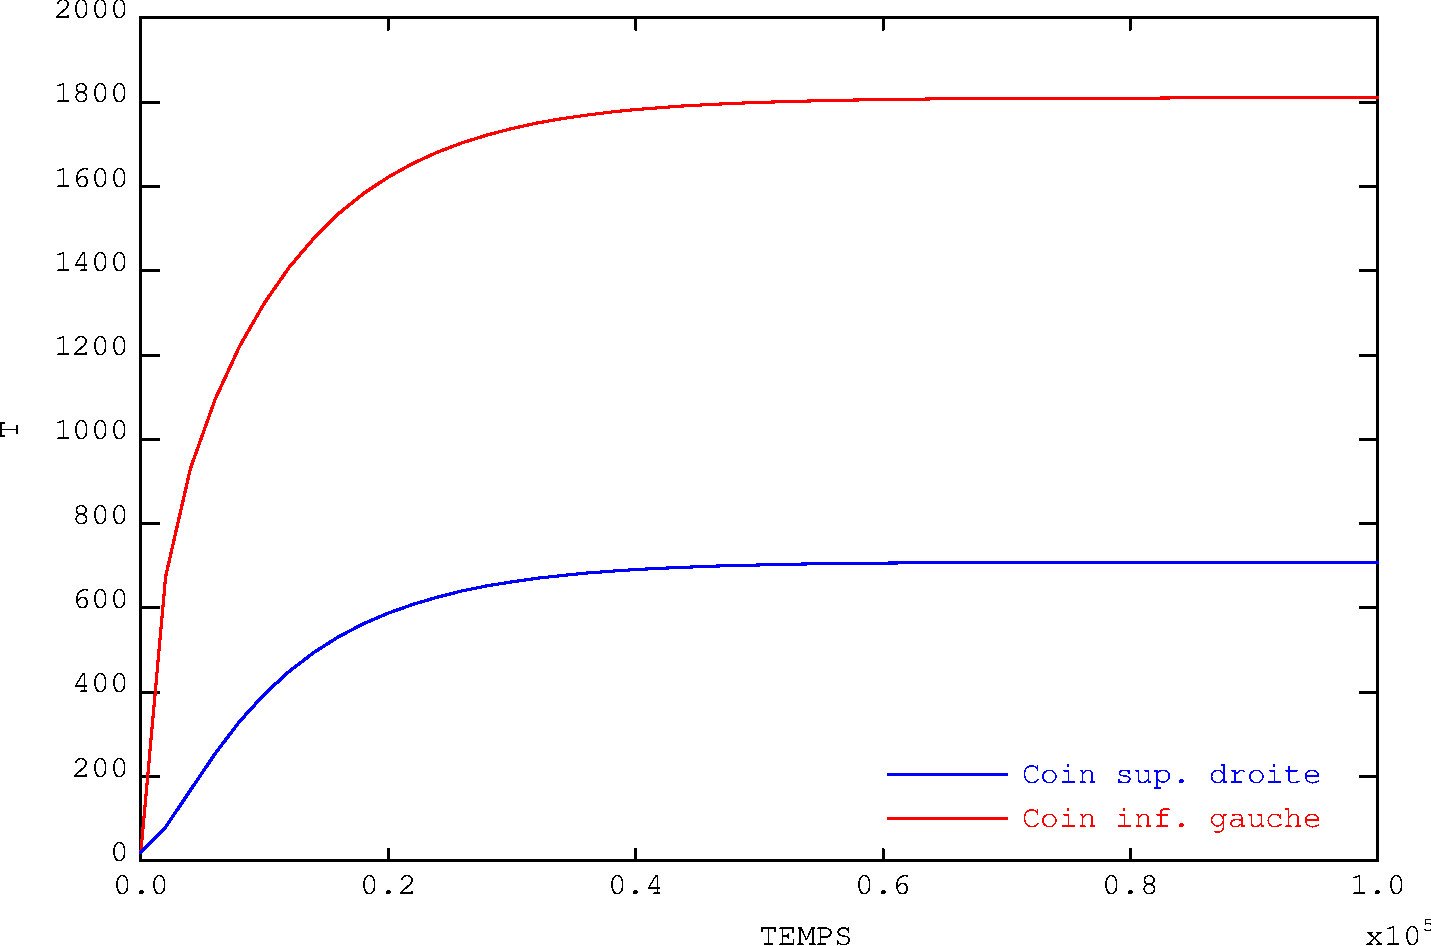
\includegraphics[height=2.6cm]{images/exo/exo_3_evol}
    \small
    \item<2-> \fe{\green{Objectif : rendre le problème \g{variable} !}}
                 {\green{Purpose: make the problem \g{variable}}}\\
    \begin{enumerate}
      \scriptsize
      \item<2-> \fe{\green{Convection fonction du temps}}
                   {\green{Time-dependent convection}}\\
        \begin{textblock*}{6cm}(7.5cm,-0.8cm)
          \tiny
          \begin{tikzpicture}
            \draw[<->,Green] (0,1.8) node (yaxis) [above] {$h$ [W/m$^2$/K]}
                          |- (3,0) node (xaxis) [right] {$t$ [s]};
            \draw[-,red] (0,0.2) node (hmin) [left] {\green{10}} -- (2.5,1.6);
            \draw[dashed] (0,1.6) node (hmax) [left] {\green{200}} -- (2.6,1.6) ;
            \draw[Green] (0,0) node[anchor=north] {0};
            \draw[dashed] (2.5,0) node (tmax) [below] {\green{10$^5$}} -- (2.5,1.75) ;
          \end{tikzpicture}
        \end{textblock*}
      \item<3-> \fe{\green{Conductivité fonction de la température}}
                   {\green{Temperature-dependent conductivity}}\\
                \green{$\lambda (T)=0.3T+200$}
      \item<4-> \fe{\green{Source fonction de la température}}
                   {\green{Temperature-dependent heat source}}\\
                \green{$q(T)=4.10^6~\tx{exp}^{-\left(\frac{T-1000}{700}\right)^2}$}
      \begin{center}
        \fe{\avous{~À vous de jouer !}}{\avous{~It's up to you!}}
      \end{center}
    \end{enumerate}
  \end{itemize}
\end{frame}
}

{\setbeamerfont{framesubtitle}{size=\tiny}
\begin{frame}{\fe{Exercice 3 : dépendance à la température}
                 {Exercise 3: temperature-dependence}}
             {\url{https://www-cast3m.cea.fr/index.php?page=exemples&exemple=formation_pasapas_3_initial}}
  \begin{itemize}
    \item \fe{Quelques objets utiles}{Some useful objects}\\
    \footnotesize
    \kw{sou~~} \fe{maillage de la source de chaleur}{heat source mesh}\\
    \kw{mosou} \fe{modèle thermique réduit sur le maillage de la source}{reduced thermal model on the heat source mesh}\\
    \normalsize
    \item \fe{Quelques opérateurs utiles}{Some useful operators}\\
    \footnotesize
    \kwr{REDU} \fe{réduction des températures sur \kw{sou}}{reduce temperatures on \kw{sou}}\\
    \kwr{SOUR} \fe{imposer une source volumique de chaleur}{impose a volume heat source}\\
    \normalsize
    \item \fe{Quelques indices utiles de la table}{Some useful table indices}\\
    \footnotesize
    \kwg{WTABLE}\kw{.}\kwg{THER\_COURANT} \fe{températures courantes (itérations de \kwo{TRANSNON})}
                                             {current temperatures (\kwo{TRANSNON} iterations)}\\
    \kwg{WTABLE}\kw{.}\kwg{CHARGEMENT} \fe{chargement courant}{current load}
    \normalsize
  \end{itemize}
\end{frame}
}

\begin{frame}{\fe{Exercice 3 : dépendance à la température}
                 {Exercise 3: temperature-dependence}}
             {\fe{Solution avec PERSO2}{Solution with PERSO2}}
  \footnotesize
  \begin{itemize}
    \small
    \item \fe{Utiliser des objets EVOLUTIOn pour $\lambda(T)$ et $h(t)$}{Use EVOLUTIOn objects for $\lambda(T)$ and $h(t)$}
    \item \fe{Utiliser la procédure \kwv{PERSO2}}{Use procedure \kwv{PERSO2}}
    \item \fe{Re-calculer la source selon la température}{Update the source as function of temperature}
    \item \fe{Écraser \kwg{WTABLE}\kw{.}\kwg{CHARGEMENT}}{Overwrite \kwg{WTABLE}\kw{.}\kwg{CHARGEMENT}}
  \end{itemize}
  \vspace{4.5cm}
  \scriptsize
  \begin{textblock*}{10cm}(0.3cm,-4cm)
    \fe{\emph{Programme principal}}{\emph{Main program}}
    \lstinputlisting[basicstyle=\ttfamily\tiny, language=gibiane, firstline=49, lastline=52]{dgibi/formation_pasapas_3_solution.dgibi}
    \lstinputlisting[basicstyle=\ttfamily\tiny, language=gibiane, firstline=56, lastline=59]{dgibi/formation_pasapas_3_solution.dgibi}
    \lstinputlisting[basicstyle=\ttfamily\tiny, language=gibiane, firstline=106, lastline=109]{dgibi/formation_pasapas_3_solution.dgibi}
  \end{textblock*}
  \begin{textblock*}{10cm}(6.cm,-4cm)
    \fe{\emph{\violet{Procédure PERSO2}}}{\emph{\violet{PERSO2 procedure}}}
    \lstinputlisting[basicstyle=\ttfamily\tiny, language=gibiane, firstline=67, lastline=81]{dgibi/formation_pasapas_3_solution.dgibi}
  \end{textblock*}
\end{frame}

\begin{frame}{\fe{Exercice 3 : dépendance à la température}
                 {Exercise 3: temperature-dependence}}
             {\fe{Solution avec CHARTHER}{Solution with CHARTHER}}
  \footnotesize
  \begin{itemize}
    \small
    \item \fe{Idem mais avec la procédure \kwv{CHARTHER}}{Idem but with the \kwv{CHARTHER} procedure}
    \item \fe{Pas besoin de CHARGEMEnt initial}{No need for initial load (CHARGEMEnt object)}
  \end{itemize}
  \vspace{4.5cm}
  \scriptsize
  \begin{textblock*}{10cm}(0.3cm,-4cm)
    \fe{\emph{Programme principal}}{\emph{Main program}}
    \lstinputlisting[basicstyle=\ttfamily\tiny, language=gibiane, firstline=49, lastline=52]{dgibi/formation_pasapas_3_solution.dgibi}
    \lstinputlisting[basicstyle=\ttfamily\tiny, language=gibiane, firstline=56, lastline=59]{dgibi/formation_pasapas_3_solution.dgibi}
    \lstinputlisting[basicstyle=\ttfamily\tiny, language=gibiane, firstline=147, lastline=152]{dgibi/formation_pasapas_3_solution.dgibi}
  \end{textblock*}
  \begin{textblock*}{10cm}(6.cm,-4cm)
    \fe{\emph{\violet{Procédure CHARTHER}}}{\emph{\violet{CHARTHER procedure}}}
    \lstinputlisting[basicstyle=\ttfamily\tiny, language=gibiane, firstline=84, lastline=98]{dgibi/formation_pasapas_3_solution.dgibi}
  \end{textblock*}
\end{frame}

\begin{frame}{\fe{Exercice 3 : dépendance à la température}
                 {Exercise 3: temperature-dependence}}
  \begin{itemize}
    \item \fe{Résultats}{Results}\\
    \vspace{5cm}
    \begin{textblock*}{5cm}(0.5cm,-5cm)
      \if \animation 1
        \animategraphics[controls,loop,poster=last,width=5cm]{7}{images/exo/exo_3_solu_temperature.}{01}{51}
      \else
        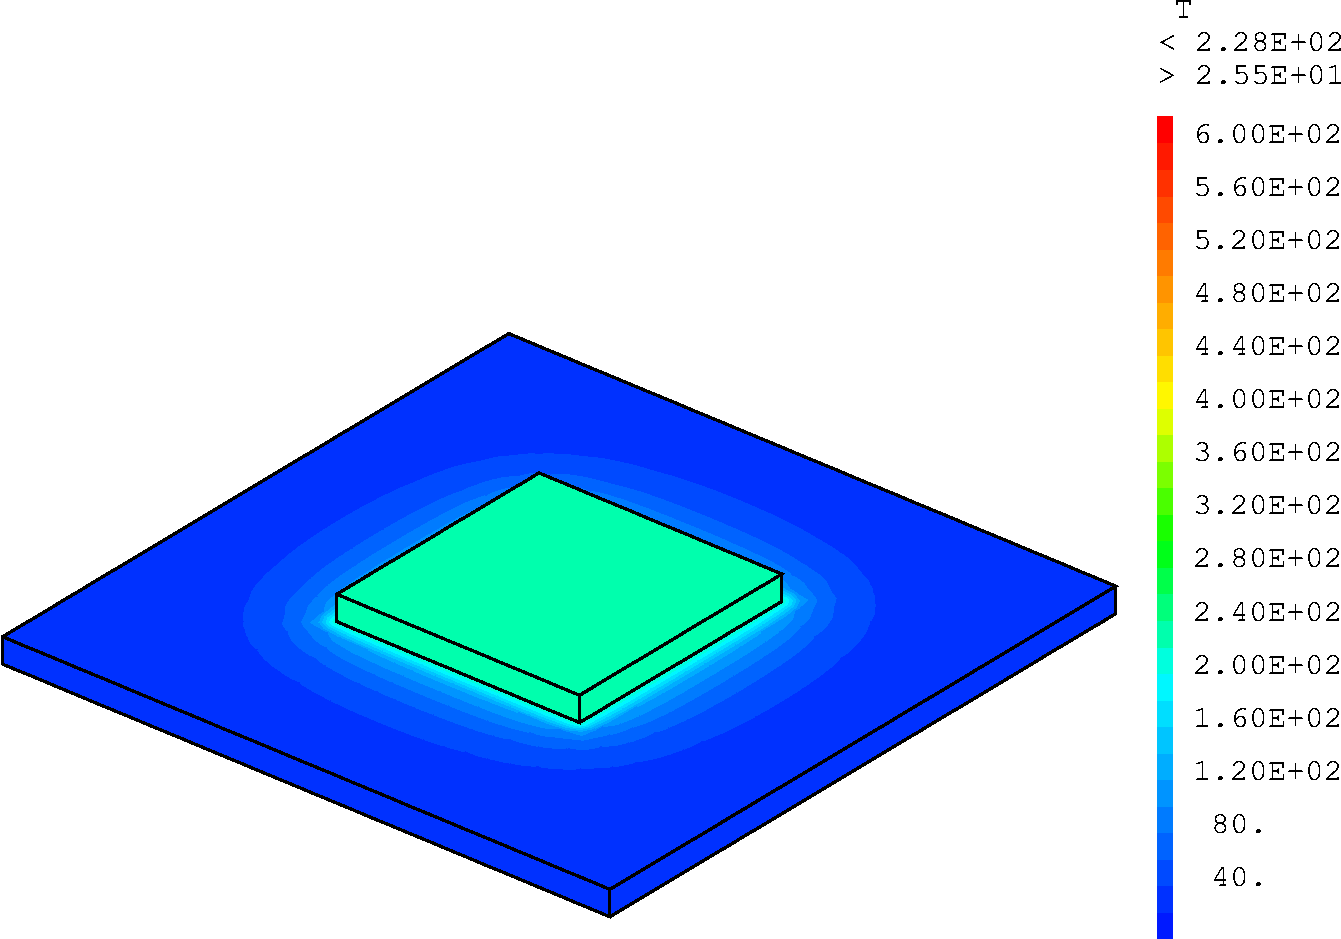
\includegraphics[width=5cm]{images/exo/exo_3_solu_temperature.51}
      \fi
      \end{textblock*}
    \footnotesize
    \begin{textblock*}{5cm}(6.3cm,-6cm)
      \fe{Avec \kwv{PERSO2}}{With \kwv{PERSO2}}
      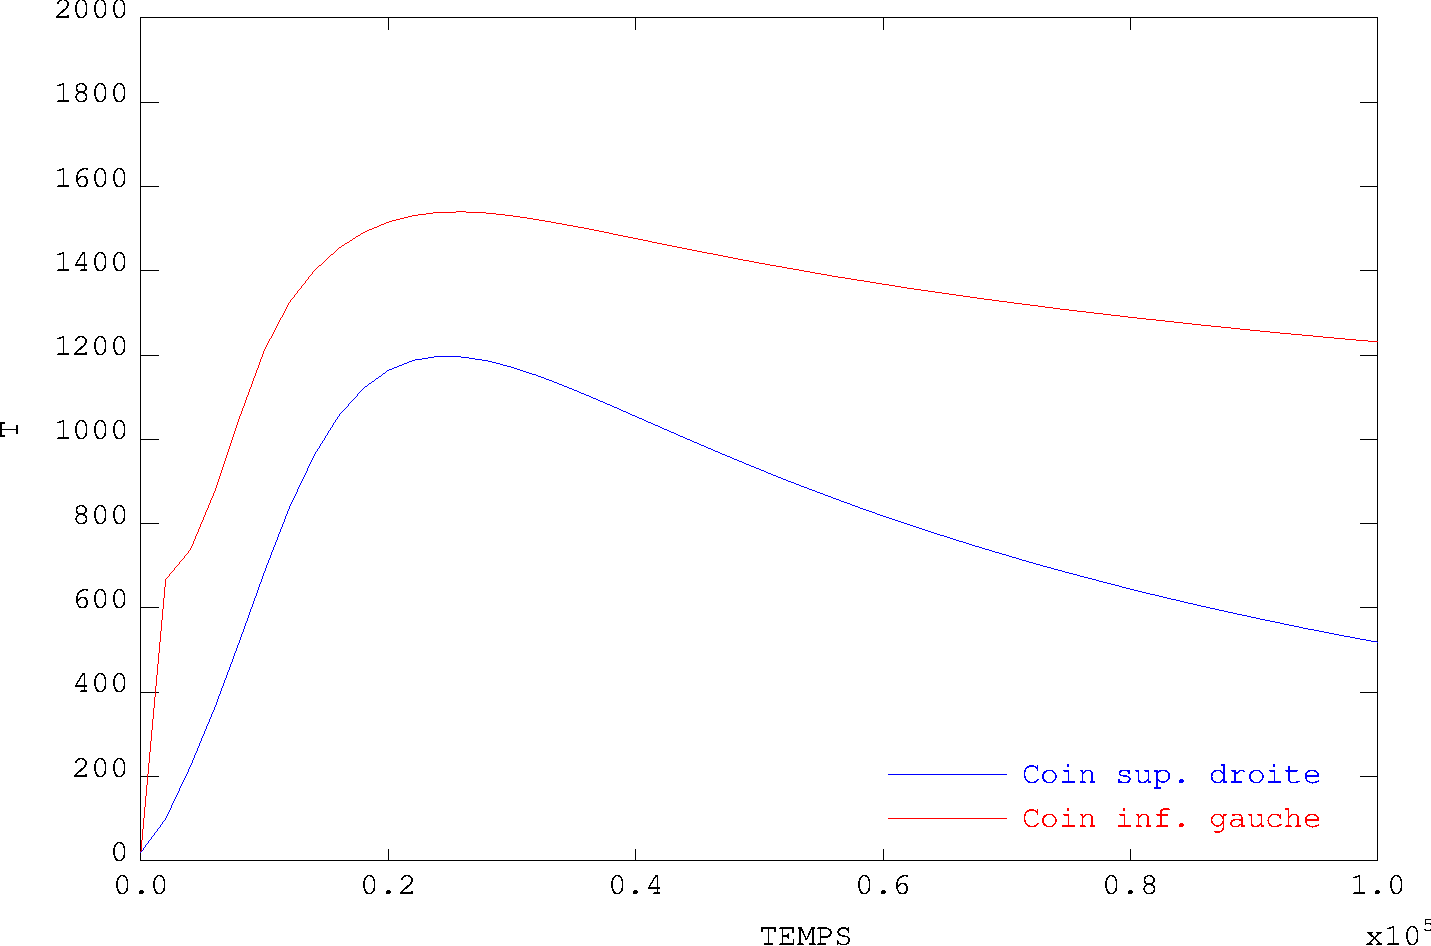
\includegraphics[width=5cm]{images/exo/exo_3_solu_evol}
    \end{textblock*}
    \begin{textblock*}{5cm}(6.3cm,-2cm)
      \fe{Avec \kwv{CHARTHER}}{With \kwv{CHARTHER}}
      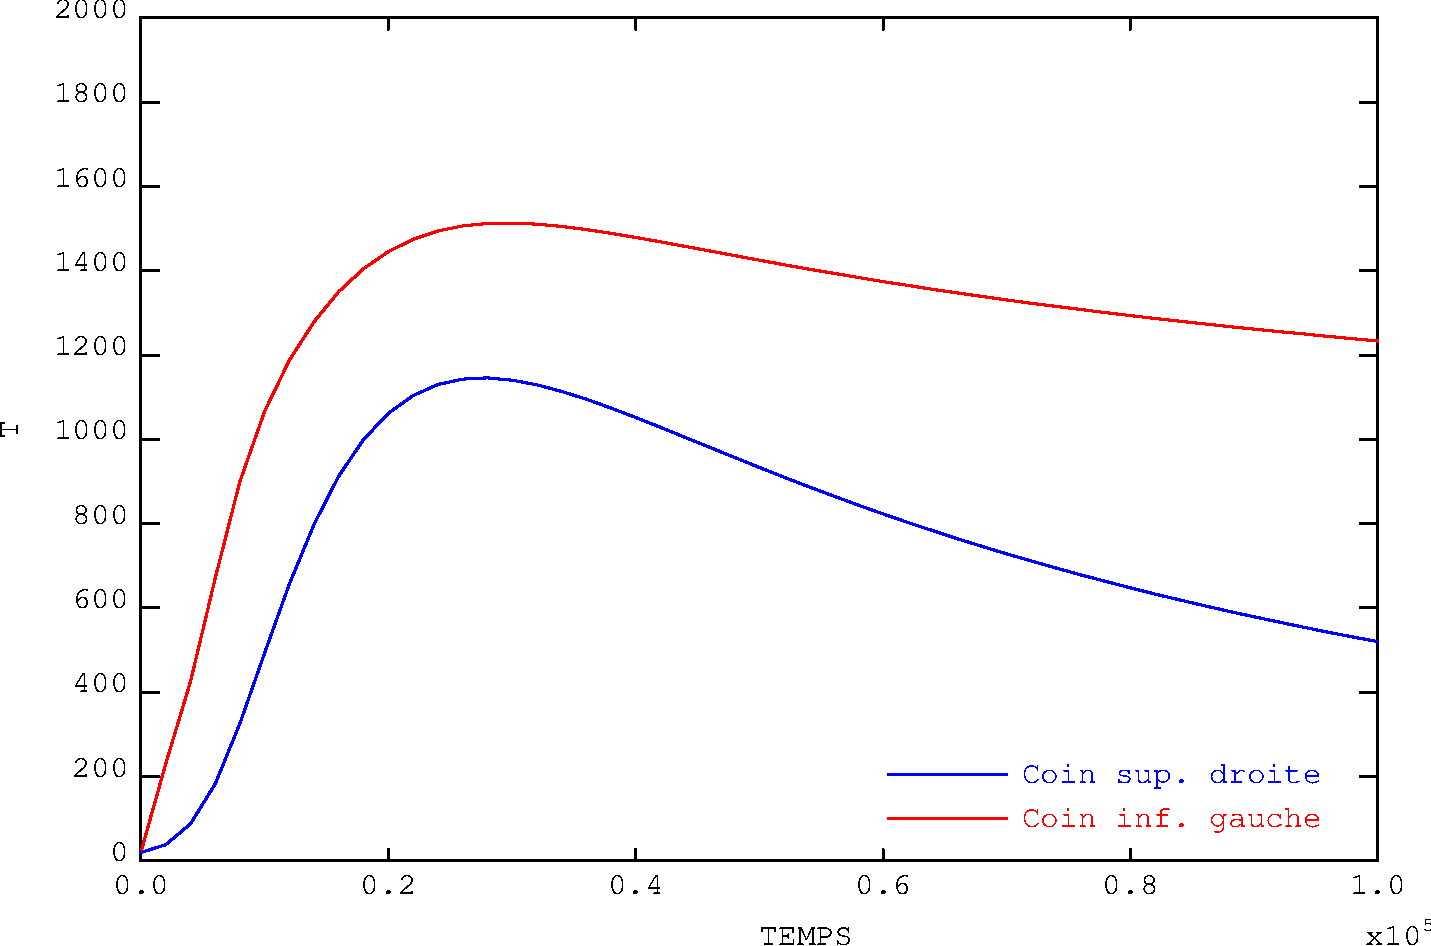
\includegraphics[width=5cm]{images/exo/exo_3_solu_bis_evol}
    \end{textblock*}
  \end{itemize}
\end{frame}

% {\setbeamerfont{framesubtitle}{size=\tiny}
\begin{frame}{\fe{Exercice 4 : contact thermo mécanique}
                 {Exercise 4: thermo mechanical contact}}
             {\url{https://www-cast3m.cea.fr/index.php?page=exemples&exemple=formation_pasapas_4_initial}}
  \small
  \begin{itemize}
    \item \fe{Dilatation thermique de 2 barreaux et mise en contact}
             {Thermal expansion of 2 bars and coming into contact}
  \end{itemize}
  \begin{center}
    \begin{tikzpicture}
      \scriptsize
      \def\lbar{4}  \def\hbar{1}   \def\gap{1.2}
      \draw [-] (0,0)          -- (-0.1,-0.1)           -- (-0.1,0.1)            --cycle;
      \draw [-] (0,0.33*\hbar) -- (-0.1,0.33*\hbar-0.1) -- (-0.1,0.33*\hbar+0.1) --cycle;
      \draw [-] (0,0.66*\hbar) -- (-0.1,0.66*\hbar-0.1) -- (-0.1,0.66*\hbar+0.1) --cycle;
      \draw [-] (0,\hbar)      -- (-0.1,\hbar-0.1)      -- (-0.1,\hbar+0.1)      --cycle;
      \draw[fill=red!30] (0,0) rectangle (\lbar,\hbar);
      \filldraw (0,0)     circle(0.4mm) node[anchor=north west] {\kw{p1}};
      \filldraw (\lbar,0) circle(0.4mm) node[anchor=north east] {\kw{p2}};
      \draw (\lbar,0.5*\hbar) node[anchor=west] {\kw{l2}};
      \draw (0.5*\lbar,0.5*\hbar) node {\fe{Barreau 1}{Bar 1} \red{$T_{\tx{ini}}=20$°C}};
      \draw [->,thick,red] (0.4,\hbar+0.2) node[anchor=west] {$T_{\tx{imp}}=500$°C} -- (0,0.5*\hbar);
      \draw [-] (2*\lbar+\gap,0)          -- (2*\lbar+\gap+0.1,-0.1)           -- (2*\lbar+\gap+0.1,0.1)            --cycle;
      \draw [-] (2*\lbar+\gap,0.33*\hbar) -- (2*\lbar+\gap+0.1,0.33*\hbar-0.1) -- (2*\lbar+\gap+0.1,0.33*\hbar+0.1) --cycle;
      \draw [-] (2*\lbar+\gap,0.66*\hbar) -- (2*\lbar+\gap+0.1,0.66*\hbar-0.1) -- (2*\lbar+\gap+0.1,0.66*\hbar+0.1) --cycle;
      \draw [-] (2*\lbar+\gap,\hbar)      -- (2*\lbar+\gap+0.1,\hbar-0.1)      -- (2*\lbar+\gap+0.1,\hbar+0.1)      --cycle;
      \draw[fill=blue!30] (\lbar+\gap,0) rectangle (2*\lbar+\gap,\hbar);
      \filldraw (\lbar+\gap,0)   circle(0.4mm) node[anchor=north west] {\kw{p3}};
      \filldraw (2*\lbar+\gap,0) circle(0.4mm) node[anchor=north east] {\kw{p4}};
      \draw (\lbar+\gap,0.5*\hbar) node[anchor=east] {\kw{l3}};
      \draw (1.5*\lbar+\gap,0.5*\hbar) node {\fe{Barreau 2}{Bar 2} \blue{$T_{\tx{ini}}=20$°C}};
      \draw [->,thick,blue] (2*\lbar+\gap-0.4,\hbar+0.2) node[anchor=east] {$T_{\tx{imp}}=20$°C} -- (2*\lbar+\gap,0.5*\hbar);
    \end{tikzpicture}\\
    \vspace{0.5cm}
    \animategraphics[controls,loop,poster=first,width=10cm]{12}{images/exo/exo_4_temperature.}{001}{101}
  \end{center}
  \begin{itemize}
    \item<2-> \fe{\green{Objectif : ajouter le \g{contact thermique} entre \kw{l2} et \kw{l3},\\
                        \qquad \qquad ~ c'est à dire le transfert de chaleur lors du contact.}}
                {\green{Purpose: add \g{thermal contact} between \kw{l2} and \kw{l3},\\
                        \qquad \qquad this means the heat transfer when contact takes place.}}\\
    \begin{center}
      \fe{\avous{~À vous de jouer !}}{\avous{~It's up to you!}}
    \end{center}
  \end{itemize}
\end{frame}
}

{\setbeamerfont{framesubtitle}{size=\tiny}
\begin{frame}{\fe{Exercice 4 : contact thermo mécanique}
                 {Exercise 4: thermo mechanical contact}}
             {\url{https://www-cast3m.cea.fr/index.php?page=exemples&exemple=formation_pasapas_4_initial}}
  \begin{itemize}
    \item \fe{Quelques objets utiles}{Some useful objects}\\
    \footnotesize
    \kw{p2 p3} \fe{points à gauche et à droite du jeu}{points on the left/right of the gap}\\
    \kw{l2 l3} \fe{lignes à gauche et droite du jeu}{lines on the left/right of the gap}\\
    \normalsize
    \item \fe{Quelques opérateurs utiles}{Some useful operators}\\
    \footnotesize
    \kwr{COOR} \fe{obtenir les coordonnées de points}{get points coordinates}\\
    \kwr{RELA} \fe{imposer une relation linéaire entre degrés de liberté}{impose a linear relation between degrees of freedom}\\
    \normalsize
    \item \fe{Quelques indices utiles de la table}{Some useful table indices}\\
    \footnotesize
    \kwg{WTABLE}\kw{.}\kwg{BLOCAGES\_THERMIQUES} \fe{CL thermiques courrantes}{current thermal BC}\\
    \normalsize
  \end{itemize}
\end{frame}
}

\begin{frame}{\fe{Exercice 4 : contact thermo mécanique}
                 {Exercise 4: thermo mechanical contact}}
             {\fe{Solution avec REEV\_MEC}{Solution with REEV\_MEC}}
  \footnotesize
  \begin{itemize}
    \item \fe{Créer une \kwr{RELA}tion entre les températures de \kw{l2} et \kw{l3}}
             {Create a \kwr{RELA}tion between temperatures at \kw{l2} and \kw{l3}}
    \item \fe{Utiliser la \red{boucle de convergence thermo mécanique}}{Use the \red{thermo mechanical convergence loop}}
    \item \fe{Utiliser la procédure \kwv{REEV\_MEC}}{Use procedure \kwv{REEV\_MEC}}
    \item \fe{Calculer le jeu à l'itération courante et modifier (ou non) l'indice \kwg{WTABLE}\kw{.}\kwg{BLOCAGES\_THERMIQUES}}
             {Calculate the gap at current iteration and modifiy \kwg{WTABLE}\kw{.}\kwg{BLOCAGES\_THERMIQUES} or not}
  \end{itemize}
  \vspace{4.5cm}
  \scriptsize
  \begin{textblock*}{10cm}(0.3cm,-4.5cm)
    \fe{\emph{Programme principal}}{\emph{Main program}}
    \lstinputlisting[basicstyle=\ttfamily\tiny, language=gibiane, firstline=103, lastline=110]{dgibi/formation_pasapas_4_solution.dgibi}
  \end{textblock*}
  \begin{textblock*}{10cm}(5.6cm,-4.5cm)
    \fe{\emph{\violet{Procédure REEV\_MEC}}}{\emph{\violet{REEV\_MEC procedure}}}
    \lstinputlisting[basicstyle=\ttfamily\tiny, language=gibiane, firstline=78, lastline=93]{dgibi/formation_pasapas_4_solution.dgibi}
  \end{textblock*}
\end{frame}

\begin{frame}{\fe{Exercice 4 : contact thermo mécanique}
                 {Exercise 4: thermo mechanical contact}}
             {\fe{Solution avec REEV\_MEC}{Solution with REEV\_MEC}}
  \begin{itemize}
    \item \fe{Résultats}{Results}
  \end{itemize}
  \begin{center}
    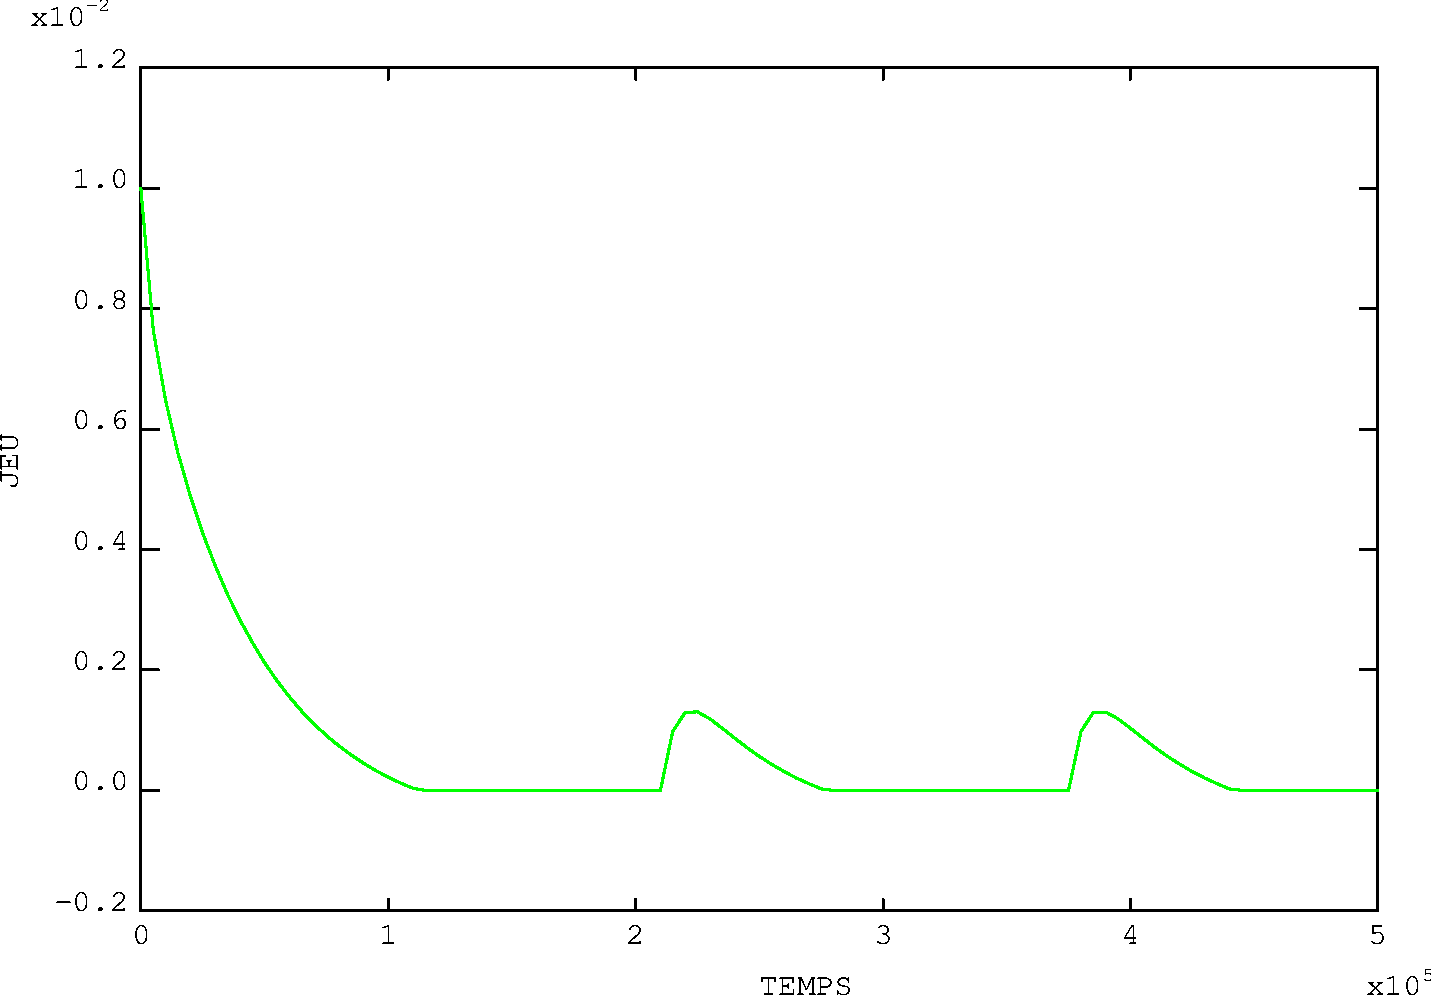
\includegraphics[width=5.5cm]{images/exo/exo_4_solu_evol_jeu}
    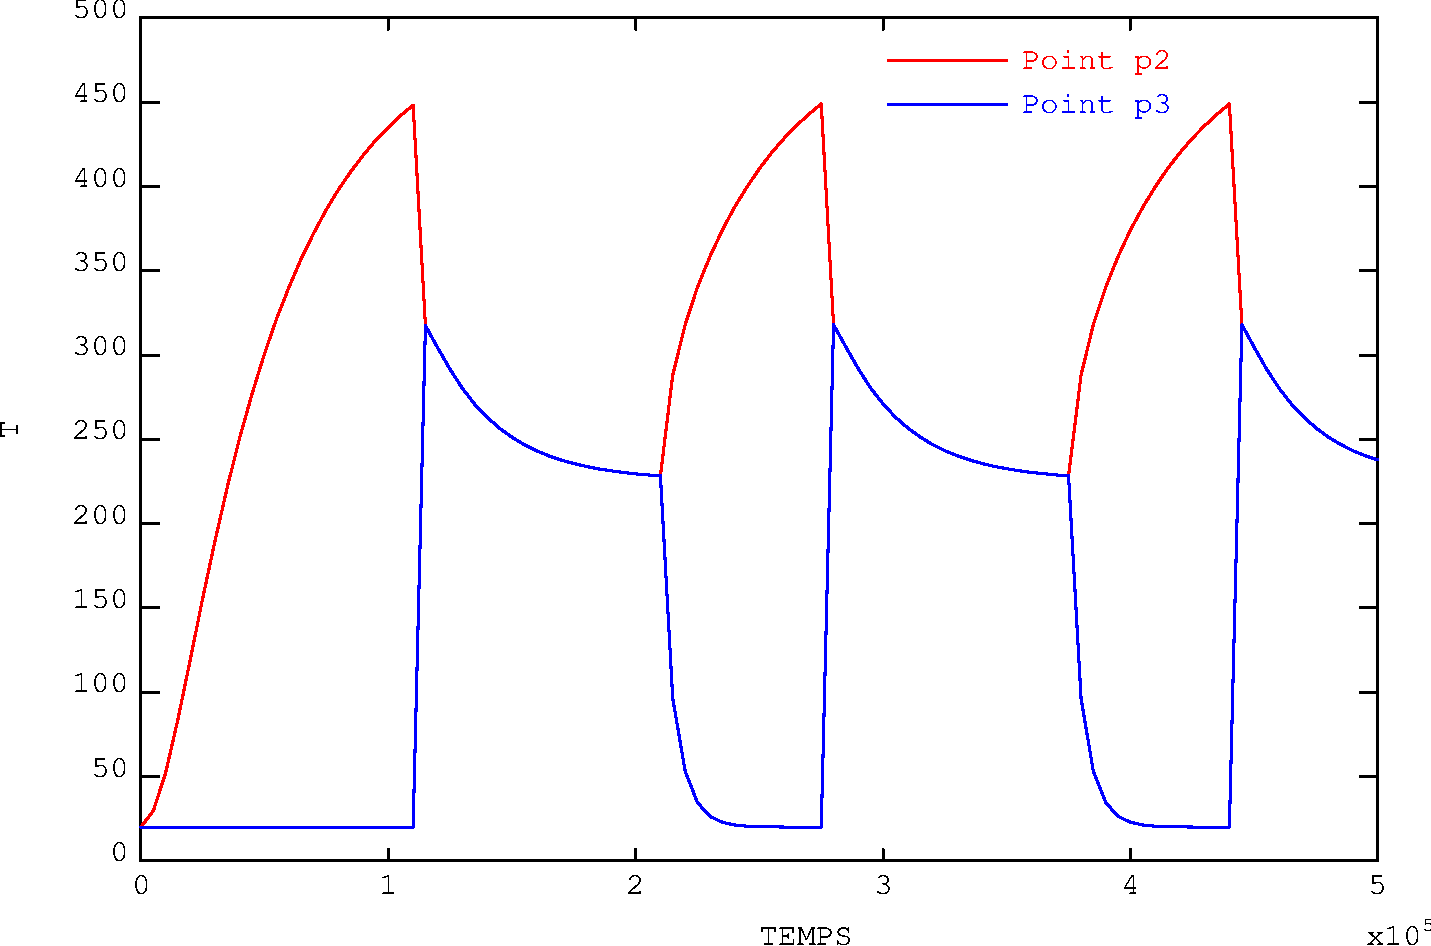
\includegraphics[width=5.5cm]{images/exo/exo_4_solu_evol_t}\\
    \vspace{0.5cm}
    \animategraphics[controls,loop,poster=first,width=10.5cm]{12}{images/exo/exo_4_solu_temperature.}{001}{101}
  \end{center}
\end{frame}

\begin{frame}{\fe{Exercice 4 : contact thermo mécanique}
                 {Exercise 4: thermo mechanical contact}}
             {\fe{Solution (bis) avec REEV\_MEC}{Solution (bis) with REEV\_MEC}}
  \footnotesize
  \begin{itemize}
    \item \fe{Transfert par convection à l'interface avec des éléments de \kwr{RACC}ord\\
              \scriptsize coefficient d'échange dépendant de la pression \footnotesize}
             {Convective heat transfert at the interface with transition elements\\
             \scriptsize coefficient depending on pressure \footnotesize}
    \item \fe{Utiliser un objet CHARGEMEnt pour décrire la valeur de pression\\
              \scriptsize et mettre à jour ce chargement avec \kwv{REEV\_MEC} \footnotesize}
             {Use a CHARGEME object to describe pressure value\\
             \scriptsize and update this load with \kwv{REEV\_MEC} \footnotesize}
  \end{itemize}
  \vspace{4.5cm}
  \scriptsize
  \only<1>{
    \begin{textblock*}{10cm}(2cm,-4.3cm)
      \fe{\emph{Programme principal}}{\emph{Main program}}
      \lstinputlisting[basicstyle=\ttfamily\tiny, language=gibiane, firstline=82, lastline=85]{dgibi/formation_pasapas_4_solution_bis.dgibi}
      \lstinputlisting[basicstyle=\ttfamily\tiny, language=gibiane, firstline=88, lastline=89]{dgibi/formation_pasapas_4_solution_bis.dgibi}
      \lstinputlisting[basicstyle=\ttfamily\tiny, language=gibiane, firstline=110, lastline=111]{dgibi/formation_pasapas_4_solution_bis.dgibi}
      \lstinputlisting[basicstyle=\ttfamily\tiny, language=gibiane, firstline=114, lastline=114]{dgibi/formation_pasapas_4_solution_bis.dgibi}
      \lstinputlisting[basicstyle=\ttfamily\tiny, language=gibiane, firstline=116, lastline=121]{dgibi/formation_pasapas_4_solution_bis.dgibi}
    \end{textblock*}
  }
  \only<2>{
    \begin{textblock*}{10cm}(3cm,-4.3cm)
      \fe{\emph{\violet{Procédure REEV\_MEC}}}{\emph{\violet{REEV\_MEC procedure}}}
      \lstinputlisting[basicstyle=\ttfamily\tiny, language=gibiane, firstline=92, lastline=106]{dgibi/formation_pasapas_4_solution_bis.dgibi}
    \end{textblock*}
  }
\end{frame}

\begin{frame}{\fe{Exercice 4 : contact thermo mécanique}
                 {Exercise 4: thermo mechanical contact}}
             {\fe{Solution (bis) avec REEV\_MEC}{Solution (bis) with REEV\_MEC}}
  \begin{itemize}
    \item \fe{Résultats}{Results}
  \end{itemize}
  \begin{center}
    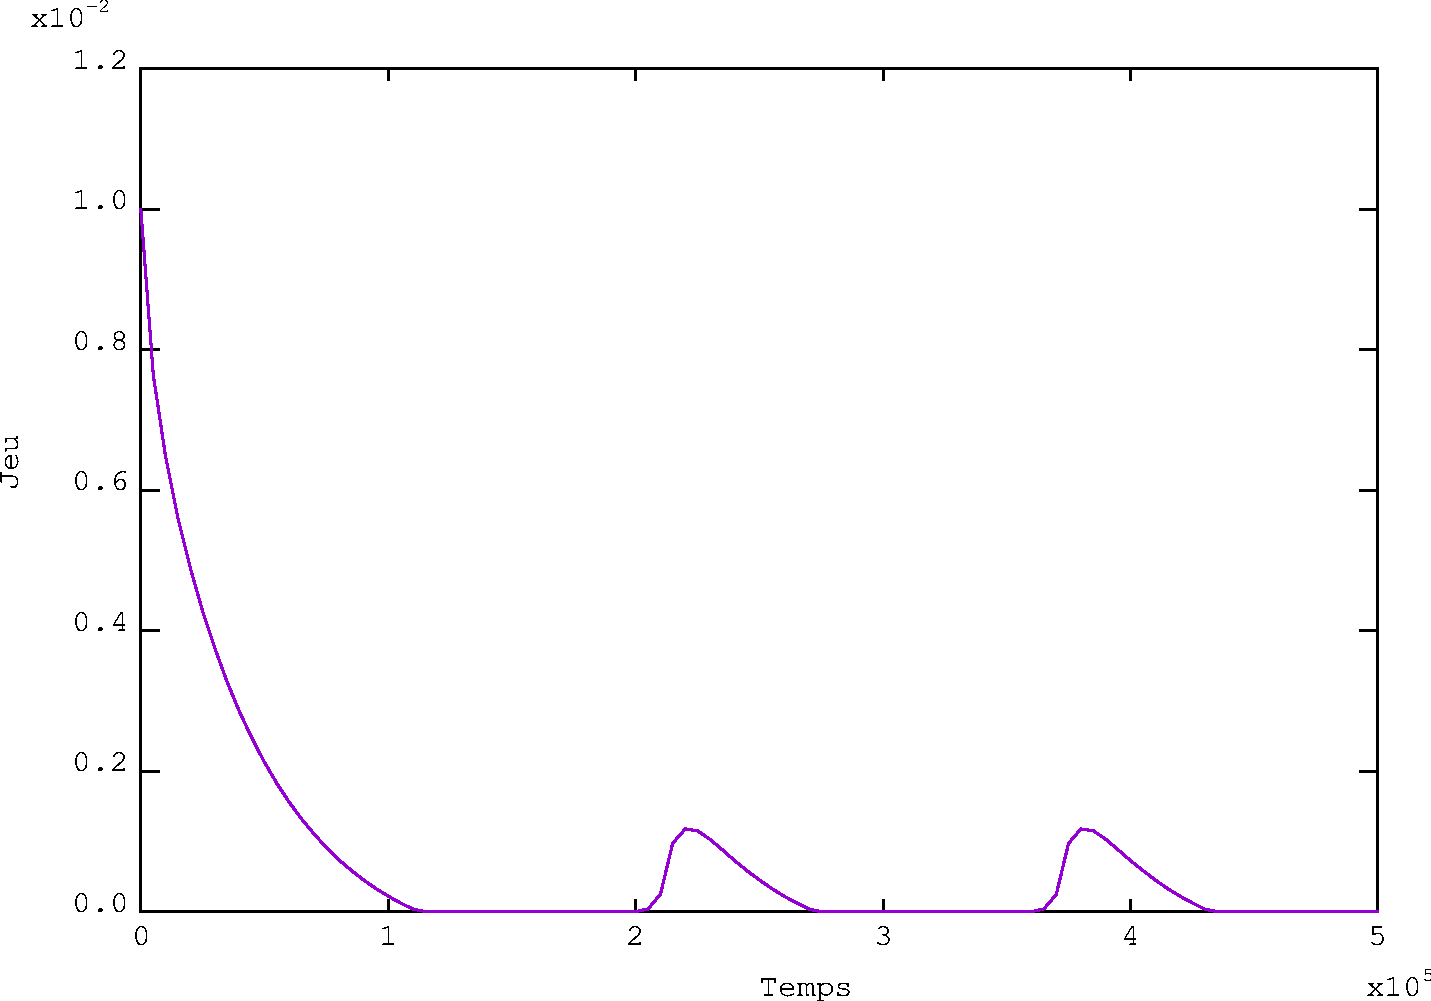
\includegraphics[width=5.5cm]{images/exo/exo_4_solu_bis_evol_jeu}
    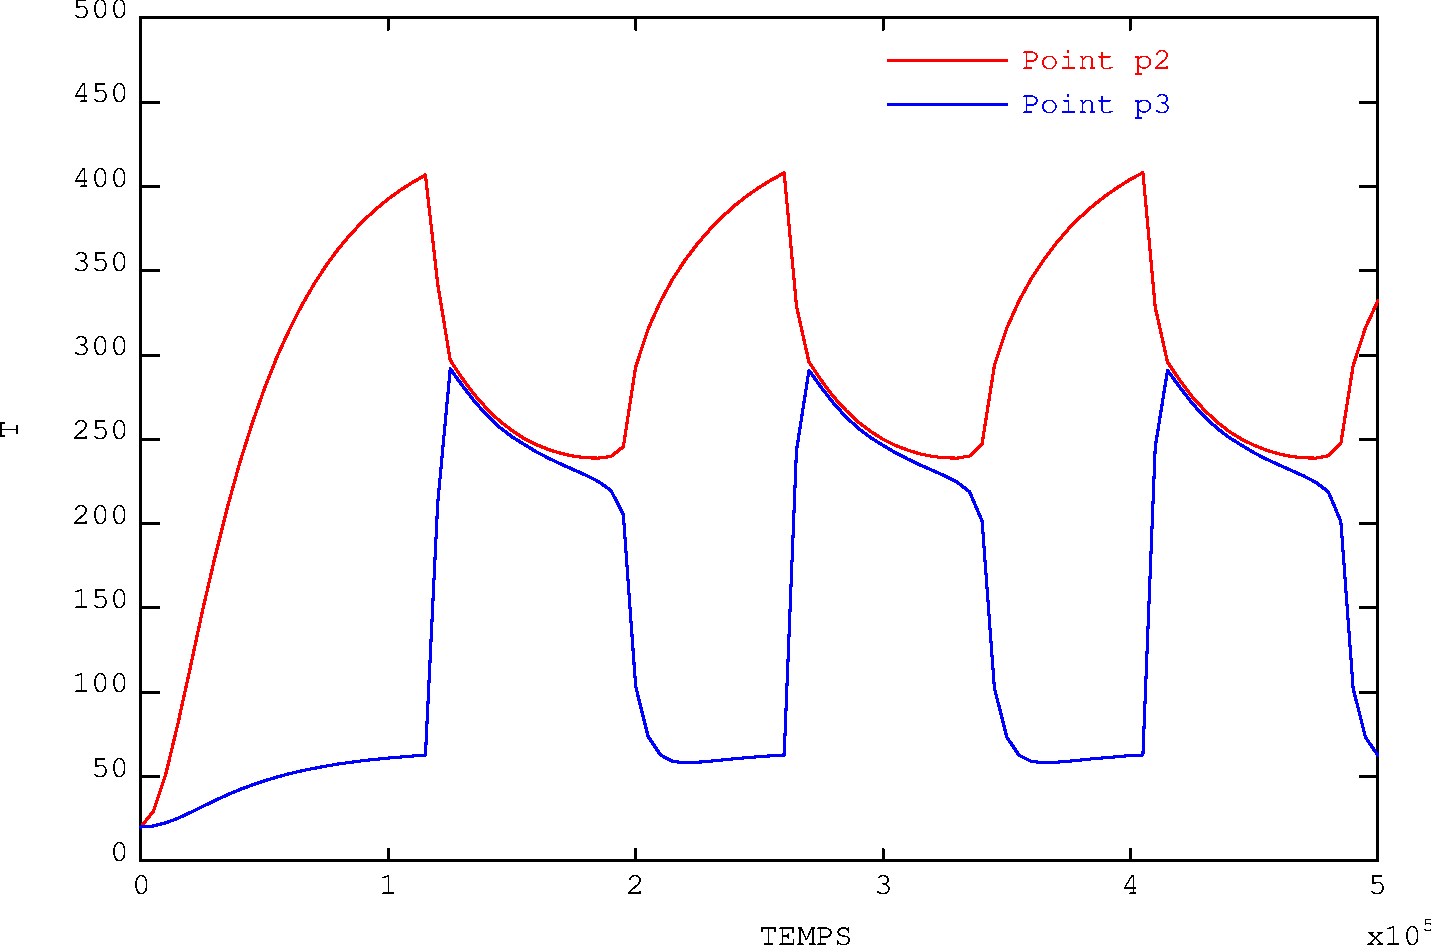
\includegraphics[width=5.5cm]{images/exo/exo_4_solu_bis_evol_t}\\
    \vspace{0.5cm}
    \animategraphics[controls,loop,poster=first,width=10.5cm]{12}{images/exo/exo_4_solu_bis_temperature.}{001}{101}
  \end{center}
\end{frame}

% % Remplacer les apostrophes ’ par des quotes '
% Exo 1 : mettre les grands deplacements initialement


\begin{frame}{\fe{Exercice 3 : dépendance à la température}
                 {Exercise 3: temperature-dependence}}
             {\fe{Solution avec PERSO2}{Solution with PERSO2}}
  \footnotesize
  \begin{itemize}
    \small
    \item \fe{Utiliser la procédure \kwv{PERSO2}}{Use procedure \kwv{PERSO2}}
  \end{itemize}
  \vspace{4.5cm}
  \scriptsize
  \begin{textblock*}{10cm}(0.3cm,-3.2cm)
    \fe{\emph{Programme principal}}{\emph{Main program}}
  \end{textblock*}
  \begin{textblock*}{10cm}(6.2cm,-4cm)
    \fe{\emph{\violet{Procédure PERSO2}}}{\emph{\violet{PERSO2 procedure}}}
  \end{textblock*}
\end{frame}

\begin{frame}{\fe{Exercice 3 : dépendance à la température}
                 {Exercise 3: temperature-dependence}}
  \footnotesize
  \begin{itemize}
    \item \fe{Résultats}{Results}\\
    \hspace{1cm}
  \end{itemize}
\end{frame}



\end{document}
